% This is a modified version of the tufte-latex book example in which the title page and the contents page resemble Tufte's VDQI book, using Kevin Godby's code from this thread at https://groups.google.com/forum/#!topic/tufte-latex/ujdzrktC1BQ.
%
%%%%%%%%%%%%%%%%%%%%%%%%%%%%%%%%%%%%%%%%%%%%%%%%%%%%%%%%%%%%%%%%%%%%%%
% How to use Overleaf: 
%
% You edit the source code here on the left, and the preview on the
% right shows you the result within a few seconds.
%
% Bookmark this page and share the URL with your co-authors. They can
% edit at the same time!
%
% You can upload figures, bibliographies, custom classes and
% styles using the files menu.
%
% If you're new to LaTeX, the wikibook is a great place to start:
% http://en.wikibooks.org/wiki/LaTeX
%
%%%%%%%%%%%%%%%%%%%%%%%%%%%%%%%%%%%%%%%%%%%%%%%%%%%%%%%%%%%%%%%%%%%%%%
%% Unfortunately for the contents to contain
%% the "Parts" lines successfully, hyperref
%% needs to be disabled.

% 1q1

\documentclass[a4paper,nofonts,notoc,oneside,openany,nobib]{tufte-book}
\usepackage{geometry}
\usepackage{bm}
% \usepackage{float}
\geometry{
  % showframe,
  % paperwidth=6in,
  % paperheight=9in,
  left=0.5in,
  right=0.5in,
  top=.2in,
  bottom=.5in,
  marginparsep=0.2in,
  marginparwidth=2in,
  includemp,
  includehead,
  % The text width and height are calculated automatically.
}


\newcommand{\formatpart}[1]{%
\begin{fullwidth}
    \centering%
    \partname~\thepart%
    \newline%
    #1%
\end{fullwidth}
    }


% TITLE FORMATTING

\titleformat% Formatting the part header
  {\part} % command
  [block] % shape
  {\bfseries\huge} % format
  {} % label
  {0pt} % sep
  { \formatpart
}%

\titleformat
  {\section}
  [block]
  {\bfseries\itshape\LARGE\raggedright}
  {\thesection}
  {1em}
  {}


\titleformat
  {\subsection}
  [block]
  {\bfseries\itshape\Large\raggedright}
  {\thesubsection}
  {1em}
  {}





%  GENERAL SETUP
\setcounter{tocdepth}{1}
\setcounter{secnumdepth}{2}
\usepackage{nameref}
\hypersetup{colorlinks}
\usepackage{ragged2e}

% uncomment this line if you prefer colored hyperlinks (e.g., for onscreen viewing)

% This is preamble.tex

% Commented out the following packages as requested

\usepackage{amsmath,amsfonts,amsthm,amssymb,mathtools}

% \usepackage{bookmark}
\usepackage{enumitem}
% \usepackage{hyperref,theoremref}
\usepackage[most,many,breakable]{tcolorbox}
\usepackage{xcolor}
\usepackage{pgfplots}
\pgfplotsset{compat=1.17}
\usepgfplotslibrary{colormaps}
\usetikzlibrary{matrix, calc, positioning, arrows.meta, shapes.geometric, bbox}


\usepackage{algorithm, algpseudocode}

\usepackage{tabularx}

% Redefine \subsubsection with bold and larger text
\renewcommand{\subsubsection}[1]{%
  \vspace{0.5em}
  \textbf{\large #1}\mbox{}\\
  \vspace{0.5em}}

  
\newcommand{\RR}{\mathbb{R}}




% Color definitions
\definecolor{myg}{RGB}{56, 140, 70}
\definecolor{myb}{RGB}{45, 111, 177}
\definecolor{myp}{RGB}{197, 92, 212}
\definecolor{mytheorembg}{HTML}{F2F2F9}
\definecolor{mytheoremfr}{HTML}{00007B}
\definecolor{myexamplebg}{HTML}{F2FBF8}
\definecolor{myexamplefr}{HTML}{88D6D1}
\definecolor{myexampleti}{HTML}{2A7F7F}

% Define the shared counter
\newcounter{definition}[section]
\newcounter{extra}[section]
\newcounter{sidenote}[section]
\newcounter{example}[section]
\newcounter{exam}[section]
\newcounter{reference}[section]
\newcounter{intuition}[section]

% Theorem styles with selective font changes
\tcbuselibrary{theorems,skins,hooks}
\newtcbtheorem[number within=section]{Theorem}{Theorem}
{enhanced, breakable=false, colback=mytheorembg, frame hidden, boxrule=0sp, 
 borderline west={2pt}{0pt}{mytheoremfr}, sharp corners, detach title, 
 before upper={\renewcommand{\familydefault}{\sfdefault}\selectfont\tcbtitle\par\smallskip}, 
 coltitle=mytheoremfr, fonttitle=\bfseries\sffamily, description font=\mdseries, 
 separator sign none, segmentation style={solid, mytheoremfr}}{th}

\newtcbtheorem[number within=section]{corollary}{Corollary}
{enhanced, breakable=false, colback=myp!10, frame hidden, boxrule=0sp, 
 borderline west={2pt}{0pt}{myp!85!black}, sharp corners, detach title, 
 before upper={\renewcommand{\familydefault}{\sfdefault}\selectfont\tcbtitle\par\smallskip}, 
 coltitle=myp!85!black, fonttitle=\bfseries\sffamily, description font=\mdseries, 
 separator sign none, segmentation style={solid, myp!85!black}}{th}

\newtcbtheorem[number within=section]{lemma}{Lemma}
{enhanced, breakable=false, colback=myg!10, frame hidden, boxrule=0sp, 
 borderline west={2pt}{0pt}{myg}, sharp corners, detach title, 
 before upper={\renewcommand{\familydefault}{\sfdefault}\selectfont\tcbtitle\par\smallskip}, 
 coltitle=myg!85!black, fonttitle=\bfseries\sffamily, description font=\mdseries, 
 separator sign none, segmentation style={solid, myg!85!black}}{th}

\newtcbtheorem[number within=section]{claim}{Claim}
{enhanced, breakable=false, colback=myg!10, frame hidden, boxrule=0sp, 
 borderline west={2pt}{0pt}{myg}, sharp corners, detach title, 
 before upper={\renewcommand{\familydefault}{\sfdefault}\selectfont\tcbtitle\par\smallskip}, 
 coltitle=myg!85!black, fonttitle=\bfseries\sffamily, description font=\mdseries, 
 separator sign none, segmentation style={solid, myg!85!black}}{th}

\newtcbtheorem[number within=section]{Example}{Example}
{colback=myexamplebg, breakable=false, colframe=myexamplefr, coltitle=myexampleti, 
 boxrule=1pt, sharp corners, detach title, 
 before upper={\renewcommand{\familydefault}{\sfdefault}\selectfont\tcbtitle\par\smallskip}, 
 fonttitle=\bfseries\sffamily, description font=\mdseries, 
 separator sign none, description delimiters parenthesis,
 left=1mm, % Set left margin
 right=1mm % Set right margin
}{ex}

\newtcbtheorem[number within=section]{sidenotebox}{Note}
{colback=myexamplebg, breakable=false, colframe=myexamplefr, coltitle=myexampleti, 
 boxrule=1pt, sharp corners, detach title, 
 before upper={\renewcommand{\familydefault}{\sfdefault}\selectfont\tcbtitle\par\smallskip}, 
 fonttitle=\bfseries\sffamily, description font=\mdseries, 
 separator sign none, description delimiters={}, % Remove parentheses
 left=1mm, % Set left margin
 right=1mm % Set right margin
}{sn}


\newtcolorbox{highlightbox}[2][]{%
    colback=myexamplebg, 
    breakable, 
    colframe=myexamplefr, 
    coltitle=myexampleti, 
    boxrule=1pt, 
    sharp corners, 
    before upper={\renewcommand{\familydefault}{\sfdefault}\selectfont\tcbtitle\par\smallskip}, 
    fonttitle=\bfseries\sffamily, 
    description font=\mdseries, 
    separator sign none, 
    description delimiters parenthesis, 
    left=1mm, % Set left margin
    right=1mm, % Set right margin
    top=1mm,
}

\newtcbtheorem[number within=section]{sidenoteboxsmall}{Note}
{colback=myexamplebg, breakable, colframe=myexamplefr, coltitle=myexampleti, 
 boxrule=1pt, sharp corners, detach title, 
 before upper={\renewcommand{\familydefault}{\sfdefault}\selectfont\tcbtitle\par\smallskip}, 
 fonttitle=\bfseries\sffamily, description font=\mdseries, 
 separator sign none, description delimiters={}, % Remove parentheses
 left=1mm, % Set left margin
 right=1mm % Set right margin
}{sn}


\newtcolorbox{highlightboxsmall}[2][]{%
    colback=myexamplebg, 
    breakable, 
    colframe=myexamplefr, 
    coltitle=myexampleti, 
    boxrule=1pt, 
    sharp corners, 
    before upper={\renewcommand{\familydefault}{\sfdefault}\selectfont\tcbtitle\par\smallskip}, 
    fonttitle=\bfseries\sffamily, 
    description font=\mdseries, 
    separator sign none, 
    description delimiters parenthesis, 
    left=1mm, % Set left margin
    right=1mm, % Set right margin
    top=1mm,
}

% Command shortcuts
\newcommand{\thm}[3][]{\begin{Theorem}{#2}{#1}#3\end{Theorem}}
\newcommand{\cor}[3][]{\begin{corollary}{#2}{#1}#3\end{corollary}}
\newcommand{\lem}[3][]{\begin{lemma}{#2}{#1}#3\end{lemma}}
\newcommand{\clm}[3][]{\begin{claim}{#2}{#1}#3\end{claim}}
\newcommand{\ex}[3][]{\begin{Example}{#2}{#1}#3\end{Example}}
\newcommand{\hl}[2][]{\begin{highlightbox}{#1}#2\end{highlightbox}}
\newcommand{\sn}[3][]{\begin{sidenotebox}{#2}{#1}#3\end{sidenotebox}}
\newcommand{\sns}[3][]{\begin{sidenoteboxsmall}{#2}{#1}#3\end{sidenoteboxsmall}}
\newcommand{\hls}[2][]{\begin{highlightboxsmall}{#1}#2\end{highlightboxsmall}}


% Define custom tcolorbox environments with smaller horizontal margins
\newtcolorbox[use counter=definition,number within=section]{definitionbox}[2][]{%
    colback=blue!5!white,
    colframe=blue!60!black,
    arc=0mm,
    sharp corners=all,
    fonttitle=\bfseries,
    title=#2 \hfill Definition \thetcbcounter #1,
    left=1mm,
    right=1mm 
}

\newtcolorbox[use counter=extra,number within=section]{extrabox}[2][]{%
    colback=black!5!white,
    colframe=black!65,
    arc=0mm,
    sharp corners=all,
    fonttitle=\bfseries,
    title=#2 \hfill \textit{Non-Examinable} \thetcbcounter #1,
    left=1mm, 
    right=1mm
}

\newtcolorbox[use counter=example,number within=section]{examplebox}[2][]{%
    colback=orange!5!white,
    breakable,
    colframe=orange!75!black,
    arc=0mm,
    sharp corners=all,
    fonttitle=\bfseries,
    title=#2 \hfill Example Q \thetcbcounter #1,
    left=1mm, 
    right=1mm 
}

\newtcolorbox[use counter=exam,number within=section]{exambox}[3][]{%
    colback=purple!5!white,
    breakable,
    colframe=purple!75!black,
    arc=0mm,
    sharp corners=all,
    fonttitle=\bfseries,
    title=Q#2 - #3 \hfill Exam Q \thetcbcounter #1,
    left=1mm, 
    right=1mm 
}

% \newtcolorbox[auto counter,number within=section]{commentbox}[2][]{%
%     colback=violet!5!white,
%     colframe=violet!70!black,
%     coltitle=white, % White title text
%     arc=0mm,
%     sharp corners=all,
%     fonttitle=\bfseries,
%     title=#2 \hfill Comment,
%     left=1mm, 
%     right=1mm 
% }

\newtcolorbox[use counter=reference,number within=section]{referencebox}[2][]{%
    colback=green!5!white,
    colframe=green!65!black,
    coltitle=white, % White title text
    arc=0mm,
    sharp corners=all,
    fonttitle=\bfseries,
    title=#2 \hfill Reference \thetcbcounter #1,
    left=1mm, 
    right=1mm 
}

\newtcolorbox[use counter=intuition,number within=section]{intuitbox}[2][]{%
    colback=teal!5!white,
    colframe=teal!95!black,
    coltitle=white, % White title text
    arc=0mm,
    sharp corners=all,
    fonttitle=\bfseries,
    title=#2 \hfill Intuition \thetcbcounter #1,
    left=1mm, 
    right=1mm 
}

% Command shortcuts for custom tcolorbox environments

\newcommand{\defb}[3][]{\begin{definitionbox}{#2}#3\end{definitionbox}}
\newcommand{\extrab}[3][]{\begin{extrabox}{#2}#3\end{extrabox}}
\newcommand{\egb}[3][]{\begin{examplebox}{#2}#3\end{examplebox}}
\newcommand{\examb}[4][]{\begin{exambox}{#2}{#3}#4\end{exambox}}
% \newcommand{\commentb}[3][]{\begin{commentbox}{#2}#3\end{commentbox}}
\newcommand{\refb}[3][]{\begin{referencebox}{#2}#3\end{referencebox}}
\newcommand{\intuitb}[3][]{\begin{intuitbox}{#2}#3\end{intuitbox}}

% Define smaller custom tcolorbox environments with modified configurations
\newtcolorbox[use counter=definition,number within=section]{smalldefinitionbox}[2][]{%
  enhanced,
  before upper=\setlength{\parskip}{\bigskipamount},
  bottomrule=4.5mm,
  colback=blue!5!white,
  colframe=blue!60!black,
  arc=0mm,
  sharp corners=all,
  fonttitle=\bfseries\scriptsize,
  title={\color{white}#2},
  before upper={\renewcommand{\familydefault}{\sfdefault}\selectfont\tcbtitle\par\smallskip},
  before=\par\smallskip\noindent,
  after=\par\smallskip,
  top=1mm,
  bottom=2mm,
  left=0.5mm,
  right=0.5mm,
  overlay={
    \node[anchor=south west,fill=blue!60!black,text=white,inner sep=2pt,outer sep=0pt,align=left] at ([xshift=1mm,yshift=1mm]frame.south west) {\parbox{\dimexpr\linewidth-4mm\relax}{\scriptsize\bfseries\color{white} \hfill Definition \thetcbcounter #1}};
  }
}

% Define smaller custom tcolorbox environment for smallexambox with modified configurations
\newtcolorbox[use counter=exam,number within=section]{smallexambox}[2][]{%
  enhanced,
  before upper=\setlength{\parskip}{\bigskipamount},
  bottomrule=4.5mm,
  colback=purple!5!white,
  colframe=purple!75!black,
  arc=0mm,
  sharp corners=all,
  fonttitle=\bfseries\scriptsize,
  title={\color{white}Q#2},
  before upper={\renewcommand{\familydefault}{\sfdefault}\selectfont\tcbtitle\par\smallskip},
  before=\par\smallskip\noindent,
  after=\par\smallskip,
  top=1mm,
  bottom=2mm,
  left=0.5mm,
  right=0.5mm,
  overlay={
    \node[anchor=south west,fill=purple!75!black,text=white,inner sep=2pt,outer sep=0pt,align=left] at ([xshift=1mm,yshift=1mm]frame.south west) {\parbox{\dimexpr\linewidth-4mm\relax}{\scriptsize\bfseries\color{white} \hfill Exam Q \thetcbcounter}};
  }
}

\newtcolorbox[use counter=extra,number within=section]{smallextrabox}[2][]{%
  enhanced,
  before upper=\setlength{\parskip}{\bigskipamount},
  bottomrule=4.5mm,
  colback=black!5!white,
  colframe=black!65,
  arc=0mm,
  sharp corners=all,
  fonttitle=\bfseries\scriptsize,
  title={\color{white}#2},
  before upper={\renewcommand{\familydefault}{\sfdefault}\selectfont\tcbtitle\par\smallskip},
  before=\par\smallskip\noindent,
  after=\par\smallskip,
  top=1mm,
  bottom=2mm,
  left=0.5mm,
  right=0.5mm,
  overlay={
    \node[anchor=south west,fill=black!65,text=white,inner sep=2pt,outer sep=0pt,align=left] at ([xshift=1mm,yshift=1mm]frame.south west) {\parbox{\dimexpr\linewidth-4mm\relax}{\scriptsize\bfseries\color{white} \hfill \textit{Non-Examinable} \thetcbcounter #1}};
  }
}

\newtcolorbox[use counter=example,number within=section]{smallexamplebox}[2][]{%
  enhanced,
  before upper=\setlength{\parskip}{\bigskipamount},
  bottomrule=4.75mm,
  colback=orange!5!white,
  breakable,
  colframe=orange!75!black,
  arc=0mm,
  sharp corners=all,
  fonttitle=\bfseries\scriptsize,
  title={\color{white}#2},
  before upper={\renewcommand{\familydefault}{\sfdefault}\selectfont\tcbtitle\par\smallskip},
  before=\par\smallskip\noindent,
  after=\par\smallskip,
  top=1mm,
  bottom=2mm,
  left=0.5mm,
  right=0.5mm,
  overlay={
    \node[anchor=south west,fill=orange!75!black,text=white,inner sep=2pt,outer sep=0pt,align=left] at ([xshift=1mm,yshift=1mm]frame.south west) {\parbox{\dimexpr\linewidth-4mm\relax}{\scriptsize\bfseries\color{white} \hfill Example Q \thetcbcounter #1}};
  }
}



\newtcolorbox[use counter=reference,number within=section]{smallreferencebox}[2][]{%
  enhanced,
  before upper=\setlength{\parskip}{\bigskipamount},
  bottomrule=4.5mm,
  colback=green!5!white,
  colframe=green!65!black,
  arc=0mm,
  sharp corners=all,
  fonttitle=\bfseries\scriptsize,
  title={\color{white}#2},
  before upper={\renewcommand{\familydefault}{\sfdefault}\selectfont\tcbtitle\par\smallskip},
  before=\par\smallskip\noindent,
  after=\par\smallskip,
  top=1mm,
  bottom=2mm,
  left=0.5mm,
  right=0.5mm,
  overlay={
    \node[anchor=south west,fill=green!65!black,text=white,inner sep=2pt,outer sep=0pt,align=left] at ([xshift=1mm,yshift=1mm]frame.south west) {\parbox{\dimexpr\linewidth-4mm\relax}{\scriptsize\bfseries\color{white} \hfill Reference \thetcbcounter #1}};
  }
}

\newtcolorbox[use counter=intuition,number within=section]{smallintuitbox}[2][]{%
  enhanced,
  before upper=\setlength{\parskip}{\bigskipamount},
  bottomrule=4.5mm,
  colback=teal!5!white,
  colframe=teal!95!black,
  coltitle=white,
  arc=0mm,
  sharp corners=all,
  fonttitle=\bfseries\scriptsize,
  title={\color{white}#2},
  before upper={\renewcommand{\familydefault}{\sfdefault}\selectfont\tcbtitle\par\smallskip},
  before=\par\smallskip\noindent,
  after=\par\smallskip,
  top=1mm,
  bottom=2mm,
  left=0.5mm,
  right=0.5mm,
  overlay={
    \node[anchor=south west,fill=teal!95!black,text=white,inner sep=2pt,outer sep=0pt,align=left] at ([xshift=1mm,yshift=1mm]frame.south west) {\parbox{\dimexpr\linewidth-4mm\relax}{\scriptsize\bfseries\color{white} \hfill Intuition \thetcbcounter #1}};
  }
}
% Command shortcuts for smaller custom tcolorbox environments
\newcommand{\defsb}[3][]{\begin{smalldefinitionbox}{#2}#3\end{smalldefinitionbox}}
\newcommand{\extrasb}[3][]{\begin{smallextrabox}{#2}#3\end{smallextrabox}}
\newcommand{\egsb}[3][]{\begin{smallexamplebox}{#2}#3\end{smallexamplebox}}
\newcommand{\examsb}[4][]{\begin{smallexambox}{#2 - #3}#4\end{smallexambox}}
\newcommand{\refsb}[3][]{\begin{smallreferencebox}{#2}#3\end{smallreferencebox}}
\newcommand{\intuitsb}[3][]{\begin{smallintuitbox}{#2}#3\end{smallintuitbox}}

% Shortcut for \mathbf{}
\newcommand{\mb}[1]{\mathbf{#1}}
% Shortcut for \mathbb{}
\newcommand{\mbb}[1]{\mathbb{#1}}
% Shortcut for \mathbb{R}
\newcommand{\R}{\mathbb{R}}
% Shortcut for \mathbb{E}
\newcommand{\E}{\mathbb{E}}
% Shortcut for loss function \mathcal{L}
\newcommand{\Loss}{\mathcal{L}}
% Shortcut for dataset \mathcal{D}
\newcommand{\D}{\mathcal{D}}


\usepackage{lmodern}
% problem is that when using subcaption, it turns all captions from subfigres and figures into normal text size, it should be a footnotesize
\usepackage{caption}
\usepackage{subcaption}
\captionsetup{
  font=footnotesize,  % Sets the font size for captions
  labelfont=footnotesize  % Ensures the "Figure x:" part is also footnotesize
}





% \usepackage{hyphenat}
\usepackage{url}
\usepackage[backend=biber, natbib=true, style=numeric]{biblatex}
\addbibresource{sample-handout.bib}
\usepackage{xargs}
\renewcommandx{\cite}[3][1={0pt},2={}]{\sidenote[][#1]{\fullcite[#2]{#3}}}

%%
% Book metadata
\title{COMP70103 \\Statistical Information Theory}
\date{Autumn 2024}
\author[Timothy Chung]{Timothy Chung}
% \publisher{Publisher of This Book}

%%
% If they're installed, use Bergamo and Chantilly from www.fontsite.com.
% They're clones of Bembo and Gill Sans, respectively.
%\IfFileExists{bergamo.sty}{\usepackage[osf]{bergamo}}{}% Bembo
%\IfFileExists{chantill.sty}{\usepackage{chantill}}{}% Gill Sans

%\usepackage{microtype}

%%
% Just some sample text
\usepackage{lipsum}

%%
% For nicely typeset tabular material
\usepackage{booktabs}

%%
% For graphics / images
\usepackage{graphicx}
\setkeys{Gin}{width=\linewidth,totalheight=\textheight,keepaspectratio}
\graphicspath{{graphics/}}

% The fancyvrb package lets us customize the formatting of verbatim
% environments.  We use a slightly smaller font.
\usepackage{fancyvrb}
\fvset{fontsize=\normalsize}

%%
% Prints argument within hanging parentheses (i.e., parentheses that take
% up no horizontal space).  Useful in tabular environments.
\newcommand{\hangp}[1]{\makebox[0pt][r]{(}#1\makebox[0pt][l]{)}}

%%
% Prints an asterisk that takes up no horizontal space.
% Useful in tabular environments.
\newcommand{\hangstar}{\makebox[0pt][l]{*}}

%%
% Prints a trailing space in a smart way.
\usepackage{xspace}

%%
% Some shortcuts for Tufte's book titles.  The lowercase commands will
% produce the initials of the book title in italics.  The all-caps commands
% will print out the full title of the book in italics.
\newcommand{\vdqi}{\textit{VDQI}\xspace}
\newcommand{\ei}{\textit{EI}\xspace}
\newcommand{\ve}{\textit{VE}\xspace}
\newcommand{\be}{\textit{BE}\xspace}
\newcommand{\VDQI}{\textit{The Visual Display of Quantitative Information}\xspace}
\newcommand{\EI}{\textit{Envisioning Information}\xspace}
\newcommand{\VE}{\textit{Visual Explanations}\xspace}
\newcommand{\BE}{\textit{Beautiful Evidence}\xspace}

\newcommand{\TL}{Tufte-\LaTeX\xspace}

% Prints the month name (e.g., January) and the year (e.g., 2008)
\newcommand{\monthyear}{%
  \ifcase\month\or January\or February\or March\or April\or May\or June\or
  July\or August\or September\or October\or November\or
  December\fi\space\number\year
}


% Prints an epigraph and speaker in sans serif, all-caps type.
\newcommand{\openepigraph}[2]{%
  %\sffamily\fontsize{14}{16}\selectfont
  \begin{fullwidth}
  \sffamily\large
  \begin{doublespace}
  \noindent\allcaps{#1}\\% epigraph
  \noindent\allcaps{#2}% author
  \end{doublespace}
  \end{fullwidth}
}

% Inserts a blank page
\newcommand{\blankpage}{\newpage\hbox{}\thispagestyle{empty}\newpage}

\usepackage{units}

% Typesets the font size, leading, and measure in the form of 10/12x26 pc.
\newcommand{\measure}[3]{#1/#2$\times$\unit[#3]{pc}}

% Macros for typesetting the documentation
\newcommand{\hlred}[1]{\textcolor{Maroon}{#1}}% prints in red
\newcommand{\hangleft}[1]{\makebox[0pt][r]{#1}}
\newcommand{\hairsp}{\hspace{1pt}}% hair space
\newcommand{\hquad}{\hskip0.5em\relax}% half quad space
\newcommand{\TODO}{\textcolor{red}{\bf TODO!}\xspace}
\newcommand{\ie}{\textit{i.\hairsp{}e.}\xspace}
\newcommand{\eg}{\textit{e.\hairsp{}g.}\xspace}
\newcommand{\na}{\quad--}% used in tables for N/A cells
\providecommand{\XeLaTeX}{X\lower.5ex\hbox{\kern-0.15em\reflectbox{E}}\kern-0.1em\LaTeX}
\newcommand{\tXeLaTeX}{\XeLaTeX\index{XeLaTeX@\protect\XeLaTeX}}
% \index{\texttt{\textbackslash xyz}@\hangleft{\texttt{\textbackslash}}\texttt{xyz}}
\newcommand{\tuftebs}{\symbol{'134}}% a backslash in tt type in OT1/T1
\newcommand{\doccmdnoindex}[2][]{\texttt{\tuftebs#2}}% command name -- adds backslash automatically (and doesn't add cmd to the index)
\newcommand{\doccmddef}[2][]{%
  \hlred{\texttt{\tuftebs#2}}\label{cmd:#2}%
  \ifthenelse{\isempty{#1}}%
    {% add the command to the index
      \index{#2 command@\protect\hangleft{\texttt{\tuftebs}}\texttt{#2}}% command name
    }%
    {% add the command and package to the index
      \index{#2 command@\protect\hangleft{\texttt{\tuftebs}}\texttt{#2} (\texttt{#1} package)}% command name
      \index{#1 package@\texttt{#1} package}\index{packages!#1@\texttt{#1}}% package name
    }%
}% command name -- adds backslash automatically
\newcommand{\doccmd}[2][]{%
  \texttt{\tuftebs#2}%
  \ifthenelse{\isempty{#1}}%
    {% add the command to the index
      \index{#2 command@\protect\hangleft{\texttt{\tuftebs}}\texttt{#2}}% command name
    }%
    {% add the command and package to the index
      \index{#2 command@\protect\hangleft{\texttt{\tuftebs}}\texttt{#2} (\texttt{#1} package)}% command name
      \index{#1 package@\texttt{#1} package}\index{packages!#1@\texttt{#1}}% package name
    }%
}% command name -- adds backslash automatically
\newcommand{\docopt}[1]{\ensuremath{\langle}\textrm{\textit{#1}}\ensuremath{\rangle}}% optional command argument
\newcommand{\docarg}[1]{\textrm{\textit{#1}}}% (required) command argument
\newenvironment{docspec}{\begin{quotation}\ttfamily\parskip0pt\parindent0pt\ignorespaces}{\end{quotation}}% command specification environment
\newcommand{\docenv}[1]{\texttt{#1}\index{#1 environment@\texttt{#1} environment}\index{environments!#1@\texttt{#1}}}% environment name
\newcommand{\docenvdef}[1]{\hlred{\texttt{#1}}\label{env:#1}\index{#1 environment@\texttt{#1} environment}\index{environments!#1@\texttt{#1}}}% environment name
\newcommand{\docpkg}[1]{\texttt{#1}\index{#1 package@\texttt{#1} package}\index{packages!#1@\texttt{#1}}}% package name
\newcommand{\doccls}[1]{\texttt{#1}}% document class name
\newcommand{\docclsopt}[1]{\texttt{#1}\index{#1 class option@\texttt{#1} class option}\index{class options!#1@\texttt{#1}}}% document class option name
\newcommand{\docclsoptdef}[1]{\hlred{\texttt{#1}}\label{clsopt:#1}\index{#1 class option@\texttt{#1} class option}\index{class options!#1@\texttt{#1}}}% document class option name defined
\newcommand{\docmsg}[2]{\bigskip\begin{fullwidth}\noindent\ttfamily#1\end{fullwidth}\medskip\par\noindent#2}
\newcommand{\docfilehook}[2]{\texttt{#1}\index{file hooks!#2}\index{#1@\texttt{#1}}}
\newcommand{\doccounter}[1]{\texttt{#1}\index{#1 counter@\texttt{#1} counter}}

% Generates the index
\usepackage{makeidx}
\makeindex

%%%% Kevin Godny's code for title page and contents from https://groups.google.com/forum/#!topic/tufte-latex/ujdzrktC1BQ
\makeatletter
\renewcommand{\maketitlepage}{%
\begingroup%
\setlength{\parindent}{0pt}

{\fontsize{24}{24}\selectfont\textit{\@author}\par}

\vspace{1.75in}{\fontsize{36}{54}\selectfont\@title\par}

\vspace{0.5in}{\fontsize{14}{14}\selectfont\textsf{\smallcaps{\@date}}\par}

\vfill{\fontsize{14}{14}\selectfont\textit{\@publisher}\par}

\thispagestyle{empty}
\endgroup
}
\makeatother

\titlecontents{part}%
    [0pt]% distance from left margin
    {\addvspace{0.25\baselineskip}}% above (global formatting of entry)
    {\allcaps{Part~\thecontentslabel}\allcaps}% before w/ label (label = ``Part I'')
    {\allcaps{Part~\thecontentslabel}\allcaps}% before w/o label
    {}% filler and page (leaders and page num)
    [\vspace*{0.5\baselineskip}]% after

\titlecontents{chapter}%
    [4em]% distance from left margin
    {}% above (global formatting of entry)
    {\contentslabel{2em}\textit}% before w/ label (label = ``Chapter 1'')
    {\hspace{0em}\textit}% before w/o label
    {\qquad\thecontentspage}% filler and page (leaders and page num)
    [\vspace*{0.5\baselineskip}]% after
%%%% End additional code by Kevin Godby



%%%%%%%%%%%%%% TOC STUFF
% Include tocloft for customizing the table of contents
\usepackage{tocloft}

% Ensure dots for chapters and sections in TOC
\renewcommand{\cftchapleader}{\cftdotfill{\cftdotsep}}
\renewcommand{\cftsecleader}{\cftdotfill{\cftdotsep}}

% Adjust vertical space before chapter entries
\setlength{\cftbeforechapskip}{2.0em} % Adjust the value to increase or decrease the space



%%%%%%%%%%%%%% TitleSec
% Include titlesec for customizing chapter format
\usepackage{titlesec}

% Redefine chapter style to use fullpagewidth and make number inline with the title
\titleformat{\chapter}[block]
{\huge\bfseries\raggedright} % Format for chapter with no hyphenation
{\thechapter} % Number format
{0.5em} % Spacing between number and title
{
  \begin{fullwidth}
    \huge\bfseries\raggedright
} % Title style
[
  \end{fullwidth}
]

\titlespacing*{\chapter}{0pt}{*3}{*2} % Adjust spacing if necessary

%%%%%%%%%%%%%% Geometry and Margins

\begin{document}

% Front matter
\frontmatter
\RaggedRight

% r.1 blank page
% \blankpage

% v.2 epigraphs
% \newpage\thispagestyle{empty}
% \openepigraph{%
% The public is more familiar with bad design than good design.
% It is, in effect, conditioned to prefer bad design, 
% because that is what it lives with. 
% The new becomes threatening, the old reassuring.
% }{Paul Rand%, {\itshape Design, Form, and Chaos}
% }
% \vfill
% \openepigraph{%
% A designer knows that he has achieved perfection 
% not when there is nothing left to add, 
% but when there is nothing left to take away.
% }{Antoine de Saint-Exup\'{e}ry}
% \vfill
% \openepigraph{%
% \ldots the designer of a new system must not only be the implementor and the first 
% large-scale user; the designer should also write the first user manual\ldots 
% If I had not participated fully in all these activities, 
% literally hundreds of improvements would never have been made, 
% because I would never have thought of them or perceived 
% why they were important.
% }{Donald E. Knuth}


% r.3 full title page
\begin{fullwidth}
  \begin{raggedright}
    \maketitle
  \end{raggedright}
\end{fullwidth}


% v.4 copyright page
\newpage
\begin{fullwidth}
  ~\vfill
  \thispagestyle{empty}
  \setlength{\parindent}{0pt}
  \setlength{\parskip}{\baselineskip}
  % Copyright \copyright\ \the\year\ \thanklessauthor

  % \par\smallcaps{Published by \thanklesspublisher}

  % \par\smallcaps{??.netlify.com}

  % \par Licensed under the Apache License, Version 2.0 (the ``License''); you may not
  % use this file except in compliance with the License. You may obtain a copy
  % of the License at \url{http://www.apache.org/licenses/LICENSE-2.0}. Unless
  % required by applicable law or agreed to in writing, software distributed
  % under the License is distributed on an \smallcaps{``AS IS'' BASIS, WITHOUT
  % WARRANTIES OR CONDITIONS OF ANY KIND}, either express or implied. See the
  % License for the specific language governing permissions and limitations
  % under the License.\index{license}

  % \par\textit{First printing, \monthyear}
\end{fullwidth}

\newpage
% r.5 contents
\begin{fullwidth}
  \tableofcontents


  % \listoffigures

  % \listoftables
\end{fullwidth}

% r.7 dedication
% \cleardoublepage
% ~\vfill
% \begin{doublespace}
% \noindent\fontsize{18}{22}\selectfont\itshape
% \nohyphenation
% Dedicated to those who appreciate \LaTeX{} 
% and the work of \mbox{Edward R.~Tufte} 
% and \mbox{Donald E.~Knuth}.
% \end{doublespace}
% \vfill
% \vfill


% r.9 introduction
% \cleardoublepage

%%
% Start the main matter (normal chapters)
\mainmatter



\setlength{\parindent}{0pt} % No indentation
\raggedright % Align left without hyphenation

% Optionally, add \tolerance to adjust line breaks and avoid overfull lines
\tolerance=1 
\emergencystretch=\maxdimen % Allow lines to stretch more
\hyphenpenalty=10000 % Disable hyphenation
\hbadness=10000 % Suppress underfull box warnings


\sn{On The Rigour of A Random Variable}{
For the beginning of this module, a random variable $X$ is considered to be a function from a sample space $\Omega$ to the unit interval $[0, 1]$. However, in Lectures 6 and 7, we use the full definition of a random variable, which is a measurable function from a sample probability space $(\Omega)$ to a measurable space $(E, \varepsilon)$, involving the concept of $\sigma$-algebras and measure spaces. \bigskip

When the sample space is a continuous space, the function $p$ is a \textbf{probability density function} (PDF). When the sample space is a discrete space, the function $p$ is a \textbf{probability mass function} (PMF).
} 


\marginnote[-60pt]{We will introduce measure theory later.}





\section{Brief Probability Theory Review}

$x$ is a sample from a random variable $X$. 

\noindent $P(X=x)$ refers to probability that the random variable $X$ takes on the value $x$.

\subsection{Probability Density Function (PDF)}
\begin{marginfigure}[100pt]
    \centering
    \begin{tikzpicture}
        \begin{axis}[
            width=4cm,
            height=4cm,
            xlabel={$x$},
            ylabel={$f_X(x)$},
            domain=-3:3,
            samples=100,
            axis lines=left,
            ymin=0,
            legend pos=north east,
            title={Example PDF: Normal Distribution}
        ]
        \addplot[blue, thick] {exp(-x^2 / 2) / sqrt(2 * pi)};
        \end{axis}
    \end{tikzpicture}
    \caption{Probability Density Function of a standard normal distribution}
\end{marginfigure}

The Probability Density Function (PDF) of a continuous random variable \(X\) is a function \(f_X(x)\) that describes the relative likelihood for this random variable to take on a given value. The PDF has the following properties:
\begin{itemize}
    \item \(f_X(x) \geq 0\) for all \(x\).
    \item \(\int_{-\infty}^{\infty} f_X(x) \, dx = 1\).
\end{itemize}

Mathematically, the PDF is defined such that the probability that \(X\) lies within a particular interval \([a, b]\) is given by:
\[
P(a \leq X \leq b) = \int_{a}^{b} f_X(x) \, dx.
\]


\subsection{Cumulative Distribution Function (CDF)}
\begin{marginfigure}[50pt]
    \centering
    \begin{tikzpicture}
        \begin{axis}[
          width=4cm,
          height=4cm,
            xlabel={$x$},
            ylabel={$F_X(x)$},
            domain=-3:3,
            samples=100,
            axis lines=left,
            ymin=0, ymax=1.1,
            legend pos=south east,
            title={Example CDF: Sigmoid Approximation}
        ]
        \addplot[blue, thick] {1 / (1 + exp(-x))};
        \end{axis}
    \end{tikzpicture}
    \caption{Cumulative Distribution Function}
\end{marginfigure}

The Cumulative Distribution Function (CDF) of a continuous random variable \(X\) is a function \(F_X(x)\) that describes the probability that \(X\) will take a value less than or equal to \(x\). It is defined as:
\[
F_X(x) = P(X \leq x) = \int_{-\infty}^{x} f_X(t) \, dt.
\]

The CDF has the following properties:
\begin{itemize}
    \item \(0 \leq F_X(x) \leq 1\) for all \(x\).
    \item \(F_X(x)\) is a non-decreasing function.
    \item \(\lim_{x \to -\infty} F_X(x) = 0\).
    \item \(\lim_{x \to \infty} F_X(x) = 1\).
\end{itemize}


\subsection{Dealing with Data (Single-Feature)}

In Machine Learning (ML), we often deal with large datasets from which we aim to extract meaningful insights. It is useful to model these data points as random variables:
\[
\{x_1, x_2, \ldots, x_N\}
\]


\noindent We typically model these samples as random variables:

\[
\{x_1 \sim X_1, x_2 \sim X_2, \ldots, x_N \sim X_N\}
\]

\subsection{Vectors of Random Variables}

When dealing with joint random variables, we often represent them as vectors:

\[
\mathbf{X} = (X_1, X_2, X_3) \quad \text{with joint distribution} \quad p_{X_1, X_2, X_3}(x_1, x_2, x_3)
\]

\noindent For a vector of random variables \(\mathbf{X}\) in \( \mathbb{R}^3 \), the joint probability density function is denoted as:

\[
p_{\mathbf{X}}(\mathbf{x}) \quad \text{where} \quad \mathbf{X} \in \mathbb{R}^3
\]
\noindent 
If these are input observations, they are often referred to as "feature vectors."

\subsection{Distinct Random Variables}

We model samples as distinct random variables \sidenote[][-20pt]{\textbf{Why should we model these as distinct random variables? Aren't they all the same thing?} \smallskip

\noindent Despite being identically distributed, distinct random variables allow for capturing dependencies and interactions between different samples.
}:\bigskip

\[
\{x_1 \sim X_1, x_2 \sim X_2, \ldots, x_N \sim X_N\}
\]


\section{Independent and Identically Distributed (i.i.d.) Random Variables}

\marginnote[-50pt]{    \textbf{Why do we model samples as distinct random variables?}

\begin{enumerate}
    \item By treating each sample as a distinct variable, we assume samples are i.i.d, allowing every sample to contribute independently to the likelihood of oberving the data given the model prarameters – so every sample provides unique information to estimate the parameters of the underlying distribution. If we treated all samples as a single random variable, we would lose the granularity of information, leading to a poorer estimate.
    \item Treating samples as distinct allows us to study and model the relationships and dependencies between them.
    \item The assumption of i.i.d follows many results in probability and statistics, such as the Central Limit Theorem, which states that the sum of a large number of i.i.d. random variables is approximately normally distributed. It is also an assumed requirement for a model to generalise. The assumption simplifies the analysis and derivation process, allowing us to use techniques like maximum likelihood estimation (MLE) and empirical risk minimization (ERM).
\end{enumerate}
    }
\subsection{Independence of Random Variables}

Independence refers to the idea that the values or outcomes of one observation in a dataset do not depend on or influence the values of any other observation.\\

For the set of random variables $X_1, X_2, \ldots X_n$, for the collection \[\{x_1 \sim X_1, x_2 \sim X_2, \ldots, x_N \sim X_N\}\]

\noindent we often assume independence, for any subset of observations \(\{X_{i1}, X_{i2}, \ldots, X_{ik}\}\) where \(i_1, i_2, \ldots, i_k \in \{1, 2, \ldots, N\}\), the joint distribution factorises:

\begin{equation}
P(X_{i_1} = x_{i_1}, \ldots, X_{i_k} = x_{i_k}) = P(X_{i_1} = x_{i_1}) \cdot \ldots \cdot P(X_{i_k} = x_{i_k})
\end{equation}

\hl{The joint distribution of the subset is the product of the marginal distributions of the individual random variables.} \bigskip

\textbf{Independence:} The occurrence of any event does not affect the occurrence of others. This is a crucial assumption in many ML models that we will see the usefulness of as early as the next lecture.

\subsection{Identically Distributed Random Variables}

The "identically distributed" part of i.i.d. refers to the idea that all random variables in the sample follow the same probability distribution. That is, they share the same probability density function (pdf) or probability mass function (pmf), depending on whether the data is continuous or discrete. If the set of random variables \(\{X_1, X_2, \ldots, X_n\}\) are identically distributed, then:





\begin{equation}
    f_{X_1}(x) = f_{X_2}(x) = \ldots = f_{X_n}(x) = f_{X}(x)
\end{equation}

\begin{equation}
F_{X_1}(x) = F_{X_2}(x) = \ldots = F_{X_n}(x) = F_{X}(x)
\end{equation}

\noindent This implies that the cumulative distribution function (CDF) is the same for all these random variables.


\section{Statistical Modelling as Curve Fitting}

Machine learning and statistics have significant overlap, and so most concepts studied in this module can be cast as statistical modelling. Consider our random variables:

\begin{equation}
\{x_1 \sim X_1, x_2 \sim X_2, \ldots, x_N \sim X_N\}
\end{equation}

\noindent These random variables can be modelled to fit certain curves that represent the underlying data distribution. 

\subsection{Assumption about the Model}

To proceed with statistical modelling, we make an assumption about the form of the model:

\begin{equation}
P_X(x) \approx \mathcal{N}(x; \theta) \quad \theta := (\mu, \sigma)
\end{equation}

Here, \(P_X(x)\) is approximated by a normal distribution \(\mathcal{N}(x; \theta)\), where \(\theta\) represents the parameters of the distribution, namely the mean \(\mu\) and the standard deviation \(\sigma\). This assumption simplifies the process of modelling the data.

\subsection{Fitting the Model}

The next step is to fit the model to the data. This involves finding the parameter values \(\theta\) that maximize the probability of observing the given data. Mathematically, this is expressed as:

\begin{equation}
\arg \max_{\theta} P(x_1, \ldots, x_N \mid \theta)
\end{equation}

In other words, we adjust the parameters \(\mu\) and \(\sigma\) so that the assumed model best fits the observed data. This process is known as maximum likelihood estimation (MLE).\\











\section{Discrete Random Variables}


\subsection{Bernoulli and Multinoulli Distributions}
\textbf{Bernoulli Distribution:} Outcome with two values (e.g., heads or tails).
\begin{itemize}
    \item Parameter: \(\theta\).
    \item Probabilities: \(P(X = 0) = 1 - \theta\), \(P(X = 1) = \theta\).
\end{itemize}

\textbf{Multinoulli Distribution:} Describes a scenario with multiple possible outcomes, extending the Bernoulli distribution to more than two outcomes.
\begin{itemize}
    \item Parameter: \(\bm{\theta} \in \mathbb{R}^s\) where each \(\theta_i\) represents the probability of the \(i\)-th outcome, and \(\sum_{i=0}^{s-1} \theta_i = 1\).
    \item Probabilities: \(P(X = i) = \theta_i\) for \(i = 0, 1, \ldots, s-1\).
\end{itemize}

\subsection{Binomial and Multinomial Distributions}
\textbf{Binomial Distribution:} \(X \sim \text{Bin}(n, \theta)\).
\begin{itemize}
    \item Probability Mass Function (p.m.f):
    \[
    \text{Bin}(k \mid n, \theta) := \binom{n}{k} \theta^k (1 - \theta)^{n-k}
    \]
    \item Binomial Coefficient:
    \[
    \binom{n}{k} = \frac{n!}{(n - k)!k!}
    \]
    \item Mean: \(n\theta\).
    \item Variance: \(n\theta(1 - \theta)\).
\end{itemize}

\textbf{Multinomial Distribution:} Generalises the binomial distribution for more than two outcomes. It models the probabilities of counts among multiple categories in \(n\) independent trials.
\begin{itemize}
    \item Parameters: \(n\) (number of trials) and \(\boldsymbol{\theta} = (\theta_1, \theta_2, \ldots, \theta_K)\) where \(\theta_i\) is the probability of the \(i\)-th category and \(\sum_{i=1}^{K} \theta_i = 1\).
    \item Probability Mass Function (p.m.f):
    \[
    \text{Mu}(\mathbf{x} \mid n, \boldsymbol{\theta}) := \binom{n}{x_1, x_2, \ldots, x_K} \prod_{j=1}^{K} \theta_j^{x_j}
    \]
    where \(\mathbf{x} = (x_1, x_2, \ldots, x_K)\) represents the count of occurrences for each category.
    \item Multinomial Coefficient:
    \[
    \binom{n}{x_1, x_2, \ldots, x_K} = \frac{n!}{x_1! x_2! \cdots x_K!}
    \]
    \item Mean for each category \(i\): \(\mathbb{E}[X_i] = n\theta_i\).
    \item Variance for each category \(i\): \(\text{Var}(X_i) = n\theta_i(1 - \theta_i)\).
    \item Covariance between categories \(i\) and \(j\): \(\text{Cov}(X_i, X_j) = -n\theta_i\theta_j\).
\end{itemize}


\subsection{Empirical Distribution}
\defb{Empirical Distribution}{
Based on observation or experience rather than theory or pure logic.
}


\begin{intuitbox}{Empirical Distribution}
    

    Practically, we do not have access to an infinite amount of data, but we have instead a small fraction of it, a sample, to infer any insights from it. In the case of discrete random variables, we use probability mass functions, which is straightforward, but we are interested in probability density functions for continuous random variables, because to model the true distribution, we would need an infinite number of samples. \bigskip

    Thus, our goal is to approximate the true PDF from a given data set using finite samples. The transformation from discrete to continuous is done with the Dirac delta function.\\ \bigskip

    A Dirac delta function is interestingly helpful because:
    \[
    \int_{-\infty}^{\infty} \delta(x) \, dx = 1
    \]

    We can then have multiple Dirac delta functions to represent the empirical distribution of a data set, but scaled down by a factor equivalent to the total number of data points to ensure the area under the curve is 1.\\

    \begin{center}
        \begin{tikzpicture}
            \begin{axis}[
                title={Plot 1: Data Points on a 2D Plane},
                xlabel={$x$},
                ylabel={$y$},
                axis lines=middle,
                grid=major,
                width=0.31\textwidth,
                height=0.31\textwidth,
                xtick={1, 2, 3},
                ytick={0, 1, 2, 3}
            ]
                \addplot[only marks, mark=*, mark size=2pt] coordinates {(1,2) (2,3) (3,1)};
            \end{axis}
        \end{tikzpicture}
        \hspace{1cm}
        \begin{tikzpicture}
            \begin{axis}[
                title={Plot 2: Dirac Delta Functions},
                xlabel={$x$},
                ylabel={$p_{\text{emp}}(x)$},
                axis lines=middle,
                grid=major,
                width=0.31\textwidth,
                height=0.31\textwidth,
                ymin=0, ymax=0.4,
                xtick={1,2,3},
                ytick={0,0.1,0.2,0.3,0.4}
            ]
                \addplot[very thick] coordinates {(1,0) (1,0.33)};
                \addplot[very thick] coordinates {(2,0) (2,0.33)};
                \addplot[very thick] coordinates {(3,0) (3,0.33)};
            \end{axis}
        \end{tikzpicture}
        \hspace{1cm}
        \begin{tikzpicture}
            \begin{axis}[
                title={Plot 3: Cumulative Distribution Function (CDF)},
                xlabel={$x$},
                ylabel={CDF},
                axis lines=middle,
                grid=major,
                width=0.31\textwidth,
                height=0.31\textwidth,
                ymin=0, ymax=1,
                xtick={1, 2, 3},
                ytick={0, 0.33, 0.66, 1}
            ]
                \addplot[very thick] coordinates {(0,0) (1,0) (1,0.33) (2,0.33) (2,0.66) (3,0.66) (3,1)};
            \end{axis}
        \end{tikzpicture}
    \end{center}
    
\end{intuitbox}

\marginnote[-120pt]{    \refsb{Recommended Viewing}{
  \href{https://www.youtube.com/watch?v=7f3YFT7bsmg}{Lecture on Empirical Distribution}\smallskip

  Empirical Statistics: When you compute statistics from a dataset, you're really computing statistics for its empirical distribution.\smallskip

  A dataset is, in essence, a distribution.
}}


\textbf{Empirical Distribution:} Suppose we have a set of data samples 

$$D = \{x^{(1)}, x^{(2)}, \ldots, x^{(N)}\} $$

derived from a random variable \(X\). We can approximate the distribution of \(X\) using a set of delta functions on these samples:
% Represents the distribution of a given data set \(D = \{x^{(1)}, \ldots, x^{(N)}\}\).
\begin{itemize}
    \item For a given data set \(D\), the empirical distribution \(p_{\text{emp}}(x)\) is defined as:
    \[
    p_{\text{emp}}(x) := \frac{1}{N} \sum_{i=1}^N \delta_{x_i}(x)
    \]
    where \(\delta_{x_i}(x)\) is the Dirac measure centred at \(x_i\).
    \item \textbf{Dirac Measure:} \(\delta_{x_i}(x)\) is a function that is 1 if \(x = x_i\) and 0 otherwise. Formally, it is defined as:
    \[
    \delta_{x_i}(x) = \begin{cases} 
    1, & \text{if } x = x_i \\
    0, & \text{if } x \neq x_i 
    \end{cases}
    \]
    \item Explanation: The empirical distribution assigns equal probability \( \frac{1}{N} \) to each observed data point \(x_i\). It is a discrete distribution that places mass only on the observed data points.
    \item In general, one can associate weights with each element of the empirical distribution, i.e., \(p_{\text{emp}}(x) = \frac{1}{N} \sum_{i=1}^N w_i \delta_{x_i}(x)\) as long as each \( 0 \leq w_i \leq 1 \) and \( \sum_{i=1}^N w_i = 1 \).
\end{itemize}

\section{Continuous Random Variables}

\subsection{Gaussian (Normal) Distribution}
\textbf{Probability Density Function (p.d.f):}
\begin{itemize}
    \item Formula: \[
    N(x \mid \mu, \sigma^2) = \frac{1}{\sqrt{2\pi\sigma^2}} \exp\left(-\frac{(x - \mu)^2}{2\sigma^2}\right)
    \]
    \item Mean: \(\mu = \mathbb{E}[X]\).
    \item Variance: \(\sigma^2 = \text{Var}[X]\).
    \item Standard Normal Distribution: \(X \sim N(0, 1)\).
    \item Precision: \(\lambda = \frac{1}{\sigma^2}\).
\end{itemize}
\textbf{Cumulative Distribution Function (CDF):}
\begin{itemize}
    \item Formula: \[
    \Phi(x; \mu, \sigma^2) = \int_{-\infty}^x N(z; \mu, \sigma^2) \, dz
    \]
    \item In terms of the error function (erf):
        \[
        \Phi(x; \mu, \sigma^2) = \frac{1}{2} \left[1 + \text{erf}\left(\frac{z}{\sqrt{2}}\right)\right]
        \]
        where \(z = \frac{x - \mu}{\sigma}\) and
        \[
        \text{erf}(x) = \frac{1}{\sqrt{\pi}} \int_0^x \exp(-t^2) \, dt
        \]
\end{itemize}


\section{Viewing Data}

\begin{itemize}
    \item Data (coordinates) Perspective (Design Matrix) 
    \item Set Perspective
    \begin{itemize}
        \item Combination invariant
        \item Allows for natural language....??
    \end{itemize}
    \item Empirical Distribution Perspective
    \begin{itemize}
        \item i.i.d
    \end{itemize}
\end{itemize}


\section{Example Scene: Self-Driving Car}
\sn{Notation and Gotchas}{
    The lecture use $x_i$ to denote the $i$-th feature, and $x^{(i)}$ to denote the $i$-th data point. The slides however seem to denote $x_i$ as the $i$-th data point. The notes follow the former convention.\\

    Also, it is generally assumed that in a classification problem, the classes are distinct and mutually exclusive, so an image is either a dog or a cat (multi-class classfication) but not a combination of both (multi-label classification). The course focuses on the former convention.

}
Take a case of the self-driving car. There are several facets:
\begin{enumerate}
    \item \textbf{Object Recognition: }identifying objects in the scene (classification)
          \begin{itemize}[noitemsep]
              \item An image is a 2D array of pixel values. For a colour image, each pixel has 3 values (RGB).
              \item \textbf{Input:}
                    \begin{equation}
                        x \in \mathbb{R}^{H \times W \times C}
                    \end{equation}
                    where $H$ is height, $W$ is width, and $C$ is the number of channels (e.g. 3 for RGB)
              \item \textbf{Output:} We would like to detect if something is a background, another vehicle, the ground level, or a pedestrian. Let's say there are $m$ outcomes, making this a \textbf{classification problem}. Naively, let
                    $y \in \mathbb{R}^m$. However, these numbers are just arbitrary i.e. raw scores. It would make more sense to refine the output to a probability distribution over the $m$ classes: \\
                    \begin{equation}
                        y \in \Delta^m \quad \text{where }\sum_{i=1}^{m} y_i = 1
                    \end{equation}
                    Where the $\Delta^m$ is the $m$-simplex, where the sum of all elements is 1. This provides a measure of ``confidence'' in the prediction. Example: To choose between four classes: [Vehicle, Pedestrian, Road, Background], the output could be $[0.1, 0.7, 0.1, 0.1]$. This means the model is 70\% confident that the object is a pedestrian.
              \item \textbf{Our objective is to learn a function:}
                    \begin{equation}
                        f^\theta : x^{(i)} \mapsto y^{(i)} \quad \text{where } \theta \text{ are model parameters}, x^{(i)} \in \mathbb{R}^{H \times W \times C}, y^{(i)} \in \Delta^m
                    \end{equation}
                    \begin{marginfigure}
                        \centering
                        \begin{tikzpicture}
                            % Draw the outer square
                            \draw[thick, black] (0,0) rectangle (4,4);
                            % Draw the blue points
                            \fill[blue] (1.44,3.1) circle (3pt);
                            \fill[blue] (1.5,2.3) circle (3pt);
                            \fill[blue] (0.93,2.1) circle (3pt);
                            \fill[blue] (2.3,2.7) circle (3pt);
                            % Draw the black points
                            \fill[black] (3.3,2) circle (3pt);
                            \fill[black] (2.3,1.3) circle (3pt);
                            \fill[black] (2,1) circle (3pt);
                            \fill[black] (1,1) circle (3pt);
                            % Labels for the axes
                            \node at (2,-0.5) {$x_1$};
                            \node at (-0.5,2) {$x_2$};
                            % Dashed separator
                            \draw[dashed] (0,1)--(4,3) node[right] {};
                        \end{tikzpicture}
                        \caption{Simplified example for $f^\theta$}
                        \label{fig:1_classification}
                    \end{marginfigure}
                    A simplified example for $f^\theta$ is shown in Figure \ref{fig:1_classification}. Ideally, we want a separator that separates the input space into $m$ distinct regions according to observed data.

              \item \textbf{Data Formalisation (1): }We can view our dataset as a set of $N$ pairs where $x^{(i)}$ is an image and $y^{(i)}$ is the corresponding label. More neatly put,
                    \begin{equation}
                        \mathcal{D} = \{(x^{(i)}, y^{(i)})\}_{i=1}^{N}, \quad x^{(i)} \in \mathbb{R}^{H \times W \times C}, y^{(i)} \in \Delta^m
                    \end{equation}
              \item \textbf{Data Formalisation (2): } We could also view the dataset as an empirical distribution over the data space like in Figure \ref{fig:1_distribution}:
                    \begin{equation}
                        \mathcal{D} = \{x^{(i)}, y^{(i)}\}_{i=1}^{N} \sim p_{\text{data}}(x, y)
                    \end{equation}
                    \begin{marginfigure}
                        \centering
                        \begin{tikzpicture}
                            \begin{axis}[
                                view={0}{90},
                                axis on top,
                                enlargelimits=false,
                                colormap/viridis,
                                xlabel={$x_1$},
                                ylabel={$x_2$},
                                % colorbar,
                                samples=50, % Adjusting the sample size
                                domain=-5:5,
                                width=2in,
                                height=2in
                            ]
                            
                            % First contour group
                            \addplot3[
                                contour gnuplot={
                                    levels={0.25, 0.4, 0.55, 0.65, 0.79, 1, 1.25, 1.5}
                                }
                            ]
                            {exp(-((x)^2 + (1.4*y)^2))};
                    
                            % Second contour group
                            \addplot3[
                                contour gnuplot={
                                    levels={0.25, 0.4, 0.55, 0.65, 0.79, 1, 1.25, 1.5}
                                }
                            ]
                            {exp(-((2*x+2)^2 + (y+2)^2))};
                            
                            \end{axis}
                        \end{tikzpicture}
                        \caption{Viewing the dataset as an empirical distribution}
                        \label{fig:1_distribution}
                    \end{marginfigure}
                    



          \end{itemize}
          \item \textbf{Route Planning:} 
          We aim to predict the optimal path, where the prediction function \( f^\theta \) takes spatial data and environmental conditions as input and outputs a route (either as a series of decisions or waypoints).
          \begin{itemize}[noitemsep]
              \item \textbf{Input:}
              \begin{equation}
                  x \in \mathbb{R}^{n}
              \end{equation}
              where \( x \) could represent a vector of features including road conditions, traffic density, and start/end coordinates.
              
              \item \textbf{Output:} 
              A route \( y \), represented either as a classification over a set of discrete routes, or as continuous waypoints:
              \begin{equation}
                  f^\theta : x \mapsto y
              \end{equation}
              Here, \( y \in \mathbb{R}^m \) for \( m \) possible waypoints (or classes, if we use a discrete route classification).
          \end{itemize}
          The objective is to minimise the difference between predicted and actual routes, defined as a suitable loss function \( \mathcal{L}(f^\theta(x), y) \).

    \item \textbf{Speed Control:} 
    \sn{Ordinal Regression here?}{To update}
          In this problem, we predict the optimal driving speed, and \( f^\theta \) models the relationship between environmental and driving conditions and speed.
          \begin{itemize}[noitemsep]
              \item \textbf{Input:} 
              \begin{equation}
                  x \in \mathbb{R}^p
              \end{equation}
              where \( x \) represents features such as current speed, distance to obstacles, road surface, and weather conditions.
              
              \item \textbf{Output:} 
              A continuous speed value \( y \in \mathbb{R} \):
              \begin{equation}
                  f^\theta : x \mapsto y
              \end{equation}
              where \( y \) is the predicted speed. This is a regression problem, so the goal is to minimise the squared error:
              \begin{equation}
                  \mathcal{L}(\theta) = \frac{1}{N} \sum_{i=1}^{N} (f^\theta(x^{(i)}) - y^{(i)})^2
              \end{equation}
          \end{itemize}

    \item \textbf{Steering Angle Prediction:}
          Steering angle prediction aims to output a continuous angle based on the driving conditions, making it a regression problem.
          \begin{itemize}[noitemsep]
              \item \textbf{Input:}
              \begin{equation}
                  x \in \mathbb{R}^q
              \end{equation}
              where \( x \) could represent lane position, vehicle surroundings, and road curvature.
              
              \item \textbf{Output:} 
              The predicted steering angle \( y \in \mathbb{R} \):
              \begin{equation}
                  f^\theta : x \mapsto y
              \end{equation}
              This is also a regression task, and the loss function could again be the squared error:
              \begin{equation}
                  \mathcal{L}(\theta) = \frac{1}{N} \sum_{i=1}^{N} (f^\theta(x^{(i)}) - y^{(i)})^2
              \end{equation}
          \end{itemize}
\end{enumerate}

\section{Mathematics of Linear Models}

Linear models are fundamental in statistics and supervised machine learning. They can:
\begin{itemize}[noitemsep]
    \item Handle linear relationships.
    \item Be augmented with kernels or basis functions to model non-linear relationships.
    \item Provide analytical tractability for studying concepts like convergence, probabilistic modelling, and overfitting.
\end{itemize}
This section introduces the linear regression model.

\subsection{Linear Regression Model}

Linear regression involves performing regression with a linear model in a supervised setting. Given a dataset \(\mathcal{D}\) consisting of input-output pairs \((\bm{x}^{(i)}, y^{(i)})\) for \(i = 1, \ldots, N\):
\begin{itemize}[noitemsep]
    \item \(\bm{x} \in \mathbb{R}^n\) represents the input features.
    \item \(y \in \mathbb{R}\) represents the output or target variable.
    \item Assume a domain \(\mathbb{R}^n\) and a one-dimensional co-domain.
    \item Model: \(f(\bm{x}) = \bm{x}^\top \bm{\theta}\).
    \item Noise: \(\epsilon \sim \mathcal{N}(0, \sigma^2)\).
\end{itemize}
The full model is:
\[
\hat{y}^{(i)} = \bm{x}^{(i)\top} \bm{\theta} + \epsilon
\]

The objective is to find \(\bm{\theta}\) such that \(\hat{y}^{(i)} \approx y^{(i)}\). In other words, we want to find a set of parameters \(\bm{\theta}\) that best explains the relationship between the input features \(\bm{x}\) and the target variable \(y\). This means minimising the difference between the predicted values \(\hat{y}\) and the actual values \(y\).\bigskip

\textbf{Conventions and Notations:}
\begin{itemize}[noitemsep]
    \item Vectors \(\bm{x} \in \mathbb{R}^n\) are column vectors, written as \(n \times 1\) matrices.
    \item \(\bm{x}^\top\) (x transpose) swaps rows and columns of \(\bm{x}\), resulting in a \(1 \times n\) row vector.
\end{itemize}




\begin{referencebox}{Lecture Reading}
    Chapter 1-2 of Kevin Murphy's \textit{Machine Learning: A Probabilistic Perspective}. Chapter 1.4 was not covered, but may be of interest
\end{referencebox}





\chapter{Entropy and Its Interpretations}

Consider a random variable \( X \) taking values in an alphabet \( \mathcal{X} = \{x_1, \dots, x_l\} \).

\defb{Definition: Information Content}{
    The \textit{information content} (also known as surprise or surprisal) of a realisation \( x \) is defined as:
    \[
        h(x) := \log \frac{1}{p(x)}
    \]
}

\defb{Definition: Entropy}{
    The \textit{entropy} of a random variable \( X \) is given by:
    \[
        H(X) := \sum_{x \in \mathcal{X}} p(x) \log \frac{1}{p(x)}
    \]
    Entropy represents the expected value of the information content (or surprisal) across all possible realisations of \( X \):
    \[
        H(X) = \mathbb{E}[h(X)] = \sum_x p(x) h(x)
    \]
}

\section{Entropy of a Biased Coin}

Let $X$ be a coin flip from a biased coin with alphabet $\mathcal{X} = \{H, T\}$ and probabilities $(p, 1-p)$. The entropy of $X$ is given by the binary entropy function:

\marginnote[-10pt]{This is the expected value of surprisal when flipping a biased coin. }

\[
    H(p) = -p \log p - (1-p) \log (1-p)
\]

\begin{figure*}[h]
    \centering
    \begin{minipage}{0.3\textwidth}
        \centering
        % Plot h(p) = log2(1/p)
        \begin{tikzpicture}
            \begin{axis}[
                    domain=0.001:1,
                    samples=100,
                    width=\textwidth,
                    height=0.8\textwidth,
                    xlabel={$p$},
                    ylabel={$h(p)$},
                    ytick={0,2,4,6,8,10},
                    ymin=0, ymax=10,
                    xmin=0, xmax=1,
                    axis lines=left,
                    every axis y label/.style={at={(current axis.above origin)},anchor=south},
                    every axis x label/.style={at={(current axis.right of origin)},anchor=west}
                ]
                \addplot[black, thick] {log2(1/x)};
                \node[above right] at (axis cs:0.3,7) {$h(p) = \log_2 \frac{1}{p}$};
            \end{axis}
        \end{tikzpicture}
    \end{minipage}
    \hfill
    \begin{minipage}{0.3\textwidth}
        \centering
        % Table for values of p, h(p), and H2(p)
        \renewcommand{\arraystretch}{1.2}
        \begin{tabular}{ccc}
            \hline
            $p$   & $h(p)$ & $H_2(p)$ \\
            \hline
            0.001 & 10.0   & 0.011    \\
            0.01  & 6.6    & 0.081    \\
            0.1   & 3.3    & 0.47     \\
            0.2   & 2.3    & 0.72     \\
            0.5   & 1.0    & 1.0      \\
            \hline
        \end{tabular}
    \end{minipage}
    \hfill
    \begin{minipage}{0.3\textwidth}
        \centering
        % Plot H2(p) = -p*log2(p) - (1-p)*log2(1-p)
        \begin{tikzpicture}
            \begin{axis}[
                    domain=0.001:1,
                    samples=100,
                    width=\textwidth,
                    height=0.8\textwidth,
                    xlabel={$p$},
                    ylabel={$H_2(p)$},
                    ymin=0, ymax=1,
                    xmin=0, xmax=1,
                    axis lines=left,
                    every axis y label/.style={at={(current axis.above origin)},anchor=south},
                    every axis x label/.style={at={(current axis.right of origin)},anchor=west}
                ]
                \addplot[black, thick] {-x*log2(x) - (1-x)*log2(1-x)};
                \node[above] at (axis cs:0.5,0.5) {$H_2(p)$};
            \end{axis}
        \end{tikzpicture}
    \end{minipage}
    \vspace{10pt}
    \caption{Unlikely outcomes provide more information – but if the outcomes of the coin are skewed towards one side, the overall entropy decreases, because the extra information gained by the rarer outcome is diminished by the expectation, where it doesn't happen often enough, reducing the total expected surprise.}
    \label{fig:entropy_coin}
\end{figure*}

Matehmatically, a biased coin flip $X$ is just the \textbf{Bernoulli distribution} with parameter $p$:
\[
    X \sim \mc{B}(p)
\]

\sn{The units of \ensuremath{h(x)}}{
    The units of $h(x)$ depend on the base of the log– $\log_2$ is for bits, $\log_{10}$ is for dits, and $\log_e$ is for nats.
}

\defb{Terminology of `Bit'}{
    We denote two things with \textbf{bit}:
    \begin{enumerate}
        \item The units of information content, taken with $\log_2$.
        \item A random variable with alphabet $\{0, 1\}$.
    \end{enumerate}
}

\section{Properties of Entropy in Discrete Distributions}

\begin{itemize}
    \item The entropy of discrete distributions is non-negative.
    \item The general bound on discrete entropy is \( 0 \leq H(X) \leq \log |\mathcal{X}| \).
    \item Entropy is minimised for the Kronecker delta distribution, (i.e. $p_i = 1, p_{j \neq i} = 0$). For example, take the Kronecker delta function \(\delta_{i3}\):
          \[
              \delta_{i3} = \begin{cases}
                  1 & \text{if } i = 3 \\
                  0 & \text{otherwise}
              \end{cases}
          \]
          \begin{center}
              \begin{tikzpicture}
                  % Set up the axis
                  \draw[->] (-0.5,0) -- (6.5,0) node[right] {$i$};  % x-axis
                  \draw[->] (0,-0) -- (0,1.5) node[above] {$\delta_{i3}$}; % y-axis

                  % Label x-axis values
                  \foreach \x in {0, 1, 2, 3, 4, 5, 6}
                  \draw (\x,0) -- (\x,-0.1) node[below] {\x};

                  % Draw Kronecker delta "spikes"
                  \foreach \x in {0, 1, 2, 4, 5, 6}
                  \draw[thick] (\x, 0) -- (\x, 0); % Zero-height "bars"

                  % Draw the "spike" at i = 3
                  \filldraw[blue] (3,0) rectangle (3.04,1);  % Bar at i = 3
                  \node[above, blue] at (3,1) {1};  % Label the height of the delta function

                  % Label for Kronecker delta
                  \node[right] at (3.2, 1) {\(\delta_{i3}\)};
              \end{tikzpicture}
          \end{center}
          Calculating entropy for this distribution:
          \[
              H(X) = \left( 1 \cdot \log 1 + \sum_{i \neq 3} 0 \cdot \log 0 \right) = 0
          \]

    \item Entropy is maximised for the uniform distribution
\end{itemize}

\intuitb{Impossible Events– What if \ensuremath{p_j = 0}?}{
    The mathematical convention is to treat $0 \log 0 = 0$ – impossible events do not change entropy.
}


\section{Independent Random Variables}

What happens if I flip two coins separately? Consider two independent flips $X$ and $Y$. Recall for independent RVs, $P(X, Y) = P(X)P(Y)$. The joint entropy of $X$ and $Y$ is given by:

\begin{align*}
    h(x, y) &= -\log P(x, y) \\
            &= -\log \big(P(x) P(y)\big) \\
            &= -\log P(x) - \log P(y) \\
            &= h(x) + h(y)
\end{align*}

Similarly for entropy, note that \textbf{entropy is additive for independent random variables:}


\begin{align*}
    H(X, Y) &= \sum_{\textcolor{blue}{x}, \textcolor{red}{y}} P(x, y) h(x, y) \\
            &= \sum_{\textcolor{blue}{x}, \textcolor{red}{y}} \textcolor{blue}{P(x)} \textcolor{red}{P(y)} h(x, y) + \sum_{\textcolor{blue}{x}, \textcolor{red}{y}} P(x) P(y) h(y) \\
            &= \textcolor{red}{\cancel{\underbrace{\sum_{y} \textcolor{red}{P(y)}}_{\textcolor{red}{1}}}} 
               \cdot \textcolor{blue}{\sum_{x} \textcolor{blue}{P(x)} h(x)} 
               + \cancel{\underbrace{\sum_{x} P(x)}_{1}} \cdot \sum_{y} P(y) h(y) \\
            &= \textcolor{blue}{H(X)} + H(Y).
\end{align*}

\defb{Shannon Axioms}{
The surprisal of an event with probability \( p \), \( i(p) \) must satisfy:
\begin{enumerate}
    \item Certain events are unsurprising: \( i(1) = 0 \).
    \item Less probable events are more surprising: \( \frac{di}{dp} \leq 0 \).
    \item Independent events yield the sum of their surprisals:
    \[
        i(p \cdot q) = i(p) + i(q).
    \]
\end{enumerate}
The only function satisfying these axioms is the negative logarithm:
\[
    i(p) = h(p) = -\log_b(p)
\]

\textit{Note: There are many equivalent sets of axioms for entropy.}
}

\section{Information Gain}

\subsection{A Number Guessing Game}

In the game \textit{Who's Who}, one player picks a character, and the other asks yes-or-no questions to guess their identity, such as:
\begin{itemize}
    \item Are they wearing glasses?
    \item Do they have a moustache?
\end{itemize}

To explore a simpler variation, consider a game called \textit{Sixty-Three}:
\begin{itemize}
    \item One player selects an integer \( x \) from 0 to 63.
    \item The other player asks questions to guess \( x \).
\end{itemize}

\textbf{Optimal Questions:} One possible set of optimal questions:
\begin{enumerate}
    \item Is \( x \geq 32 \)?
    \item Is \( x \mod 32 \geq 16 \)?
    \item \dots
    \item Is \( x \mod 2 = 1 \)?
\end{enumerate}

This strategy defines a map \( \{0, \dots, 63\} \to \{0,1\}^6 \), where each output bit is the answer to a specific question. For example, \( x = 35 \) corresponds to \( 100011 \).

If \( x \) is uniformly distributed, each answer provides 1 bit of information, calculated as \( h = -\log(1/2) = 1 \) bit. Thus, the total information gained is 6 bits.

Information content corresponds to the length of the binary encoding of \( x \).

\subsection{A Submarine Guessing Game}

\begin{itemize}
    \item I pick one of 64 squares to hide a submarine.
    \item In each round, you fire at one square, resulting in a ‘hit’ or ‘miss.’
\end{itemize}

(The difference with \textit{sixty-three} is that you always fire to just one square.)

\begin{figure*}
    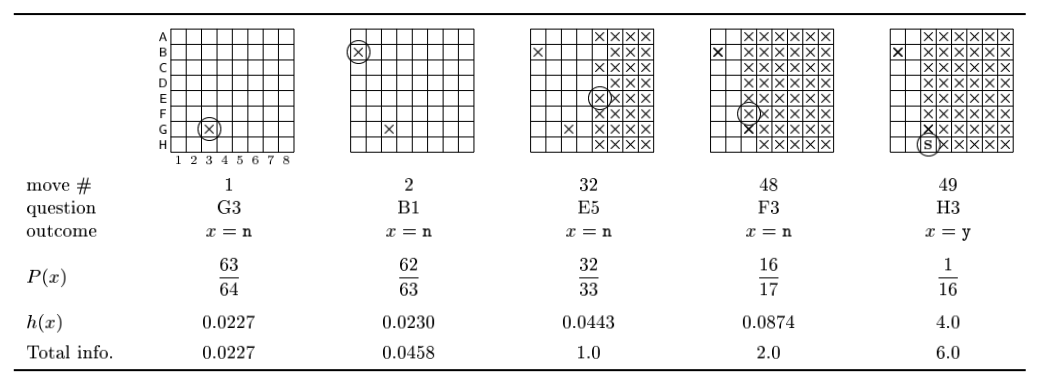
\includegraphics[width=0.9\linewidth]{img/submarines.png}
\end{figure*}

\begin{itemize}
    \item \textbf{Scenario 1:} You hit the submarine with the first question.
    \begin{itemize}
        \item You obtain \( \log(64) = 6 \) bit.
    \end{itemize}

    \item \textbf{Scenario 2:} You miss 32 times, then hit.
    \begin{itemize}
        \item The first miss gives you \( \log(64/63) = 0.0227 \) bit.
        \item By the 32\textsuperscript{nd} miss, you have
        \[
            \log(64/63) + \log(63/62) + \dots + \log(33/32) = 0.0227 + 0.0230 + \dots + 0.0444 = 1 \text{ bit}.
        \]
        \item The hit gives you \( \log(32) = 5 \) bit, for a total of 6 bit.
    \end{itemize}

    \item \textbf{General case:} You miss \( 64 - n \), then hit:
    \[
        \underbrace{\log \frac{64}{63} + \log \frac{63}{62} + \dots + \log \frac{n+1}{n}}_{\text{misses}} + \underbrace{\log \frac{n}{1}}_{\text{hit}} = \log 64 = 6 \text{ bit}
    \]

    \item \textbf{Conclusion:} Regardless of when you hit, you always get 6 bit.
\end{itemize}

\intuitb{Conclusions}{
\begin{itemize}
    \item For uniform distributions, \( h(x) \) corresponds to the length of the \textbf{binary representation} of \( x \) (i.e., number of yes/no questions).
    
    \item \( h(x) \) is a measure of the \textbf{“intrinsic”} information content of \( x \), regardless of how that information is obtained.
    
    \item Information is given by \textbf{probability mass exclusions} (Hartley 1928).
\end{itemize}

The goal of experiments is to \textbf{reduce uncertainty} about something by excluding possibilities. The takeaway is that you should design experiemtns with evenly probable outcomes to maximise information gain, as shown in Figure \ref{fig:entropy_coin}.
}

\section{Entropy in Continuous Distributions}

We have explored entropy in discrete RVs with finite alphabets, we then extend this to continuous RVs– by discretising the variable's continous domain.

\begin{itemize}
    \item We have a random variable \( X \in \mathbb{R} \) with PDF \( f(x) \).
    \item We use bins of width \( \Delta \) to get a discrete variable \( X^{\Delta} \) with
    \[
        p_i = \int_{(i - \frac{1}{2})\Delta}^{(i + \frac{1}{2})\Delta} f(x) \, dx = f(x_i) \Delta
    \]
    \item Now we take \( H(X^{\Delta}) \) as \( \Delta \to 0 \):
    \begin{align*}
        H(X^{\Delta}) &= -\sum p_i \log p_i \\
        &= -\sum f(x_i) \Delta \log(f(x_i) \Delta) \\
        &= -\sum \Delta f(x_i) \log f(x_i) - \log \Delta \\
        &= \underbrace{-\sum \Delta f(x_i) \log f(x_i)}_{\text{Riemann integral}}  \underbrace{- \log \Delta}_{\text{Divergent term}}
    \end{align*}
    \item Oh no, \( \lim_{\Delta \to 0} \log \Delta = -\infty \), so \( H(X^{\Delta}) \) diverges for any \( f(x) \).
    \item A foolproof strategy is to ignore $\log \Delta$ anyway, and define the \textbf{differential entropy} as:
\end{itemize}

\defb{Definition: Differential entropy}{
The \textit{differential entropy} of a continuous RV \( X \) with PDF \( f(x) \) is given by
\[
    H(X) := - \int f(x) \log f(x) \, dx
\]
}

\sn{Warning}{
The \( \log \Delta \) will come back to haunt us! Differential entropy lacks many interesting properties of discrete entropy. \bigskip 

\textbf{Disclaimer:} We may use the term ‘entropy’ for continuous RVs too.
}

\subsection{Properties of Differential Entropy}
Take an example of differential entropy in uniform distributions:
Let \( X \) be a uniform random variable in the interval of length \( a \).

\[
X \sim \mathcal{U}([0, a]) \quad \text{i.e.} \quad p(x) = \frac{1}{a}
\]

\[
H(X) = - \int_0^a \frac{1}{a} \log \frac{1}{a} \, dx = - \log \frac{1}{a} \int_0^a \frac{dx}{a} = \log a
\]

\textbf{Conclusions:} We see that Differential entropy:
\begin{itemize}
    \item Can be negative, e.g. for $a < 1$.
    \item Grows with the volume of the distribution $(2^{H(X)} = a > 0)$
\end{itemize}

\subsection{Surprisal in Gaussian Distributions}

\marginnote{\intuitsb{Modelling \ensuremath{x}}{We want to reduce surprisal to ensure we can compactly encode $x$ more efficiently. In this example, we want to model \( x \) with the Gaussian distribution. Reducing surprisal is then equivalent to reducing the prediction error, or the mean squared error (MSE). \bigskip

Try to imagine a distribution of $x$ and then we play around with the parameters of a Gaussian distribution to make it fit the distribution of $x$ better. \bigskip

If we find a more accurate $\mu$ for our model, we then reduce the MSE. And if our $\mu$ is already quite close to the true value of $x$, increasing precision (making reducing $\sigma$ to make the distribution more narrow, centring closer around $\mu$) can also sometimes reduce surprisal. However, if $\mu$ is too far from the true value of $x$, increasing precision can sometimes increase surprisal.}}

Let \( X \sim \mathcal{N}(\mu, \sigma^2) \) be a 1D Gaussian random variable, i.e.
\[
p(x) = \left( \sigma \sqrt{2 \pi} \right)^{-1} e^{-\frac{1}{2} \left( \frac{x - \mu}{\sigma} \right)^2}
\]


Then, surprisal is just the negative $ln$ of the PDF:
\[
h(x) = \ln \left( \sigma \sqrt{2 \pi} \right) + \frac{1}{2} \left( \frac{x - \mu}{\sigma} \right)^2
\]

This expression is equivalent to scaled mean squared error (MSE):
\[
h(x) = \ln \sigma + \frac{1}{2 \sigma^2} \text{MSE}(x, \mu) + C.
\]

If we predict \( x \) with a PDF \( \mathcal{N}(\mu, \sigma^2) \), we can lower the surprisal by:

\begin{itemize}
    \item Reducing the bias (i.e., moving \( \mu \) closer to \( x \)),
    \item (Sometimes) increasing the precision (i.e., increasing \( \sigma \)).
\end{itemize}


\subsection{Entropy in Gaussian Distributions}

We show that Entropy has a closed-form expression for Gaussian Distributions:

To calculate the entropy of a \(D\)-dimensional Gaussian distribution \(\mathcal{N}(\mu, \Sigma)\),

\[
p(x) = |2 \pi \Sigma|^{-1/2} \exp \left( -\frac{1}{2} (x - \mu)^\top \Sigma^{-1} (x - \mu) \right).
\]

The entropy \(H(X)\) is given by:
\[
H(X) = - \int_{-\infty}^{+\infty} \mathcal{N}(x; \mu, \Sigma) \ln \mathcal{N}(x; \mu, \Sigma) \, dx.
\]

Expanding, we get:
\[
H(X) = \frac{1}{2} \mathbb{E}[\ln |2 \pi \Sigma|] + \frac{1}{2} \mathbb{E}[(x - \mu)^\top \Sigma^{-1} (x - \mu)].
\]

For the first term, \(\mathbb{E}[\ln |2 \pi \Sigma|] = \ln |2 \pi \Sigma|\).

For the second term:
\[
\mathbb{E} \left[ (x - \mu)^\top \Sigma^{-1} (x - \mu) \right] = \operatorname{tr} \left( \Sigma^{-1} \mathbb{E} \left[ (x - \mu)(x - \mu)^\top \right] \right) = \operatorname{tr}(\Sigma^{-1} \Sigma) = D.
\]

Substituting back, we get:
\[
H(X) = \frac{1}{2} \ln |2 \pi \Sigma| + \frac{1}{2} D = \frac{1}{2} \ln \left( |2 \pi \Sigma| e^D \right).
\]

Overall:
\[
H(X) = \frac{1}{2} \ln |2 \pi e \Sigma|.
\]

\subsection{Takeaways of Entropy}
\begin{itemize}
    \item Entropy quantifies the \textbf{average information content} of an observation \(x\).
    \item Entropy serves as a \textbf{generalised variance} (e.g., measures predictability of \(X\)).
    \item For discrete distributions:
    \begin{itemize}
        \item Entropy is \textbf{bounded}: \(0 \leq H(X) \leq \log |\mathcal{X}|\).
        \item Related to the \textbf{number of yes/no questions} needed to determine \(x\).
    \end{itemize}
    \item For continuous distributions, \textbf{differential entropy} is defined, but can be negative and lacks some properties of discrete entropy.
\end{itemize}

\section{Source Coding Theorem}

\defb{Definition: Code and Code Length}{
    Given a random variable \( X \) with alphabet \( \mathcal{X} \) and an alphabet \( \mathcal{D} \), a \textbf{code} is a mapping
    \[
        C : \mathcal{X} \to \mathcal{D}^*,
    \]
    where \( \mathcal{D}^* \) is the set of all finite-length strings of symbols in \( \mathcal{D} \).

    The quantity \( \ell(x) \) is the \textbf{code length} of \( C(x) \), and \( L = \mathbb{E}[\ell(x)] \) the \textbf{average code length}.
}

\begin{itemize}
    \item For each symbol \( x \), the string \( C(x) \in \mathcal{D}^* \) is called a \textbf{codeword}.
    \item When \( |\mathcal{D}| = 2 \), \( C \) is a \textbf{binary code}. When \( |\mathcal{D}| = d \), \( C \) is a \textbf{d-ary code}.
\end{itemize}

Here are two example codes for the alphabet \( \mathcal{X} = \{ \text{a}, \text{b}, \text{c}, \text{d} \} \).

\begin{table}[h]
    \centering
    \begin{tabular}{c@{\hskip 1cm}c}
        \begin{tabular}{cc}
            \toprule
            \multicolumn{2}{c}{Binary} \\
            \midrule
            \( x \) & \( C(x) \) \\
            \midrule
            a & 00 \\
            b & 01 \\
            c & 10 \\
            d & 11 \\
            \bottomrule
        \end{tabular}
        &
        \begin{tabular}{cc}
            \toprule
            \multicolumn{2}{c}{Ternary} \\
            \midrule
            \( x \) & \( C(x) \) \\
            \midrule
            a & 0 \\
            b & 1 \\
            c & 2 \\
            d & 200 \\
            \bottomrule
        \end{tabular}
    \end{tabular}
\end{table}


\subsection{Coding for the Uniform Distribution}

\begin{itemize}
    \item We’ve seen that (in uniform distributions), entropy corresponds to the number of \textbf{yes/no} questions needed to guess \( x \).
    
    \[
    \begin{array}{c@{\quad\Rightarrow\quad}c@{\quad}c@{\quad\Rightarrow\quad}c}
        35 & 100011 & 6 & 000110 \\
        0 & 000000 & 17 & 010001 \\
        42 & 101010 & \dots & \dots \\
    \end{array}
    \]

    \item This forms a \textbf{binary code} for \( X \) with length
    \[
        L = H(X) = \log |\mathcal{X}|.
    \]

    \item More generally, \( \log |\mathcal{X}| \) is referred to as the \textbf{raw bit content} of \( X \).
\end{itemize}

\sn{Warning: Ceiling and the “Extra Bit”}{
    When \( |\mathcal{X}| \) is not a power of two, we may need an “extra bit” to encode symbols. You may see this written as \( L = \lceil \log |\mathcal{X}| \rceil \) or \( L = \log |\mathcal{X}| + 1 \).
}


\subsection{Non-uniform Distributions}

What happens when the distribution isn’t uniform?



\begin{itemize}
    \item \textbf{Example}: compressing Wikipedia, which has alphabet \( \mathcal{X} = \mathcal{E} \cup \mathcal{U} \):
    \begin{itemize}
        \item \( \mathcal{E} \) is the English alphabet, \( |\mathcal{E}| = 26 \);
        \item \( \mathcal{U} = \{ !, @, \#, \$, \%, -, \&, *, (, ) \} \) includes some unicode characters.
    \end{itemize}

    \item Assume that 98\% of Wikipedia content comes from \( \mathcal{E} \), and 2\% from \( \mathcal{U} \).

    \item A naive binary code of \( \mathcal{X} \) would require \( \lceil \log |\mathcal{X}| \rceil = \lceil \log 36 \rceil = 6 \) bits.

    \item \textbf{But}... if we ignore \( \mathcal{U} \), we can encode in \( \lceil \log |\mathcal{E}| \rceil = \lceil \log 26 \rceil = 5 \) bits.
\end{itemize}

\sn{Reduction in Code Length}{
    We have \textbf{reduced the code length} with only \textbf{2\% error}, simply by refusing to encode the minority of rarely-used symbols. And this generally would not have a major impact on the readability of the text– most information could still be conveyed.
}


\subsection{Law of Large Numbers}

The Law of Large Numbers states that as the number of independent, identically distributed (i.i.d.) random variables increases, their sample average converges to the expected value. This result forms a cornerstone of probability and statistics, establishing that with a large enough sample size, we can expect the sample mean to approximate the population mean closely.

\begin{itemize}
    \item Let \( Y^n = \frac{1}{n} \sum_{i=1}^n X_i \) be the mean of \(n\) i.i.d. random variables \( X_1, \dots, X_n \), with
    \[
    \mathbb{E}[X_1] = \dots = \mathbb{E}[X_n] = \mu \quad \text{and} \quad \operatorname{Var}(X_i) = \dots = \operatorname{Var}(X_n) = \sigma^2.
    \]

    \item By direct calculation, it can be shown that:
    \[
    \mathbb{E}[Y^n] = \mu \quad \text{and} \quad \operatorname{Var}(Y^n) = \frac{\sigma^2}{n}.
    \]

    \item As \( n \to \infty \), \( Y^n \) has \textbf{vanishing variance}, meaning \( Y^n \) becomes increasingly close to \( \mu \).
\end{itemize}

\thm{Weak Law of Large Numbers}{
    Let \( Y^n = \frac{1}{n} \sum_{i=1}^n X_i \). As \( n \to \infty \), \( Y^n \) converges in probability to \( \mu \):
    \[
    Y^n \xrightarrow{P} \mu, \quad \text{that is,} \quad \lim_{n \to \infty} \Pr\left( |Y^n - \mu| < \varepsilon \right) = 1
    \]
    for any \( \varepsilon > 0 \).
}

\chapter{Symbol Codes}


Previously, we proved that there exists a mapping from \( X^n \) to \( \mathcal{D}^* \) which, with high probability, shortens strings (specifically to lengths shorter than \( n \log |\mathcal{X}| \)).\bigskip

However, this approach is impractical for software implementation because:
\begin{itemize}
    \item It only works for infinitely large blocks.
    \item It requires enumerating all \( 2^{nH} \) elements in the typical set.
\end{itemize}

This is where \textit{symbol codes} come into play.

\section{The Problem of Coding}

% \marginnote{\defsb{Old Definition: Code Length}{Given a random variable \( X \) with alphabet \( \mathcal{X} \) and an alphabet \( \mathcal{D} \), a \textbf{code} is a mapping 
% \[
% C : \mathcal{X} \rightarrow \mathcal{D}^*,
% \]
% where \( \mathcal{D}^* \) is the set of all finite-\textbf{length} strings of symbols in \( \mathcal{D} \). \bigskip

% The quantity \( \ell(x) \) is the \textbf{code length} of \( C(x) \), and \( L = \mathbb{E}[\ell(x)] \) is the average \textbf{code length}.}}


\defb{Definition: Code and Code Length}{
    Given a random variable \( X \) with alphabet \( \mathcal{X} \) and an alphabet \( \mathcal{D} \), a \textit{code} is defined as a mapping
    \[
        C : \mathcal{X} \rightarrow \mathcal{D}^*,
    \]
    where \( \mathcal{D}^* \) is the set of all finite-length strings of symbols in \( \mathcal{D} \). \bigskip

    The code length of \( C(x) \) for a symbol \( x \in \mathcal{X} \) is denoted \( \ell(x) \), and the \textit{average code length} is defined as
    \[
        L = \mathbb{E}[\ell(x)].
    \]
    We can use the shorthand notation \( \ell_i := \ell(x_i) \) and \( D := |\mathcal{D}| \) for convenience.}

\subsubsection{Example: Morse Code}
Morse Code maps each letter in the English alphabet to a binary string using dots and dashes.
\begin{center}
    \begin{tabular}{>{\bfseries}c c @{\hspace{1.5cm}} >{\bfseries}c c @{\hspace{1.5cm}} >{\bfseries}c c}
        A & \textbullet{} --                                        & J & \textbullet{} -- -- --                       & S & \textbullet{} \textbullet{} \textbullet{}    \\
        B & -- \textbullet{} \textbullet{} \textbullet{}            & K & -- \textbullet{} --                          & T & --                                           \\
        C & -- \textbullet{} -- \textbullet{}                       & L & \textbullet{} -- \textbullet{} \textbullet{} & U & \textbullet{} \textbullet{} --               \\
        D & -- \textbullet{} \textbullet{}                          & M & -- --                                        & V & \textbullet{} \textbullet{} \textbullet{} -- \\
        E & \textbullet{}                                           & N & -- \textbullet{}                             & W & \textbullet{} -- --                          \\
        F & \textbullet{} \textbullet{} -- \textbullet{}            & O & -- -- --                                     & X & -- \textbullet{} \textbullet{} --            \\
        G & -- -- \textbullet{}                                     & P & \textbullet{} -- -- \textbullet{}            & Y & -- \textbullet{} -- --                       \\
        H & \textbullet{} \textbullet{} \textbullet{} \textbullet{} & Q & -- -- \textbullet{} --                       & Z & -- -- \textbullet{} \textbullet{}            \\
        I & \textbullet{} \textbullet{}                             & R & \textbullet{} -- \textbullet{}               &   &                                              \\
    \end{tabular}
\end{center}
\subsubsection{Desiderata of Good Codes}
A well-designed code should:
\begin{enumerate}
    \item Be short (i.e., use few bits per symbol).
    \item Be easily decodable (i.e., invertible with ease).
\end{enumerate}

The key question in data compression is: \textit{How short can a code be while still being decodable?}

\section{No Free Lunch for Information Theorists}

\subsection{Compression Limitations}
Let \( \mathcal{A}_L \) denote the set of all strings of length \( L \). Consider a compressor \( C : \mathcal{A}_L \rightarrow \mathcal{A}^* \). \bigskip

Can there be a compressor that shortens all strings in \( \mathcal{A}_L \)?\bigskip

\marginnote{
    \defsb{No Free Lunch Theorem}{There cannot exist a compressor that shortens all strings in \( \mathcal{A}_L \).}
}

The answer is no. There are two outcomes– if a compressor is:
\begin{itemize}
    \item \textit{Invertible}, then some strings will be lengthened.
    \item \textit{Not invertible}, it loses information.
\end{itemize}
Thus, compression must balance between lossless and lossy encoding.

\subsection{Types of Data Compression}

Due to the \textbf{no free lunch} theorem, we are left with two primary types of data compression:

\begin{itemize}
    \item \textbf{Lossy Compression}: The compressor reduces the size of most strings, but some strings are mapped to the same encoding, which leads to a loss of the original information.

    \item \textbf{Lossless Compression}: The compressor shortens most strings, but it must lengthen some others to ensure all information is retained.
\end{itemize}

\sn{Aside: Proofs of the Source Coding Theorem}{
    \begin{itemize}
        \item C\&T (Cover and Thomas) and our course notes proved the \textbf{Source Coding Theorem (SCT)} using the Asymptotic Equipartition Property (AEP) with a \textbf{lossless encoder}. In this approach, all strings \( x^n \) are uniquely mapped, with some codewords being short (for \( x^n \in A^{(n)}_\epsilon \)) and others long (for \( x^n \notin A^{(n)}_\epsilon \)).

        \item MacKay's approach to proving SCT also relies on AEP but uses a \textbf{lossy encoder}. Here, only strings in \( A^{(n)}_\epsilon \) are encoded, while other strings result in errors. However, the probability of such errors is very small.
    \end{itemize}

    In both approaches, the SCT holds– which means we can achieve efficient coding either way.
}

\subsection{A Decoder's Life is Hard}

Consider the following example: given two prime numbers \( a \) and \( b \), a code \( C \) could map the pair \( (a, b) \) to the binary encoding of their product \( a \cdot b \).

\[C(a,b) = \text{binary encoding of } a \cdot b\]\marginnote[-100pt]{This is an example of RSA encryption. Take two primes, $a = 13$ and $b = 17$. The product is $a \cdot b = 221$. The binary encoding of 221 is 11011101. Assuming we work only with primes (because if we don't, the code is not invertible), it would take a lot of effort to find out the original prime factorisation of 221.}

By the \textbf{prime factorisation theorem}, this code is invertible, meaning that the original values \( a \) and \( b \) can be recovered from \( C(a, b) \). However, decoding requires prime factorisation, which is computationally challenging. \footnote{(In general, there is a bit of a trade-off: the more work the encoder does, the less the decoder needs to do. We won’t get to see this, as it applies only to more sophisticated channel codes.)}

\hl{
    Even if a code is theoretically invertible, it may not be practical to decode. There is often a trade-off between the encoding and decoding complexity: the more work the encoder does, the less the decoder may need to do.
}


\section{Types of Code}
\defb{Definition: Nonsingular Code}{
    A code is called \textbf{nonsingular} if each symbol maps to a unique codeword, i.e., for any two symbols \( x \neq x' \), we have \( C(x) \neq C(x') \). This property ensures that the code is invertible at the level of individual codewords. \bigskip

    \textbf{Example:}
    \bigskip


    \begin{tabular}{p{0.45\textwidth} p{0.45\textwidth}}
        \begin{tabular}{cc}
            \toprule
            \multicolumn{2}{c}{\textbf{Nonsingular Code}} \\
            \midrule
            \( x \) & \( C(x) \)                          \\
            \toprule
            \( a \) & 000                                 \\
            \( b \) & 001                                 \\
            \( c \) & 010                                 \\
            \bottomrule
        \end{tabular}
         &
        \begin{tabular}{cc}
            \toprule
            \multicolumn{2}{c}{\textbf{Singular Code}} \\
            \midrule
            \( x \) & \( C(x) \)                       \\
            \toprule
            \( a \) & 0                                \\
            \( b \) & 0                                \\
            \( c \) & 1                                \\
            \bottomrule
        \end{tabular} \\
    \end{tabular}
}

\marginnote{
    \defsb{Definition: Uniquely Decodable}{
    A code \( C \) is \textbf{uniquely decodable} if its extension \( C^* \) is nonsingular, meaning each sequence of symbols in \( \mathcal{X} \) maps to a unique sequence in \( \mathcal{D} \).
}
}

\marginnote{
    \ex{Nonsingular but not Uniquely Decodable: Morse Code}{
    Morse code is an example of a nonsingular code but not a uniquely decodable code. Without spaces or punctuation, some symbol sequences are ambiguous. For example:
    \[
        \text{``. -- . . --''} \rightarrow \text{`AU' or `EDT'}
    \]
}\label{ex:morse_code}
}

\defb{Definition: Extended Code}{
    Given a code \( C \), the \textbf{extended code} \( C^* : \mathcal{X}^+ \rightarrow \mathcal{D}^* \) is the code formed by concatenating codewords from \( C \):
    \[
        C^*(x_1 x_2 \dots x_n) = C(x_1) C(x_2) \dots C(x_n).
    \]

    \bigskip
    \textbf{Example:}
    Suppose we have a code \( C \) with the following mappings:
    \[
        C(a) = 0, \quad C(b) = 10, \quad C(c) = 11.
    \]
    Then, for the sequence \( x = abc \), the extended code \( C^*(abc) \) is given by:
    \[
        C^*(abc) = C(a)C(b)C(c) = 0 \, 10 \, 11 = 01011.
    \]
}






\ex{Nonsingular and Uniquely Decodable Code}{
    Consider the following code \( C \) for the alphabet \( \{a, b, c\} \):
    \[
        C(a) = 0, \quad C(b) = 01, \quad C(c) = 11.
    \]

    This code is nonsingular because each symbol maps to a unique codeword (no two symbols share the same codeword).

    It is also uniquely decodable because any sequence of codewords can be decoded unambiguously. For example, given the encoded message \( 001110 \):
    \[
        001110 \rightarrow C(a)C(b)C(c)C(a) = abca.
    \]

    No alternative sequence of symbols could produce the same encoding, so we have unique decodability. That brings us to the next type of code: prefix codes.
}


\defb{Definition: Prefix Code}{
    A \textbf{prefix code} (also known as a prefix-free or instantaneous code) is a code in which no codeword is the prefix of any other codeword. This property allows for immediate decoding as soon as each codeword is received, making it highly efficient. \bigskip

    \textbf{Example:}

    An example of a prefix code for a binary alphabet \( \mathcal{D} = \{0, 1\} \):
    \[
        \begin{array}{cc}
            \toprule
            x & C(x) \\
            \midrule
            a & 0    \\
            b & 10   \\
            c & 110  \\
            \bottomrule
        \end{array}
    \]

    In this code, no codeword is a prefix of another, allowing for unambiguous decoding. Prefix codes are widely used in data compression due to their efficient and instantaneous decoding properties. They can be represented as trees, with each branch representing a symbol and each leaf representing a complete codeword.
}





\begin{figure}[h]
    \centering
    \begin{tikzpicture}[scale=1]
        % Define colors
        \definecolor{outer}{RGB}{248, 249, 250}
        \definecolor{middle1}{RGB}{230, 240, 249}
        \definecolor{middle2}{RGB}{191, 219, 254}
        \definecolor{inner}{RGB}{147, 197, 253}

        % Draw circles from outermost to innermost
        \fill[outer] (0,0) circle (4cm);
        \draw[thick] (0,0) circle (4cm);

        \fill[middle1] (0,0) circle (3cm);
        \draw[thick] (0,0) circle (3cm);

        \fill[middle2] (0,0) circle (2cm);
        \draw[thick] (0,0) circle (2cm);

        \fill[inner] (0,0) circle (1cm);
        \draw[thick] (0,0) circle (1cm);

        % Add labels with proper syntax
        \node[align=center, font=\small] at (0, -0) {\textbf{All Codes}};
        \node[align=center, font=\small] at (0, 1.4) {\textbf{Prefix Codes}};
        \node[align=center, font=\small] at (0, 2.45) {\textbf{Uniquely}\\ \textbf{Decodable Codes}};
        \node[align=center, font=\small] at (0, 3.4) {\textbf{Nonsingular Codes}};   \end{tikzpicture}
    \caption{Hierarchy of different types of codes}
    \label{fig:code-hierarchy}
\end{figure}

\subsection{Prefix Codes}

\textbf{Prefix codes} are codes in which no codeword is the prefix of any other codeword. This property allows for \textbf{instantaneous decoding}—each codeword can be uniquely identified as soon as it is fully received, making it efficient for communication and compression applications. \bigskip

Below are two examples for a binary code \( \mathcal{D} = \{0, 1\}, D = 2 \):

\begin{figure*}
    \centering

    \begin{minipage}{0.4\textwidth}
        \centering
        \begin{tabular}{cc}
            \toprule
            \( x \) & \( C(x) \) \\
            \midrule
            \( a \) & 0          \\
            \( b \) & 100        \\
            \( c \) & 11         \\
            \bottomrule
        \end{tabular}
    \end{minipage}
    \hspace{2cm}
    \begin{minipage}{0.4\textwidth}
        \centering
        \begin{tabular}{cc}
            \toprule
            \( x \) & \( C(x) \) \\
            \midrule
            \( a \) & 00         \\
            \( b \) & 01         \\
            \( c \) & 10         \\
            \( d \) & 11         \\
            \bottomrule
        \end{tabular}
    \end{minipage}

    \bigskip



    \begin{minipage}{0.4\textwidth}
        \centering
        \begin{tikzpicture}[level distance=1.5cm,
                level 1/.style={sibling distance=3cm},
                level 2/.style={sibling distance=1.5cm}]

            % First tree example
            \node (Root1) {Root}
            child {node [label=below:\textbf{0 = a}] {0}} % direct leaf for a
            child {node {1}
                    child {node {0}
                            child {node [label=below:\textbf{100 = b}] {0}}}
                    child {node [label=below:\textbf{11 = c}] {1}}};
        \end{tikzpicture}
    \end{minipage}
    \hspace{2cm}
    \begin{minipage}{0.4\textwidth}
        \centering
        \begin{tikzpicture}[level distance=1.5cm,
                level 1/.style={sibling distance=3cm},
                level 2/.style={sibling distance=1.5cm}]

            % Second tree example
            \node (Root2) {Root}
            child {node {0}
                    child {node [label=below:\textbf{00 = a}] {0}}
                    child {node [label=below:\textbf{01 = b}] {1}}}
            child {node {1}
                    child {node [label=below:\textbf{10 = c}] {0}}
                    child {node [label=below:\textbf{11 = d}] {1}}};
        \end{tikzpicture}
    \end{minipage}
\end{figure*}

\bigskip
\subsubsection{Limits of Prefix Codes}

Prefix codes have constraints related to the structure of the tree. Two key observations are:

\begin{itemize}
    \item A \textbf{complete tree} with \( D^{\ell_{\max}} \) codewords (where \( \ell_{\max} \) is the length of the longest codeword) is fully populated, meaning each branch has reached a leaf at that level.
    \item An \textbf{incomplete tree} has some shorter codewords, reducing the total number of available codewords.
\end{itemize}

Intuitively, adding a new codeword consumes all potential branches (or descendants) that would otherwise be available for longer codewords.

\sn{Key Insight for Prefix Codes}{
    Prefix codes provide efficiency in decoding by ensuring no codeword is a prefix of another– so we do not need a separation character as seen in the Morse Code Example  \ref{ex:morse_code}. However, this comes at the expense of limiting the code length options, as adding a codeword shortens the tree depth for all other codewords.
}


\section{Kraft Inequality}

\thm{Kraft Inequality}{
    The codeword lengths \(\ell_i\) of any \(D\)-ary prefix code must satisfy the inequality:
    \[
        \sum_{i} D^{-\ell_i} \leq 1
    \]
    Conversely, given any set of lengths that satisfy this inequality, there exists a corresponding prefix code.
    \paragraph{Proof:}
    \begin{itemize}
        \item A tree representing a prefix code with the longest codeword length \(\ell_{\text{max}}\) can have at most \(D^{\ell_{\text{max}}}\) leaves.
        \item Each codeword of length \(\ell_i\) corresponds to \(D^{\ell_{\text{max}} - \ell_i}\) descendants at level \(\ell_{\text{max}}\).
        \item Summing over all codewords, the inequality becomes:
              \[
                  \sum_{i} D^{\ell_{\text{max}} - \ell_i} \leq D^{\ell_{\text{max}}} \Rightarrow \sum_{i} D^{-\ell_i} \leq 1
              \]
    \end{itemize}
}


\subsection{Interpretation: Codeword Supermarket}

To illustrate the Kraft inequality, consider the following interpretation. Imagine a “codeword supermarket” where shorter codewords are “more expensive,” and we are constrained by a maximum budget. The inequality \(\sum_i D^{-\ell_i} \leq 1\) reflects the idea that the budget cannot be exceeded.

\begin{marginfigure}[30pt]
    \centering

    \begin{tabular}{|c|c|c|c|l|}
        \hline
        \multirow{8}{*}{0} & \multirow{4}{*}{00} & 000                  & 0000 & \multirow{16}{*}{\rotatebox{90}{The total symbol code budget}} \\
        \cline{3-4}
                           &                     & 001                  & 0001 &                                                                \\
        \cline{3-4}
                           &                     & \multirow{2}{*}{001} & 0010 &                                                                \\
        \cline{4-4}
                           &                     &                      & 0011 &                                                                \\
        \cline{2-4}
                           & \multirow{4}{*}{01} & \multirow{2}{*}{010} & 0100 &                                                                \\
        \cline{4-4}
                           &                     &                      & 0101 &                                                                \\
        \cline{3-4}
                           &                     & \multirow{2}{*}{011} & 0110 &                                                                \\
        \cline{4-4}
                           &                     &                      & 0111 &                                                                \\
        \cline{1-4}
        \multirow{8}{*}{1} & \multirow{4}{*}{10} & \multirow{2}{*}{100} & 1000 &                                                                \\
        \cline{4-4}
                           &                     &                      & 1001 &                                                                \\
        \cline{3-4}
                           &                     & \multirow{2}{*}{101} & 1010 &                                                                \\
        \cline{4-4}
                           &                     &                      & 1011 &                                                                \\
        \cline{2-4}
                           & \multirow{4}{*}{11} & \multirow{2}{*}{110} & 1100 &                                                                \\
        \cline{4-4}
                           &                     &                      & 1101 &                                                                \\
        \cline{3-4}
                           &                     & \multirow{2}{*}{111} & 1110 &                                                                \\
        \cline{4-4}
                           &                     &                      & 1111 &                                                                \\
        \hline
    \end{tabular}

    \caption{visualisation of the Codeword Supermarket}
\end{marginfigure}

\bigskip

\textbf{Note:} While this inequality has been demonstrated for prefix codes, the theorem extends to uniquely decodable codes as well (see MacKay Sec. 5.2 and C\&T Theorem 5.5.1 for further proof), where it guarantees the existence of a set of code lengths that satisfy the condition.

\section{Lagrange Multipliers for Optimal Code Length}

\thm{Theorem: Lagrange Multiplier}{
    Consider a constrained optimisation problem:
    \[
        \min f(\mathbf{x}) \quad \text{subject to} \quad g(\mathbf{x}) = 0
    \]
    where \( \mathbf{x} \in \mathbb{R}^k \), \( f : \mathbb{R}^k \to \mathbb{R} \) is the objective function, and \( g : \mathbb{R}^k \to \mathbb{R}^c \) is the constraint function. \bigskip

    The Lagrangian function for this optimisation problem is defined as:
    \[
        L := f(\mathbf{x}) + \boldsymbol{\lambda} \cdot g(\mathbf{x})
    \]
    where \(\boldsymbol{\lambda}\) represents the Lagrange multipliers. Any local extremum of \( f(\mathbf{x}) \) subject to \( g(\mathbf{x}) = 0 \) satisfies \( \nabla_{\mathbf{x}, \boldsymbol{\lambda}} L = 0 \).
}

In practice, solving a \( k \)-dimensional optimisation problem with \( c \) constraints involves finding \( k + c \) equations as follows:
\begin{itemize}
    \item \( k \) equations for \( x_1, \ldots, x_k \):
          \[
              \frac{dL}{dx_1} = 0, \, \ldots, \, \frac{dL}{dx_k} = 0
          \]
    \item \( c \) equations for \(\lambda_1, \ldots, \lambda_c\):
          \[
              g_1(x) = 0, \, \ldots, \, g_c(x) = 0
          \]
\end{itemize}

\subsection{Optimal Codes}

\hl{How good is the best prefix code for a given $p_i$?}

The objective is to find the best prefix code for a given distribution \( p_i \) by minimising the expected code length:
\[
    \min \sum_i p_i \ell_i \quad \text{subject to} \quad \sum_i D^{-\ell_i} = 1
\]
Using Lagrange multipliers, we define the Lagrangian: \marginnote{
    We make two assumptions: that $l_i$ is continuous, and that the equality constraint is satisfied.}

\[
    L = \sum_i p_i \ell_i + \lambda \left( \sum_i D^{-\ell_i} - 1 \right)
\]

\begin{enumerate}
    \item Differentiate the Lagrangian with respect to \(\ell_i\) and set to 0:
          \[
              \frac{dL}{d\ell_i} = p_i - \lambda D^{-\ell_i} \ln D = 0
          \]
    \item Solve for \(\ell_i\):
          \[
              D^{-\ell_i} = \frac{p_i}{\lambda \ln D}
          \]
    \item Substitute into the Kraft inequality and solve for \(\lambda\):
          \[
              \sum_i D^{-\ell_i} = 1 \Rightarrow \frac{1}{\lambda \ln D} = 1 \Rightarrow \lambda = \frac{1}{\ln D}
          \]
    \item Substitute \(\lambda\) back to obtain the optimal code length:
          \[
              \ell_i^* = -\log_D p_i
          \]
    \item Take the second derivative of the Lagrangian:
          \[
              \frac{d^2L}{d\ell_i^2} = D^{-\ell_i} \ln D \geq 0
          \]
          Since this derivative is non-negative and there is only one solution to \( \frac{dL}{d\ell_i} = 0 \), this solution is a global minimum.
\end{enumerate}

\defb{Entropy is the Optimal Code Length}{
    Thus, the average length of the optimal code is:
    \[
        L^* = \sum_i p_i \ell_i^* = -\sum_i p_i \log_D p_i = H_D(X)
    \]
    which shows that the entropy \( H(X) \) represents the minimum average code length.
}


The above results reveal a duality between probability distributions (PDFs) and prefix codes:
\begin{itemize}
    \item Given a PDF \( p_i \), there exists an optimal code \( C \) with code lengths \( \ell_i = -\log_D p_i \).
    \item Given a set of Kraft-compatible lengths \( \ell_i \), there exists a PDF \( p_i \propto D^{-\ell_i} \) for which these lengths are optimal.
\end{itemize}

These implicit probabilities \( p_i \) are sometimes called the \textbf{implicit probabilities} of the code \( C \).

\section{Huffman Coding}

\thm{Algorithm: Huffman Coding}{
    Huffman coding provides an optimal encoding strategy for a given set of symbols with associated probabilities. The algorithm works as follows:
    \begin{enumerate}
        \item Select the two symbols with the smallest probabilities.
        \item Combine these two symbols into a single "node" and assign it a probability equal to the sum of the original two.
        \item Repeat the above steps until only one node remains.
    \end{enumerate}

    Huffman coding is optimal. That is, if \( C^* \) is the Huffman code and \( C' \) is any other uniquely decodable code, then \( L(C^*) \leq L(C') \).

    \paragraph{Proof: } The proof is complicated, see MacKay, Exercise 5.16, or Cover and Thomas, Sec. 5.8.
}


\subsection{Huffman Coding Example}

Consider an example with symbol set \( X = \{a, b, c, d, e\} \) and probabilities \( p = \{0.25, 0.25, 0.2, 0.15, 0.15\} \).

\begin{figure}

    \centering
    \begin{tikzpicture}[level distance=1.5cm,
            level 1/.style={sibling distance=3.5cm},
            level 2/.style={sibling distance=2cm},
            level 3/.style={sibling distance=1.75cm}]

        % Right-side tree
        \node (Root2) {Root}
        child {node {0}
                child {node [label=below:\textbf{00 = a}] {0}}
                child {node {1}
                        child {node [label=below:\textbf{010 = d}] {0}}
                        child {node [label=below:\textbf{011 = e}] {1}}
                    }
            }
        child {node {1}
                child {node [label=below:\textbf{10 = b}] {0}}
                child {node [label=below:\textbf{11 = c}] {1}}
            };
    \end{tikzpicture}
    \caption{Huffman Tree Example}
\end{figure}




\begin{table}[h!]
    \centering
    \begin{tabular}{ccccc}
        \textbf{Symbol} & \textbf{Probability \( p_i \)} & \textbf{Length \( \ell_i \)} & \textbf{Code \( C(x) \)} \\
        \hline
        \( a \)         & 0.25                           & 2                            & 00                       \\
        \( b \)         & 0.25                           & 2                            & 10                       \\
        \( c \)         & 0.20                           & 2                            & 11                       \\
        \( d \)         & 0.15                           & 3                            & 010                      \\
        \( e \)         & 0.15                           & 3                            & 011                      \\
    \end{tabular}
    \caption{Huffman Coding Example}
\end{table}

In this example, the codewords are assigned by traversing the Huffman tree, with each branch representing either a 0 or a 1.

\sn{Interim Summary: Symbol Codes}{
    \begin{itemize}
        \item Symbol codes map each individual symbol onto a codeword.
        \item Prefix codes are those where no codeword is the start of another codeword, and they can be represented as trees.
        \item \textbf{Kraft inequality}: for prefix codes, \(\sum_{i} D^{-\ell_i} \leq 1\).
        \item \textbf{Source coding theorem for symbol codes}:
              \begin{itemize}
                  \item There exists a code that achieves a length close to \(H(X)\) (achievability).
                  \item There are no codes that achieve length \(< H(X)\) (converse).
              \end{itemize}
    \end{itemize}
}

\section{Using the Wrong Code}

\begin{itemize}
    \item So far, we have assumed a known PDF \( p(x) \) and built a code for it.
    \item What happens if we use the wrong code?

          \ex{Wrong Code}{
              Suppose we assume that the data \( X \) comes from a PDF \( q = \left\{\frac{1}{2}, \frac{1}{4}, \frac{1}{8}, \frac{1}{8}\right\} \) and create a code \( C = \{0, 10, 110, 111\} \) based on this assumption.
              \begin{itemize}
                  \item Expected average length: \( - \frac{1}{2} \log \frac{1}{2} - \frac{1}{4} \log \frac{1}{4} - 2 \times \frac{1}{8} \log \frac{1}{8} = 1.75 \) bits.
                  \item However, if the actual distribution is \( p = \{0, \frac{1}{3}, \frac{1}{3}, \frac{1}{3}\} \), the average length used would be:
                        \[ -0 \log \frac{1}{2} - \frac{1}{3} \log \frac{1}{4} - \frac{2}{3} \log \frac{1}{8} = 2.66 \text{ bits!} \]
                  \item Assuming the wrong distribution means we use more bits than necessary.
              \end{itemize}
          }

\end{itemize}
\marginnote{
    \defsb{Cross Entropy}{
        The cross-entropy of a PDF \( q \) relative to a PDF \( p \) is defined as:
        \[
            H(p, q) := -\sum_{x \in X} p(x) \log q(x)
        \]
        Cross-entropy represents the expected length of a code optimised for \( q(x) \) when applied to samples from \( p(x) \).
    }
}
Mathematically, we can describe the difference in performance as follows:
\begin{itemize}
    \item Consider two random variables on the same alphabet \( X \), with PDFs \( p(x) \) and \( q(x) \).
    \item The optimal code for \( q(x) \) has lengths \( \ell(x) = -\log q(x) \).
    \item When used to compress samples from \( p(x) \), the average length is:
          \[ L(p, q) = \sum_{x \in X} p(x) \ell(x) = -\sum_{x \in X} p(x) \log q(x) \]
\end{itemize}



\section{Kullback-Leibler Divergence}

\defb{Kullback-Leibler Divergence}{
    The Kullback-Leibler (KL) divergence, also known as relative entropy, of two PDFs \( p \) and \( q \) on \( X \) is given by:
    \[
        D_{\text{KL}}(p \parallel q) := \sum_{x \in X} p(x) \log \frac{p(x)}{q(x)}
    \]
    KL divergence measures the "difference" between two distributions.
}

\begin{itemize}
    \item \textbf{Interpretation:} KL divergence quantifies the expected "extra cost" incurred when using a code optimised for \( q \) to compress data that actually follows \( p \).
    \item \textbf{Cross-Entropy Decomposition:}
          \[
              D_{\text{KL}}(p \parallel q) = H(p, q) - H(p)
          \]
          Here, \( H(p, q) \) is the cross-entropy, representing the expected length of the \( q \)-optimal code on \( p \), and \( H(p) \) is the expected length of the \( p \)-optimal code on \( p \).
\end{itemize}
\marginnote{Gibbs' Inequality is extremely important!}

\thm{Gibbs' Inequality}{
    KL divergence is always non-negative:
    \[
        D_{\text{KL}}(p \parallel q) \geq 0
    \]
    Equality holds if and only if \( p(x) = q(x) \) for all \( x \in X \).

    \paragraph{Proof}
    \begin{itemize}
        \item Start with the negative KL divergence:
              \[
                  -D_{\text{KL}}(p \parallel q) = \sum_{x \in \mathcal{X}} p(x) \log \frac{q(x)}{p(x)}
              \]
        \item Using Jensen's inequality, given the concave-down $\cap$ property of the log function:
              \[
                  -D_{\text{KL}}(p \parallel q) \leq \log \sum_{x \in \mathcal{X}} p(x) \frac{q(x)}{p(x)} = \log \sum_{x \in \mathcal{X}} q(x) = \log 1 = 0
              \]
              This leads to the desired result: \( D_{\text{KL}}(p \parallel q) \geq 0 \).
    \end{itemize}

    \paragraph{Proof of Equality condition $(=)$}
    \begin{itemize}
        \item If \( p(x) = q(x) \) for all \( x \in \mathcal{X} \), then:
              \[
                  D_{\text{KL}}(p \parallel q) = \sum_{x \in \mathcal{X}} p(x) \log \frac{p(x)}{p(x)} = \sum_{x \in \mathcal{X}} p(x) \cdot 0 = 0
              \]
              Conversely, since KL is convex in \( q \), it has a unique global minimum, so \( D_{\text{KL}}(p \parallel q) = 0 \) if and only if \( p = q \).
    \end{itemize}


}

\subsection{Properties of KL Divergence}
\begin{itemize}
    \item Why is KL a “divergence”? Let’s consider a \textit{geometric interpretation}.
    \item Due to the convexity of the log function, \( D_{\text{KL}}(p \parallel q) \) is convex in \( q \).
    \item Consider a distribution at a middle point \( \lambda \) between \( p \) and \( q \):
          \begin{align*}
              D_{\text{KL}}\big(p \parallel \lambda q + (1 - \lambda)p\big) & \leq \lambda D_{\text{KL}}(p \parallel q) + (\lambda-1 )\underbrace{D_{\text{KL}}(p \parallel p)}_{= 0} \\
                                                                            & = \lambda D_{\text{KL}}(p \parallel q)
          \end{align*}
\end{itemize}

\begin{center}
    \begin{tikzpicture}
        % Draw curved background
        \draw[thick, fill=gray!10] plot[smooth cycle, tension=0.7] coordinates {(-1,2) (1.5,1.5) (2,-1) (0.5,-2.5) (-2,-1.5)};

        % Draw point p
        \node[circle, fill=black, inner sep=1pt, label=above:$p$] (p) at (0,0) {};

        % Draw point q
        \node[draw=none, inner sep=1pt, label=below:$q$] (q) at (1.35,-1.35) {};

        \node[circle, fill= black, inner sep=1pt, label=right:$\lambda$] (lambda) at (0.675, -0.675) {};

        % Arrows diverging from p
        \draw[->, thick] (p) -- (0.8, 0.8);
        \draw[->, thick] (p) -- (1.35, -1.35);
        \draw[->, thick] (p) -- (0, -1);
        \draw[->, thick] (p) -- (-0.8, -0.2);
        \draw[->, thick] (p) -- (-1, 1);


        % Label for the curved region
    \end{tikzpicture}
\end{center}

\begin{itemize}
    \item The further away you go from \( p \), the larger \( D_{\text{KL}} \) grows.
\end{itemize}

\subsection{KL Divergence as a measure of Entropy}
\marginnote{
    \intuitsb{KL Divergence can be Infinite}{
        If \( q(x) = 0 \) and \( p(x) > 0 \) for any \( x \), then \( D_{\text{KL}}(p \parallel q) = \infty \). \bigskip


        KL becomes infinite if \( p \) contains symbols or events that are not accounted for in \( q \).

    }
}
\begin{itemize}
    \item Entropy can be interpreted as the negative of the KL divergence to a uniform distribution:
          \begin{align}
              D_{\text{KL}}(p \parallel u) & = \sum_i p_i \log \frac{p_i}{u_i} \notag                                                            \\
                                           & = -\sum_i p_i \log \frac{1}{p_i} - \underbrace{\sum_i p_i}_{=1} \log \frac{1}{|\mathcal{X}|} \notag \\
                                           & = -H(P) + \log |\mathcal{X}|
          \end{align}
    \item This property leads to a useful bound on entropy:
          \[
              H(p) = \log |X| - D_{\text{KL}}(p \parallel u) \leq \log |X|
          \]
    \item KL divergence is not symmetric, which makes it unsuitable as a distance metric:
          \[
              D_{\text{KL}}(p \parallel q) \neq D_{\text{KL}}(q \parallel p)
          \]
    \item If \( q(x) = 0 \) and \( p(x) > 0 \) for any \( x \), then \( D_{\text{KL}}(p \parallel q) = \infty \).
\end{itemize}



\ex{Example: KL Divergence Calculations}{
    Given three distributions \( p_1, p_2, \) and \( p_3 \) over the symbols \( a, b, c, d \), with varying probabilities:
    \begin{center}
        % First chart (p1)
        \begin{tikzpicture}
            \begin{axis}[
                    ybar,
                    width=8cm,
                    height=4cm,
                    ymin=0, ymax=1,
                    bar width=15pt,
                    symbolic x coords={a, b, c, d},
                    xtick=data,
                    ylabel={$p_1$},
                    ytick={0, 0.25, 0.5, 0.75, 1},
                    nodes near coords,
                    every node near coord/.append style={font=\small},
                    enlargelimits=0.15,
                    ymajorgrids
                ]
                \addplot coordinates {(a, 0.25) (b, 0.25) (c, 0.25) (d, 0.25)};
            \end{axis}
        \end{tikzpicture}

        % Second chart (p2)
        \begin{tikzpicture}
            \begin{axis}[
                    ybar,
                    width=8cm,
                    height=4cm,
                    ymin=0, ymax=1,
                    bar width=15pt,
                    symbolic x coords={a, b, c, d},
                    xtick=data,
                    ylabel={$p_2$},
                    ytick={0, 0.25, 0.5, 0.75, 1},
                    nodes near coords,
                    every node near coord/.append style={font=\small, /pgf/number format/fixed, /pgf/number format/precision=3},
                    enlargelimits=0.15,
                    ymajorgrids
                ]
                \addplot coordinates {(a, 0.5) (b, 0.125) (c, 0.125) (d, 0.25)};
            \end{axis}
        \end{tikzpicture}

        % Third chart (p3)
        \begin{tikzpicture}
            \begin{axis}[
                    ybar,
                    width=8cm,
                    height=4cm,
                    ymin=0, ymax=1,
                    bar width=15pt,
                    symbolic x coords={a, b, c, d},
                    xtick=data,
                    ylabel={$p_3$},
                    ytick={0, 0.25, 0.5, 0.75, 1},
                    nodes near coords,
                    every node near coord/.append style={font=\small},
                    enlargelimits=0.15,
                    ymajorgrids
                ]
                \addplot coordinates {(a, 0.5) (b, 0) (c, 0) (d, 0.5)};
            \end{axis}

        \end{tikzpicture}

    \end{center}

    \begin{itemize}
        \item \( D_{\text{KL}}(p_1 \parallel p_2) = 0.25 \) bits
        \item \( D_{\text{KL}}(p_2 \parallel p_3) = \infty \) bits (as \( p_3 \) assigns zero probability to some events that \( p_2 \) does not)
        \item \( D_{\text{KL}}(p_3 \parallel p_2) = 0.5 \) bits
        \item \( D_{\text{KL}}(p_3 \parallel p_1) = 1 \) bit
    \end{itemize}
}

% \subsection{KL Divergence in Continuous Distributions}

% To generalise entropy for continuous random variables (RVs), we discretise the domain into bins of width \( \Delta \). For a continuous RV \( X_f \in \mathbb{R} \) with PDF \( f(x) \):
% \[
%     H(X_{f, \Delta}) = -\sum_{i} \Delta f(x_i) \log f(x_i) - \log \Delta
% \]

% Cross-entropy becomes:
% \[
%     H(X_{f, \Delta}, X_{g, \Delta}) = -\sum_{i} \Delta f(x_i) \log g(x_i) - \log \Delta
% \]

% Then, KL divergence is:
% \[
%     D_{\text{KL}}(X_{f, \Delta} \parallel X_{g, \Delta}) = H(X_{f, \Delta}, X_{g, \Delta}) - H(X_{f, \Delta}) = \sum_{i} \Delta f(x_i) \log \frac{f(x_i)}{g(x_i)}
% \]

% Since the \( \log \Delta \) terms cancel, KL remains non-negative in continuous distributions.


\subsection{KL Divergence in Continuous Distributions}

To define entropy in continuous random variables (RVs), we discretise the domain into bins of width \(\Delta\). For a random variable \(X_f \in \mathbb{R}\) with probability density function (PDF) \(f(x)\), the entropy \(H(X^\Delta_f)\) is given by:
\[
    H(X^\Delta_f) = - \sum_i \Delta f(x_i) \log f(x_i) - \log \Delta
\]

Similarly, the cross-entropy \(H(X^\Delta_f, X^\Delta_g)\), where \(g(x)\) is another PDF, is defined as:
\[
    H(X^\Delta_f, X^\Delta_g) = - \sum_i \Delta f(x_i) \log g(x_i) - \log \Delta
\]

By combining these expressions, we obtain the Kullback-Leibler (KL) divergence \(D_{KL}(X^\Delta_f \parallel X^\Delta_g)\) as:
\begin{align*}
    D_{KL}(X^\Delta_f \parallel X^\Delta_g) & = H(X^\Delta_f, X^\Delta_g) - H(X^\Delta_f)                                                                                          \\
                                            & = - \sum_i \Delta f(x_i) \log g(x_i) - \cancel{\log \Delta} - \left(- \sum_i \Delta f(x_i) \log f(x_i) - \cancel{\log \Delta}\right) \\
                                            & = \sum_i \Delta f(x_i) \log \frac{f(x_i)}{g(x_i)}
\end{align*}

Since the terms involving \(\log \Delta\) cancel out, KL divergence remains non-negative in continuous distributions.



% \subsection{KL Divergence for Gaussians}


% Consider two 1D Gaussians \( P \sim \mathcal{N}(\mu_p, \sigma^2_p) \) and \( Q \sim \mathcal{N}(\mu_q, \sigma^2_q) \).

% \begin{itemize}
%     \item Recall the entropy of a Gaussian from previous lectures:
%           \[
%               H(P) = \frac{1}{2} \ln(2\pi e \sigma^2) = \frac{1}{2} \ln(1 + 2\pi e \sigma^2)
%           \]
%     \item To compute the cross-entropy \( H(p, q) = -E_p[\ln q(x)] \):
%           \[
%               H(p, q) = \frac{1}{2} \ln(2\pi \sigma^2_q) + \frac{\sigma^2_p}{2\sigma^2_q} + \frac{(\mu_p - \mu_q)^2}{2\sigma^2_q}
%           \]
%     \item Therefore, KL divergence is:
%           \[
%               D_{\text{KL}}(p \parallel q) = \frac{1}{2} \left( \frac{\sigma^2_p}{\sigma^2_q} - 1 - \ln \frac{\sigma^2_p}{\sigma^2_q} + \frac{(\mu_p - \mu_q)^2}{\sigma^2_q} \right)
%           \]
% \end{itemize}

% This KL divergence grows with the separation of Gaussian means and is larger when Gaussians are narrower and separated further.

\subsection{KL Divergence in Gaussians}

To calculate the Kullback-Leibler (KL) divergence between two one-dimensional Gaussian distributions, let
\[
    P \sim \mathcal{N}(\mu_p, \sigma_p^2) \quad \text{and} \quad Q \sim \mathcal{N}(\mu_q, \sigma_q^2)
\]

We have already derived the entropy of a Gaussian distribution:
\begin{equation}
    H(P) = \frac{1}{2} \ln(2\pi e \sigma^2) \label{eq:gaussian_entropy}
\end{equation}
or equivalently,
\[
    H(P) = \frac{1}{2} (1 + \ln(2\pi \sigma^2))
\]

Now, we calculate the cross-entropy \(H(p, q)\):
\begin{align*}
    H(p, q) & = -\mathbb{E}_p [\ln q(x)]                                                                         \\
            & = \mathbb{E}_p \left[ \frac{1}{2} \ln(2\pi \sigma_q^2) + \frac{(x - \mu_q)^2}{2\sigma_q^2} \right] \\
            & = \frac{1}{2} \ln(2\pi \sigma_q^2) + \frac{1}{2\sigma_q^2} \mathbb{E}_p \left[(x - \mu_q)^2\right]
\end{align*}

To proceed, we evaluate \(\mathbb{E}_p \left[(x - \mu_q)^2\right]\):
\begin{align*}
    \mathbb{E}_p \left[(x - \mu_q)^2\right] & = \mathbb{E}_p \left[x^2 - 2x\mu_q + \mu_q^2\right] \\
                                            & = \mathbb{E}_p[x^2] - 2\mu_p\mu_q + \mu_q^2
\end{align*}

Since \(\sigma^2 = \mathbb{E}[x^2] - \mathbb{E}[x]^2\), we have
\[
    \mathbb{E}_p \left[(x - \mu_q)^2\right]= \sigma_p^2 + \mu_p^2 - 2\mu_p\mu_q + \mu_q^2 = \sigma_p^2 + (\mu_p - \mu_q)^2
\]

Substituting back, the cross-entropy \(H(p, q)\) becomes:
\[
    H(p, q) = \frac{1}{2} \ln(2\pi \sigma_q^2) + \frac{\sigma_p^2}{2\sigma_q^2} + \frac{(\mu_p - \mu_q)^2}{2\sigma_q^2}
\]

Finally, the KL divergence \(D_{KL}(p \parallel q) = H(p, q) - H(p)\) is:
\[
    D_{KL}(p \parallel q) = \frac{1}{2} \left( \frac{\sigma_p^2}{\sigma_q^2} - 1 - \ln \frac{\sigma_p^2}{\sigma_q^2} + \frac{(\mu_p - \mu_q)^2}{\sigma_q^2} \right)
\]

\intuitb{Separation of Gaussians}{
    \begin{center}
        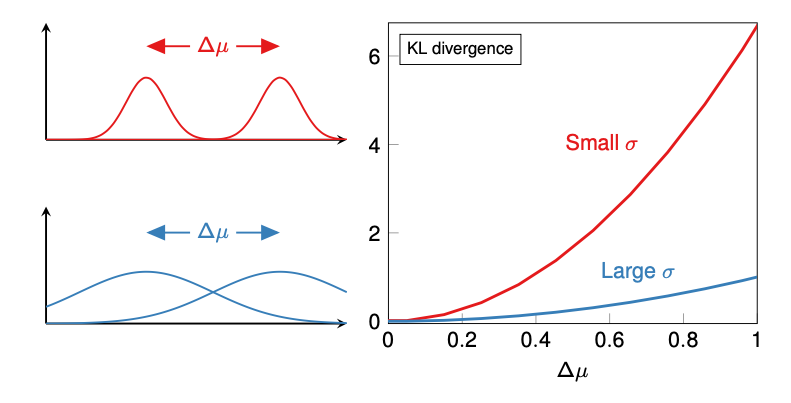
\includegraphics[width=0.9\textwidth]{img/kld_gaussian.png}
    \end{center}
    \begin{itemize}
        \item Consider two Gaussian distributions with \(\sigma_p = \sigma_q\) and let \(\Delta \mu = \mu_p - \mu_q\) represent the difference in their means.
        \item The KL divergence increases more rapidly if two narrow Gaussian distributions (i.e., with smaller variances) are separated further apart in terms of their means.
    \end{itemize}

    So far, we have seen:
    \begin{itemize}
        \item \textbf{Cross-entropy:} Represents the expected code length when using a suboptimal (incorrect) code.
        \item \textbf{KL Divergence:} Measures the difference between two probability distributions and is always non-negative (Gibbs' inequality).
        \item \textbf{Interpretations:}
              \begin{itemize}
                  \item \textit{Compression interpretation:} KL divergence represents the “extra cost” of using an incorrect code.
                  \item \textit{Geometric interpretation:} KL divergence increases as two distributions diverge from each other.
              \end{itemize}
        \item \textbf{Connection to inference:} Minimum code length is mathematically equivalent to maximum likelihood estimation, implying that a good compressor is also a good predictor.
    \end{itemize}

}

\section{Maximum Likelihood Inference}
\defb{Definition: Maximum Likelihood Estimation (MLE)}{Given a dataset \( \mb{x} \) and a family of PDFs \( p(\mb{x}; \theta) \), the maximum likelihood estimate (MLE) of the parameter \( \theta \) is:
    \[
        \theta^*_{\text{MLE}} = \arg \max_{\theta} p(\mb{x}; \theta)
    \]
    MLE is a widely used method in machine learning and data science for estimating model parameters.}


\begin{itemize}
    \item Consider a sample of \( n \) data points \( \mb{x} = \{x_i\}_{i=1}^n \) and a family of probability density functions (PDFs) \( p(\mb{x}; \theta) \) parameterised by \( \theta \).
    \item How do we fit a PDF to $\mb{x}$?


    \item Assuming the data points are independent and identically distributed (i.i.d.), the likelihood of observing \( \mb{x} \) given \( \theta \) is:
          \[
              p(\mb{x}; \theta) = \prod_{i=1}^n p(x_i; \theta)
          \]

    \item It is often convenient to work with the \textbf{log-likelihood function}:
          \[
              L(\theta) = \frac{1}{n} \ln p(\mb{x}; \theta) = \frac{1}{n} \sum_{i=1}^n \ln p(x_i; \theta)
          \]

    \item For large datasets (as \( n \to \infty \)), by the Law of Large Numbers, the log-likelihood converges to the expected value:
          \[
              \lim_{n \to \infty} L(\theta) = \mathbb{E}_p [\ln p(x; \theta)]
          \]
\end{itemize}

\ex{Maximum Likelihood for Gaussian Means}{

    \begin{itemize}
        \item Consider \( n \) i.i.d. data points \( x_1, x_2, \ldots, x_n \) drawn from a Gaussian distribution with unknown mean \( \mu \) and known variance \( \sigma^2 \).

        \item The PDF of each data point under the Gaussian distribution is:
              \[
                  p(x_i; \mu) = \frac{1}{\sqrt{2\pi \sigma^2}} \exp\left(-\frac{(x_i - \mu)^2}{2\sigma^2}\right)
              \]

        \item The log-likelihood function for the mean \( \mu \) is:
              \[
                  L(\mu) = \frac{1}{n} \sum_{i=1}^n \ln p(x_i; \mu) = -\frac{1}{2} \ln(2\pi \sigma^2) - \frac{1}{2n \sigma^2} \sum_{i=1}^n (x_i - \mu)^2
              \]

        \item To find the MLE for \( \mu \), differentiate \( L(\mu) \) with respect to \( \mu \) and set the derivative to zero:
              \[
                  \frac{dL}{d\mu} = \frac{1}{n \sigma^2} \sum_{i=1}^n (x_i - \mu) = 0
              \]

              \begin{center}
                  \begin{tikzpicture}
                      \begin{axis}[
                              domain=-5:5,
                              samples=100,
                              axis x line=middle,
                              axis y line=middle,
                              xlabel={\(\mu\)},
                              ylabel={\(\mathcal{L}\)},
                              ymin=-11, ymax=-3,
                              xmin=-5, xmax=5,
                              xtick={-5,0,5},
                              ytick={-10,-8,-6,-4},
                              width=6cm,
                              height=4cm,
                              y label style={at={(axis description cs:0.05,1.1)}},
                              x label style={at={(axis description cs:1.05,0.1)}}
                          ]
                          % Log-likelihood curve
                          \addplot[blue, thick] {-(x^2 / 2) - 5.5};
                          % Vertical line for MLE
                          \addplot[dashed] coordinates {(0,-11) (0,-3)};
                          % MLE label
                          \node at (axis cs:0,-10.5) [anchor=north east] {\(\mu^*_{\text{MLE}}\)};
                      \end{axis}
                  \end{tikzpicture}
              \end{center}

        \item Solving this equation, we obtain:
              \[
                  \mu^*_{\text{MLE}} = \frac{1}{n} \sum_{i=1}^n x_i
              \]
              Thus, the MLE for the mean \( \mu \) is simply the sample mean.
    \end{itemize}
}

\subsection{A Good Compressor is a Good Predictor}

\begin{itemize}
    \item Suppose we have:
          \begin{itemize}
              \item Data \( X \sim p(x) \)
              \item A compressor that uses code lengths \( \ell(x) \)
          \end{itemize}

    \item This means the compressor has learned some certain implicit probabilities \( q(x) \) by setting:
          \[
              q(x) = \frac{1}{z} 2^{-\ell(x)} \quad \text{where} \quad z = \sum_x 2^{-\ell(x)} \quad \text{ and } \ell(x) = -\log z - \log q(x)
          \]

          \(z\) is known as the Kraft number, where the Kraft inequality is satisfied if \( z \leq 1 \).

    \item \hl{By the Source Coding Theorem (SCT), the optimal code length is:
    \[
        \ell^*(x) = -\log p(x)
    \]}


    \item The expected extra cost incurred by using \( q \) instead of the true distribution \( p \) is:
          \begin{align*}
              \mathbb{E}_p [\ell(x) - \ell^*(x)] & = \mathbb{E}_p\left[ -\log x - \log q(x) + \log p(x)\right] \\
                                                 & = \log \frac{1}{z} + D_{KL}(p \parallel q)
          \end{align*}

          where \(\log \frac{1}{z} \geq 0\) by the Kraft inequality. This extra cost is zero iff:
          \begin{itemize}
              \item Kraft eqaulity is achieved, or the `supermarket budget' is spent
              \item The two distributions are the same, i.e., \( p = q \)
          \end{itemize}

          \[
              L = L^* \Leftrightarrow p = q
          \]

    \item Therefore, an optimal compressor has effectively ``learned" the true data distribution.
\end{itemize}

\intuitb{Summary}{
    \begin{itemize}
        \item Symbol codes compress individual symbols, not blocks. Prefix codes are especially useful due to the Kraft inequality and their tree representation.
        \item \textbf{KL Divergence:} Measures the difference between two probability distributions, always non-negative (Gibbs' inequality).
        \item \textbf{Interpretations:}
              \begin{itemize}
                  \item \textit{Compression interpretation:} KL divergence quantifies the “extra cost” of using an incorrect code.
                  \item \textit{Geometric interpretation:} KL divergence increases as two distributions become more dissimilar.
              \end{itemize}
        \item \textbf{Inference connection:} Minimum code length corresponds to maximum likelihood estimation, i.e. a good compressor is a good predictor.
    \end{itemize}
}

\chapter{Joint Entropy}

\section{Multivariate Distributions}

\subsection{Partitioning the Sample Space}
A random variable \( X \) can be viewed as a partition of the sample space \( \Omega \), where each outcome in \( \Omega \) is associated with a specific value of \( X \). This partitions \( \Omega \) into disjoint subsets corresponding to different values of \( X \).

\begin{marginfigure}
    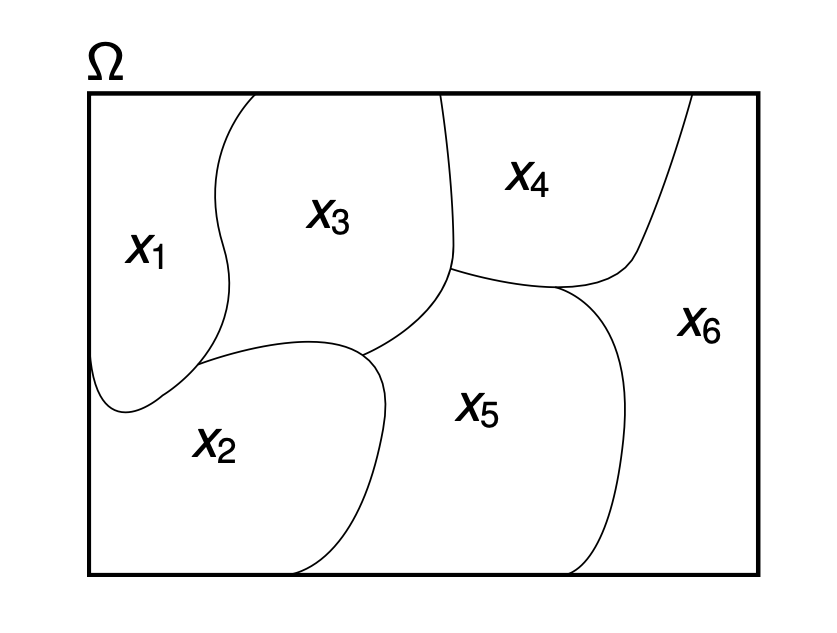
\includegraphics[width=1\textwidth]{img/partition.png}
    \caption{Recall the definition of a random variable as a function from the sample space $\Omega$. We can think of this as a partition of the set $\Omega$.}
\end{marginfigure}


\subsection{Joint Random Variables}
When considering joint random variables \( X \) and \( Y \), these can be thought of as creating different partitions of the same sample space \( \Omega \). The joint probability \( p(X = x, Y = y) \) represents the intersection of the preimages of \( x \) and \( y \), which is the probability of both events happening simultaneously:
\[
    p(X = x, Y = y) = p(\omega \in X^{-1}(x) \cap Y^{-1}(y)).
\]

\begin{center}
    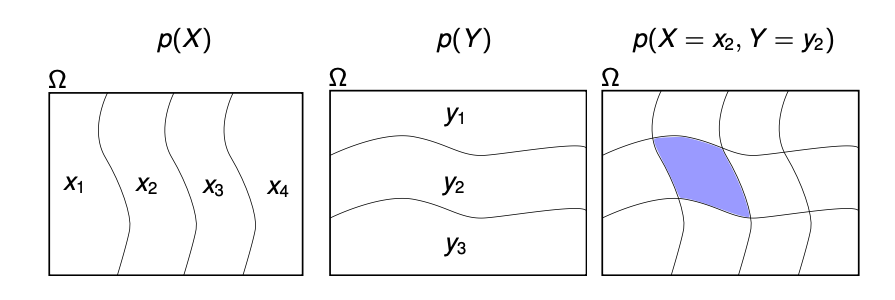
\includegraphics[width=1\textwidth]{img/joint_partition.png}
\end{center}

\ex{Joint Distributions on a Die}{Consider a die, with sample space \( \Omega = \{1, 2, 3, 4, 5, 6\} \). Define two random variables \( X \) and \( Y \):
    \begin{itemize}
        \item \( X \): whether the number rolled is even.
        \item \( Y \): whether the number rolled is greater than 3.
    \end{itemize}


    \begin{center}
        \begin{tabular}{ccc}
            \toprule
            \( \omega \) & \( X(\omega) \) & \( Y(\omega) \) \\
            \midrule
            1            & 0               & 0               \\
            2            & 1               & 0               \\
            3            & 0               & 0               \\
            4            & 1               & 1               \\
            5            & 0               & 1               \\
            6            & 1               & 1               \\
            \bottomrule
        \end{tabular}
    \end{center}

}


\subsection{Marginal and Conditional Probabilities}
The marginal probability \( p(X = x) \) gives the probability of \( X = x \) regardless of \( Y \):
\[
    p(X = x) = \sum_{y \in Y} p(X = x, Y = y).
\]
The conditional probability \( p(X = x | Y = y) \) is the probability of \( X = x \) given that \( Y = y \) has occurred:
\[
    p(X = x | Y = y) = \frac{p(X = x, Y = y)}{p(Y = y)}.
\]

\sn{Conditioning on Impossible Events}{If \( p(Y = y) = 0 \), then \( p(X | Y = y) \) is undefined.}

\subsection{Joint Probability Rules}

Joint probabilities satisfy several fundamental rules:

\begin{itemize}
    \item \textbf{Product Rule:} The probability of the joint occurrence of \( X \) and \( Y \) can be factored as:
          \[
              p(X = x, Y = y) = p(X = x | Y = y) p(Y = y).
          \]

    \item \textbf{Sum Rule:} The marginal probability of \( X = x \) can be derived by summing over all possible values of \( Y \):
          \[
              p(X = x) = \sum_{y \in Y} p(X = x | Y = y) p(Y = y).
          \]

    \item \textbf{Bayes' Theorem:} This rule relates conditional probabilities by switching the conditioning:
          \[
              p(X = x | Y = y) = \frac{p(Y = y | X = x) p(X = x)}{p(Y = y)}.
          \]
    \item The same intuitions apply in continous spaces, with integrals replacing sums.
\end{itemize}

\sn{Warning: Notation Overload}{
    \raggedright
    The symbol \( p \) in expressions like \( p(x) \) and \( p(y) \) technically represents different functions for each variable. For clarity, the precise way to write this would be  \( p_X(X = x) \) or \( p_Y(Y = y) \), though we often simplify to \( p(x) \) when it is unambigious from the context.}

\subsection{Statistical Independence}

\defb{Independent Random Variables}{
    A set of random variables \( \{X_1, X_2, \ldots, X_n\} \) is independent if, for any subset \( \{X_{i_1}, X_{i_2}, \ldots, X_{i_k}\} \),
    \[
        p(X_{i_1}, X_{i_2}, \ldots, X_{i_k}) = p(X_{i_1}) p(X_{i_2}) \cdots p(X_{i_k}).
    \]
    For \( n = 2 \), we denote this as \( X_1 \perp\!\!\!\perp X_2 \), which implies that \( p(X_1 | X_2) = p(X_1) \).
}

We distinguish two types of independence:

\begin{itemize}
    \item \textbf{Marginal Independence:} Two random variables \( X \) and \( Y \) are independent if \( p(X, Y) = p(X) p(Y) \).
    \item \textbf{Conditional Independence:} Given a third variable \( Z \), \( X \) and \( Y \) are conditionally independent if \( p(X, Y | Z) = p(X | Z) p(Y | Z) \), denoted as \( X \perp\!\!\!\perp Y | Z \).
\end{itemize}

\sn{Warning: Conditional Independence}{
    Conditioning on a variable can create or destroy dependence. \bigskip

    \textbf{Example of Creating Independence }
    \begin{itemize}
        \item \( X \) represents whether a person carries an umbrella.
        \item \( Y \) represents whether the ground is wet.
        \item Let \( Z \) represent the weather, sunny or rainy.
    \end{itemize}

    $X$ and $Y$ are dependent because seeing someone with an umbrella makes it more likely that the ground is wet because it's raining. However, if we know the weather, i.e. conditioning on $Z$, then $X$ and $Y$ are independent– given it is raining, knowing the fact of whether a person carries an umbrella no longer provides any additional information about whether the ground is wet.\bigskip

    \textbf{Example of Destroying Independence}
    \begin{itemize}
        \item \( X \) is the outcome of Coin A (heads or tails).
        \item \( Y \) is the outcome of Coin B (heads or tails).
        \item Let \( Z \) whether the coins show the same outcome (heads-heads or tails-tails).
    \end{itemize}
    Say you flip Coin A and Coin B, you know $X$ and $Y$ are independent as the result of one coin flip does not affect the other. However, conditioning on $Z$ (i.e. knowing the coins show the same outcome) destroys this independence. If you know the coins show the same outcome, then the outcome of Coin A tells you the outcome of Coin B, and vice versa.

}


\marginnote{
    \ex{Conditional Independence Example}{
        Let \( f \) and \( g \) be stochastic functions. If \( Y = f(X) \) and \( Z = g(Y) \), then \( X \) and \( Z \) are dependent (\( X \not\perp\!\!\!\perp Z \)) but become conditionally independent given \( Y \), i.e., \( X \perp\!\!\!\perp Z | Y \). \bigskip

        As another example, if \( X \) and \( Y \) are independent fair coin flips (i.e., \( X, Y \sim B(0.5) \)), and \( Z = (X + Y) \mod 2 \), then \( X \) and \( Z \) are independent but become dependent when conditioned on \( Y \).
    }}

\section{Graphical Models}

\defb{Bayesian Network}{
    A \textbf{Bayesian network} is a directed network where each node represents a random variable (RV), and the edges represent a factorisation of the joint probability density function (PDF). Formally, given a set of random variables \( X = \{X_1, X_2, \dots, X_k\} \), the joint distribution is factorised as:
    \[
        p(X) = \prod_{k} p(X_k | \text{pa}(X_k))
    \]
    where \(\text{pa}(X_k)\) denotes the set of parents of \(X_k\). In this representation, the directed edges indicate conditional dependencies among variables.
}

\begin{figure}[h]
    \centering
    % Improved Bayesian Network Diagram
    \begin{tikzpicture}[->, >=stealth, node distance=2cm, thick]
        \node[circle, draw, minimum size=1cm](X) {\(X\)};
        \node[circle, draw, minimum size=1cm, above right of=X](Y) {\(Y\)};
        \node[circle, draw, minimum size=1cm, below right of=X](Z) {\(Z\)};
        \node[circle, draw, minimum size=1cm, below right of=Y](U) {\(U\)};

        \draw[->] (X) -- (Y);
        \draw[->] (X) -- (Z);
        \draw[->] (Y) -- (U);
        \draw[->] (Z) -- (U);
    \end{tikzpicture}
    \caption{Bayesian Network example}
\end{figure}

This network represents the joint probability factorisation:
\[
    p(X, Y, Z, U) = p(X) p(Y|X) p(Z|X) p(U|Y,Z)
\]

\section{Markov Chains and Joint Entropy}

\defb{Markov Chain}{
    A stochastic process \( X_1, X_2, \dots, X_n \) is called a \textbf{Markov chain} if, for all \( t \),
    \[
        p(X_t | X_{t-1}, X_{t-2}, \dots, X_1) = p(X_t | X_{t-1})
    \]
    In other words, each state \( X_t \) depends only on the previous state \( X_{t-1} \), not on earlier states. This is often denoted as \( X_1 \to X_2 \to \dots \to X_n \).
}

% Markov Chain Diagram
\begin{figure}[h]
    \centering
    \begin{tikzpicture}[->, >=stealth, node distance=2cm, thick]
        \node[circle, draw, minimum size=1cm](X1) {\(X_1\)};
        \node[circle, draw, minimum size=1cm, right of=X1](X2) {\(X_2\)};
        \node[circle, draw, minimum size=1cm, right of=X2](X3) {\(X_3\)};
        \node[circle, draw, minimum size=1cm, right of=X3](X4) {\(X_n\)};

        \draw[->] (X1) -- (X2);
        \draw[->] (X2) -- (X3);
        \draw[dashed, ->] (X3) -- (X4);
    \end{tikzpicture}
    \caption{Markov Chain Diagram}
\end{figure}

The above diagram illustrates a simple Markov chain, where each variable depends only on the preceding variable. In writing, we also consider Markov chains of order $p$:

\[p(X_t | X_{t-1}, X_{t-2}, \cdots, X_1) = p(X_t | X_{t-1}, \cdots, X_{t-p})\]

\defb{Joint Entropy}{
    The \textbf{joint entropy} of two random variables \( X \) and \( Y \), with alphabets \( \mathcal{X} \) and \( \mathcal{Y} \), is defined as:
    \[
        H(X, Y) = - \sum_{x \in \mathcal{X}} \sum_{y \in \mathcal{Y}} p(x, y) \log p(x, y)
    \]
    Joint entropy represents the combined uncertainty in predicting both \( X \) and \( Y \) simultaneously. It is symmetric, so \( H(X, Y) = H(Y, X) \).
}

All properties of entropy apply to joint entropy.
\begin{itemize}
    \item Expected value of joint surprisal, $\mathbb{E}_p[-\log p(X, Y)]$, is the joint entropy.
    \item Uncertainty when predicting $X$ and $Y$ jointly.
    \item Minimum code length when encoding $X$ and $Y$ simultaneously.
\end{itemize}

\defb{Conditional Entropy}{
    The \textbf{conditional entropy} of \( X \) given \( Y \), denoted \( H(X|Y) \), represents the uncertainty in \( X \) when \( Y \) is known. It is given by:
    \[
        H(X|Y) = \sum_{y \in \mathcal{Y}} p(y) H(X|Y = y)
    \]
    where
    \[
        H(X|Y = y) = - \sum_{x \in \mathcal{X}} p(x|y) \log p(x|y)
    \]
    Conditional entropy quantifies the remaining uncertainty in \( X \) after observing \( Y \). \bigskip

    Note that $H(X|Y)$ is not defined when $p(Y = y) = 0$ for any $y$. To fix this, we either sum over $y$ such that $p(Y = y) > 0$ or use the limit definition of entropy, where $\frac{0}{0} \log 0 = 0$.
}


Some important properties of conditional entropy for discrete random variables:

\begin{itemize}
    \item \textbf{Non-negativity:} \( H(X|Y) \geq 0 \).

          \textbf{Proof:} Since probabilities \( p(x|y) \leq 1 \), we have \( -\log p(x|y) \geq 0 \). Thus, each term in the summation is non-negative, ensuring \( H(X|Y) \geq 0 \).

    \item \textbf{Upper Bound:} \( H(X|Y) \leq \log |\mathcal{X}| \), where \( |\mathcal{X}| \) is the size of the alphabet of \( X \).

          \textbf{Proof:} This follows similarly to the upper bound on \( H(X) \), using the fact that \( -\log p(x|y) \leq \log |\mathcal{X}| \) for all \( x \).

    \item \textbf{Deterministic Dependency:} \( H(X|Y) = 0 \) if \( X \) is a deterministic function of \( Y \).

          \textbf{Proof:} If \( X \) is completely determined by \( Y \), then \( p(x|y) \) is either \( 1 \) or \( 0 \) for each \( x \) given \( y \), making \( -\log p(x|y) = 0 \) wherever \( p(x|y) = 1 \).

    \item \textbf{Independence:} If \( X \) and \( Y \) are independent, then \( H(X|Y) = H(X) \).

          \textbf{Proof:} Independence implies \( p(x|y) = p(x) \), and so:
          \[
              H(X|Y = y) = - \sum_{x \in \mathcal{X}}p(x|y)\log p(x|y)= - \sum_{x \in \mathcal{X}} p(x) \log p(x) = H(X).
          \]
          Averaging over \( y \) yields \( H(X|Y) = H(X).\)
\end{itemize}

\subsection{Conditional Kullback-Leibler (KL) Divergence}

\defb{Conditional KL Divergence}{
    The \textbf{conditional Kullback-Leibler (KL) divergence} between two conditional probability distributions \( p(X|Y) \) and \( q(X|Y) \) is defined as:
    \[
        D_{\text{KL}}(p(X|Y) \parallel q(X|Y)) = \sum_{y \in \mathcal{Y}} p(y) D_{\text{KL}}(p(X|Y = y) \parallel q(X|Y = y)),
    \]
    where
    \[
        D_{\text{KL}}(p(X|Y = y) \parallel q(X|Y = y)) = \sum_{x \in \mathcal{X}} p(x|y) \log \frac{p(x|y)}{q(x|y)}.
    \]
}

\begin{itemize}
    \item \textbf{Non-negativity:} \( D_{\text{KL}}(p(X|Y) \parallel q(X|Y)) \geq 0 \).

          \textbf{Explanation:}
          The non-negativity follows from the non-negativity of each individual term \( D_{\text{KL}}(p(X|Y = y) \parallel q(X|Y = y)) \), as each conditional KL divergence is non-negative.

    \item \textbf{Zero Value:} \( D_{\text{KL}}(p(X|Y) \parallel q(X|Y)) = 0 \) if and only if \( p(X|Y) = q(X|Y) \) for all \( y \).

          \textbf{Explanation:}
          This holds because each \( D_{\text{KL}}(p(X|Y = y) \parallel q(X|Y = y)) = 0 \) if and only if \( p(x|y) = q(x|y) \) for all \( x \) and \( y \), meaning the two distributions are identical.

    \item \textbf{Additivity:} For independent conditional distributions, \( D_{\text{KL}}(p(X,Y) \parallel q(X,Y)) = D_{\text{KL}}(p(X|Y) \parallel q(X|Y)) + D_{\text{KL}}(p(Y) \parallel q(Y)) \).

          \textbf{Explanation:}
          This property arises because the joint divergence \( D_{\text{KL}}(p(X,Y) \parallel q(X,Y)) \) can be decomposed into divergences over conditional and marginal components when \( p(X|Y) \) and \( q(X|Y) \) are conditionally independent.
\end{itemize}


\ex{Joint and Conditional Entropy Example}{
    Consider random variables \( X \) and \( Y \) with the following probability distribution:

    \begin{center}
        \begin{tabular}{c|cc|c}
            \( p(x, y) \) & \( x = 0 \)       & \( x = 1 \)       & \( p(y) \)        \\
            \hline
            \( y = 0 \)   & \( \frac{1}{8} \) & \( 0 \)           & \( \frac{1}{8} \) \\
            \( y = 1 \)   & \( \frac{1}{8} \) & \( \frac{1}{4} \) & \( \frac{3}{8} \) \\
            \( y = 2 \)   & \( \frac{1}{4} \) & \( \frac{1}{4} \) & \( \frac{1}{2} \) \\
            \hline
            \( p(x) \)    & \( \frac{1}{2} \) & \( \frac{1}{2} \) &                   \\
        \end{tabular}
    \end{center}

    Calculating the entropies for this distribution:

    \begin{itemize}
        \item \( H(X) = 1 \) bit
        \item \( H(Y) = 1.41 \) bits
        \item \( H(X|Y) = 0.84 \) bits
        \item \( H(Y|X) = 1.25 \) bits
        \item \( H(X, Y) = 2.25 \) bits
    \end{itemize}

    This example illustrates how joint and conditional entropies quantify the combined and remaining uncertainties within a pair of random variables.
}

\subsection{Entropy Chain Rule}

\thm{Entropy Chain Rule}{
    For two random variables \( X \) and \( Y \), the entropy chain rule states:
    \[
        H(X, Y) = H(X | Y) + H(Y)
    \]
    This is a foundational property in information theory, allowing the joint entropy \( H(X, Y) \) to be decomposed into the sum of the conditional entropy \( H(X | Y) \) and the marginal entropy \( H(Y) \).


    \paragraph{Proof:}
    Starting with the definition of joint entropy:
    \[
        H(X, Y) = - \sum_{x, y} p(x, y) \log p(x, y)
    \]

    we can rewrite \( p(x, y) \) in terms of the conditional and marginal distributions:
    \[
        = - \sum_{x, y} p(x | y) p(y) \log (p(x | y) p(y))
    \]

    Expanding the logarithm gives:
    \[
        = - \sum_{x, y} p(x | y) p(y) \left( \log p(x | y) + \log p(y) \right)
    \]

    Now we distribute \( p(x | y) p(y) \) across the sum:
    \[
        = - \sum_{x, y} p(x | y) p(y) \log p(x | y) - \sum_{x, y} p(x | y) p(y) \log p(y)
    \]

    The first term simplifies to the conditional entropy \( H(X | Y) \):
    \[
        = H(X | Y) - \sum_{y} p(y) \log p(y) \underbrace{\sum_{x} p(x | y)}_{= 1}
    \]

    Since \( \sum_{x} p(x | y) = 1 \) for each \( y \), the second term becomes:
    \[
        = H(X | Y) - \sum_{y} p(y) \log p(y) \cancel{\underbrace{\sum_{x} p(x | y)}_{1}}
    \]

    This simplifies further to:
    \[
        H(X,Y) = H(X | Y) + H(Y)
    \]
    which proves the chain rule.
}

\subsection{Invariance of Entropy under Isomorphisms}


\defb{Isomorphisms of RVs}{
    Two random variables \( X \) and \( Y \) are said to be \textbf{isomorphic} if there exists a bijective (one-to-one and onto) function \( f \) such that:
    \[
        X = f(Y) \quad \text{and} \quad Y = f^{-1}(X)
    \]
    This implies that \( X \) and \( Y \) can be perfectly mapped to each other without any loss of information. Therefore, the uncertainty (entropy) of \( X \) is exactly the same as that of \( Y \).
}

\begin{marginfigure}
    \centering
    \resizebox{1\linewidth}{!}{ % Adjust 0.8\linewidth to scale as desired
        \begin{tikzpicture}[ele/.style={fill=black,circle,minimum width=.8pt,inner sep=1pt, scale=0.5},every fit/.style={ellipse,draw,inner sep=-2pt}]
            \node[ele,label=left:$a$] (a1) at (0,4) {};
            \node[ele,label=left:$b$] (a2) at (0,3) {};
            \node[ele,label=left:$c$] (a3) at (0,2) {};
            \node[ele,label=left:$d$] (a4) at (0,1) {};

            \node[ele,label=right:$1$] (b1) at (4,4) {};
            \node[ele,label=right:$2$] (b2) at (4,3) {};
            \node[ele,label=right:$3$] (b3) at (4,2) {};
            \node[ele,label=right:$4$] (b4) at (4,1) {};

            \node[draw,fit= (a1) (a2) (a3) (a4),minimum width=2cm] {} ;
            \node[draw,fit= (b1) (b2) (b3) (b4),minimum width=2cm] {} ;
            \draw[->,thick,shorten <=2pt,shorten >=2pt] (a1) -- (b4);
            \draw[->,thick,shorten <=2pt,shorten >=2pt] (a2) -- (b2);
            \draw[->,thick,shorten <=2pt,shorten >=2pt] (a3) -- (b1);
            \draw[->,thick,shorten <=2pt,shorten >=2pt] (a4) -- (b3);
        \end{tikzpicture}
    }
    \caption{Visualisation of a bijective function between two sets of random variables.}
\end{marginfigure}

\thm{Invariance of Entropy}{
    Entropy is invariant under isomorphisms of discrete random variables. Specifically, if two random variables \( X \) and \( Y \) are isomorphic, then \( H(X) = H(Y) \).


    \paragraph{Proof:}
    We can demonstrate this by applying the entropy chain rule in both directions:
    \[
        H(X, Y) = H(X) + H(Y | X) = H(Y) + H(X | Y)
    \]

    Since \( X = f(Y) \), knowing \( Y \) completely determines \( X \), meaning \( H(X | Y) = 0 \). Similarly, \( Y = f^{-1}(X) \) implies \( H(Y | X) = 0 \).

    Thus, we have:
    \[
        H(X) = H(Y)
    \]
    which confirms that the entropy of \( X \) is equal to the entropy of \( Y \) when they are isomorphic.
}

\section{Stochastic Processes}

Previously, we covered the case of two RVs, $X$ and $Y$, but can extend this to $n$ joint RVs with stochastic processes.

\defb{Stochastic Process}{
A \textbf{stochastic process} is a collection of random variables indexed by time (or another ordering parameter). Formally, a stochastic process is represented as \( \{X_i\}_{i \in T} \), where \( T \) is the index set, and each \( X_i \) is a random variable. Here, we will consider semi-infinite processes \( \{X_1, X_2, \dots, X_n\} \).
}

\defb{Stationary Stochastic Process}{
    A stochastic process is \textbf{stationary} if its statistical properties are invariant to shifts in time. For a stationary process, the joint distribution of any subset of variables is the same, regardless of the starting point. \bigskip

    Formally, a stochastic process has, for all \( t \) and \( s \):
    \[
        p(X_1, X_2, \dots, X_t) = p(X_{1+s}, X_{2+s}, \dots, X_{t+s})
    \]
    In essence, time shifts do not alter the distribution.
}

\subsection{Entropy Rate and Innovation}

\defb{Entropy Rate}{
    Refers to how quickly \( H(X_1, X_2, \dots, X_n) \) grows as \( n \) becomes large. \bigskip

    The \textbf{entropy rate} of a stochastic process measures the asymptotic growth rate of the joint entropy \( H(X_1, X_2, \dots, X_n) \) as \( n \) becomes large. For a stationary process \( \{X_i\} \), the entropy rate \( h(X) \) is defined as:
    \[
        h_1(X) = \lim_{n \to \infty} \frac{1}{n} H(X_1, X_2, \dots, X_n)
    \]
}

\defb{Innovation}{
    Refers to how much new information is introduced at time $n$. \bigskip

    \textbf{Innovation} quantifies the amount of new information introduced by each new observation in a stochastic process. It is defined as the conditional entropy of the next observation given all past observations:
    \[
        h_2(X) = \lim_{n \to \infty} H(X_n | X_1, X_2, \dots, X_{n-1})
    \]
}

\thm{Entropy Rate Theorem}{
    For a stationary stochastic process, the entropy rate and the innovation rate are equal:
    \[
        h(X) = \lim_{n \to \infty} \frac{1}{n} H(X_1, X_2, \dots, X_n) = \lim_{n \to \infty} H(X_n | X_1, X_2, \dots, X_{n-1})
    \]
    This result provides a way to measure the information growth in a stationary process by either the average entropy per observation or the amount of new information introduced at each step.
}
\newpage
\marginnote[8.5pt]{
    \thm{Cesaro Mean}{
        \raggedright
        The Cesaro Mean Theorem states, if $a_n \to a$, and $b_n = \frac{1}{n} \sum_{i=1}^n a_i$, then $b_n \to a$. \label{thm:cesaro} \bigskip

        Since $a_n \to a$, there exists a number $N(\epsilon)$ such that for all $n \geq N(\epsilon)$, $|a_n - a| < \epsilon$. Hence,
        \begin{align*}
            \left| b_n - a \right| & = \left| \frac{1}{n} \sum_{i=1}^{n} (a_i - a) \right|                       \\
                                   & \leq \frac{1}{n} \sum_{i=1}^{n} \left| a_i - a \right|                      \\
                                   & \leq \frac{1}{n} \sum_{i=1}^{N(\epsilon)} \left| a_i - a \right| +          \\ &  \quad \frac{n - N(\epsilon)}{n} \epsilon  \\
                                   & \leq \frac{1}{n} \sum_{i=1}^{N(\epsilon)} \left| a_i - a \right| + \epsilon
        \end{align*}

        For all \( n \geq N(\epsilon) \). Since the first term goes to 0 as \( n \to \infty \), we can make \( |b_n - a| \leq 2\epsilon \) by taking \( n \) large enough. Hence \( b_n \to a \) as \( n \to \infty \). \(\qed\)



    }
}
\extrab{Proof of the Entropy Rate Theorem}{

    See Cover \& Thomas (1991) Theorem 4.2.1. We want to show
    \[
        h(X) = \underbrace{\lim_{n \to \infty} \frac{1}{n} H(X_1, X_2, \dots, X_n)}_{h_1(X)} = \underbrace{\lim_{n \to \infty} H(X_n | X_1, X_2, \dots, X_{n-1})}_{h_2(X)}
    \]



    We first show that the $h_2(X)$ limit exists, that the sequence of conditional entropies is a decreasing sequence. We have:
    \begin{align}
        H(X_{n+1}| X_1, X_2, \dots, X_n) & \leq H(X_{n+1} | X_n, X_{n-1}, \dots, X_2)                                    \\&= H(X_n| X_{n-1}, \dots, X_2, X_1) \label{eq:equality_stationarity} \\
        % \\
        % \Rightarrow h_2(X)               & \leq H(X_n| X_{n-1}, \dots, X_2, X_1)                                         \\
        \Rightarrow h_2(X)               & = \lim_{n \to \infty}  H(X_n| X_{n-1}, \dots, X_2, X_1) \label{eq:innovation}
    \end{align}

    where the inequality follows from the fact that conditioning on more variables reduces entropy. The first equality in \ref{eq:equality_stationarity} follows from the stationarity of the process (Markov). For \ref{eq:innovation}, since $H(X_n| X_{n-1}, \dots, X_2, X_1)$ is a decreasing sequence of nonnegative numbers, it has a limit which is the innovation rate. \bigskip



    By the chain rule,
    \[
        H(X_1, X_2) = H(X_1 | X_2) + H(X_2)
    \]
    We can then extend this to \( H(X_1, X_2, X_3) \) as:
    \begin{align*}
        H(X_1, X_2, X_3) & = H(X_1 | X_2, X_3) + H(X_2, X_3)         \\
                         & = H(X_1 | X_2, X_3) +  H(X_2 | X_3) + X_3
    \end{align*}

    The general formula is:

    \begin{equation}
        H(X_1, X_2, \dots X_n) = \sum_{i=1}^n H(X_i | X_{i-1}, X_{i-2}, \dots, X_1)
    \end{equation}
    i.e,the entropy rate is the time average of the conditional entropies. From the Cesaro Mean Theorem, we have
    \begin{align*}
        \frac{1}{n}H(X_1, X_2, \dots X_n)                     & = \frac{1}{n} \sum_{i=1}^n H(X_i | X_{i-1}, X_{i-2}, \dots, X_1)                     \\
        \lim_{n \to \infty} \frac{1}{n}H(X_1, X_2, \dots X_n) & = \lim_{n \to \infty} \frac{1}{n} \sum_{i=1}^n H(X_i | X_{i-1}, X_{i-2}, \dots, X_1) \\
                                                              & = \lim_{n \to \infty} H(X_n | X_{n-1}, \dots, X_2, X_1)
        = h_2(X)\end{align*}


    The running average has a limit, equal to the innovation rate $h_2(X)$ of the terms. This proves the equivalence of $h_1(X)$ and $h_2(X)$, and the entropy rate theorem.

    \[
        h_1(x) = \lim_{n \to \infty} \frac{1}{n}H(X_1, X_2, \dots, X_n) = \lim_{n \to \infty} H(X_n| X_{n-1}, \dots, X_2, X_1) = h_2(X)
    \] \hfill \(\blacksquare\)

}
\newpage
\section{Stochastic Processes}
\[
    H(X_{n+1} | X_1, \dots, X_n) \leq H(X_n | X_1, \dots, X_{n-1})
\]
\begin{itemize}
    \item When conditioning on no prior information (i.e., \( t = 0 \)), we have the full entropy \( H(X_n) \).
    \item As we condition on more previous observations, the conditional entropy decreases.
    \item Intuitively, $X$ is a time series, and $H(X_n | X_1, \dots, X_{n-1})$ is the performance of a predictor with $t$ timesteps of `memory'. Without memory $(t=0)$, we get usual entropy $H(X_n)$, with no memory of the past.
    \item Including more memory decreases the conditional entropy, as the predictor can use past observations to improve predictions. Eventually, the predictor reaches the entropy rate, where no further improvement is possible.
    \item If this happens at some finite $t = p$, the process is said to have a Markov order of $p$.
\end{itemize}

\begin{marginfigure}
    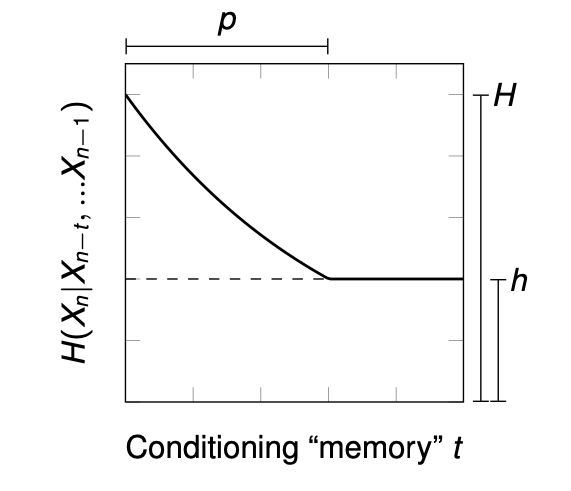
\includegraphics[width=\linewidth]{img/conditioning.png}
    \caption{In this diagram, we see that as the conditioning memory \( t \) increases, the conditional entropy \( H(X_n | X_{n-t}, \dots, X_{n-1}) \) decreases, eventually reaching the entropy rate \( h(X) \).}
\end{marginfigure}

\egb{Coin in a Box}{
    \textbf{Question:} What is the entropy rate of the following process?

    \begin{itemize}
        \item At \( t = 0 \), we flip a fair coin and place it in a box.
        \item At each subsequent time step \( t \), we shake the box, so the coin changes sides with probability \( p \).
    \end{itemize}

    \tcblower
    \textbf{Answer:} The entropy rate of this process as \( n \to \infty \) is given by:
    \begin{align*}
        \lim_{n \to \infty} \frac{1}{n} H(X_1, X_2, \dots, X_n) & = \lim_{n \to \infty} H(X_n | X_1, X_2, \dots, X_{n-1}) \\
                                                                & = H(X_{t+1} | X_t)                                      \\
                                                                & = H_2(p)
    \end{align*}
    where \( H_2(p) \) denotes the entropy of a biased coin with parameter \( p \).
}

\begin{itemize}
    \item The entropy rate measures the average amount of new information introduced by each step in a process.
    \item Useful for applications like compressing sequential data (e.g., language).
    \item "Stream codes," such as the Lempel-Ziv algorithm (used in compression formats like ZIP), are practical applications of entropy rates in stochastic processes.
\end{itemize}

\section{Mutual Information}

\defb{Mutual Information}{
    The mutual information between two random variables \( X \) and \( Y \) is defined as:
    \[
        I(X;Y) := \sum_{x,y \in \mathcal{X} \times \mathcal{Y}} p(x, y) \log \frac{p(x, y)}{p(x)p(y)}.
    \]
    This quantity, often denoted \( I(X; Y) \), measures the reduction in uncertainty of \( X \) given knowledge of \( Y \) (or vice versa).
    \begin{itemize}
        \item Mutual information is symmetric: \( I(X; Y) = I(Y; X) \).
        \item To separate the arguments in mutual information (MI), we use a semicolon (;) rather than a comma (,) for separating RVs, e.g., \( I(X; Y) \).
        \item In physics and some other fields, the arguments in mutual information are separated by a colon (:), so \( I(X: Y) \) may also be used.
    \end{itemize}
}



Mutual information can also be expressed as a difference in entropies:
\[
    I(X; Y) = H(X) + H(Y) - H(X, Y).
\]
Using the entropy chain rule, this can be further decomposed as:
\[
    I(X; Y) = \underbrace{H(X)}_{\text{Uncertainty about } X}- \underbrace{H(X | Y)}_{\text{uncertainty about } X \text{ given } Y}
\]
where \( I(X; Y) \) represents the average reduction in uncertainty about \( X \) given \( Y \).
\begin{itemize}
    \item Mutual information cannot exceed the minimum entropy of the two variables: \( I(X; Y) \leq \min \{ H(X), H(Y) \} \).
\end{itemize}


\subsection{Mutual Information as KL Divergence}
Mutual information can be interpreted as the Kullback-Leibler (KL) divergence between the joint probability distribution \( p(X, Y) \) and the product of the marginal distributions \( p(X)p(Y) \):
\begin{equation}
    I(X; Y) = D_{KL}(p(X, Y) \parallel p(X)p(Y)). \label{eq:mi_kl}
\end{equation}

\marginnote[-70pt]{
    Equation \ref{eq:mi_kl} implies two very important key properties:
    \begin{itemize}
        \item \textbf{Non-negativity}: Since KL divergence is always non-negative, mutual information \( I(X; Y) \geq 0 \).
        \item \textbf{Zero MI for Independence}: Mutual information is zero if and only if \( X \) and \( Y \) are independent, i.e., \( p(X, Y) = p(X)p(Y) \).

              This is because the KL divergence between two identical distributions is zero.


              $D_{KL}(p(X, Y) \parallel p(X)p(Y)) = 0 \Leftrightarrow p(X, Y) = p(X)p(Y)$.
    \end{itemize}}


\thm{Information Doesn’t Hurt}{
    For any two random variables \( X \) and \( Y \), conditioning on \( Y \) reduces the entropy of \( X \):
    \[
        H(X | Y) \leq H(X).
    \]


    \paragraph{Proof: }
    This result follows from the definition of mutual information:
    \[
        H(X) - H(X | Y) = I(X; Y) \geq 0,
    \]
    since mutual information \( I(X; Y) \) is always non-negative. Hence,
    \[
        H(X | Y) \leq H(X).
    \]
}

\begin{itemize}
    \item For continuous random variables, this inequality holds even though \( H(X) \) and \( H(X | Y) \) can individually be negative.
    \item In general, the conditional entropy \( H(X | Y = y) \) can sometimes exceed \( H(X) \), depending on the specific values of \( Y = y \).
\end{itemize}

\subsection{Conditional Mutual Information}
\marginnote{Since conditional mutual information can be viewed as a KL divergence, it has the following properties:
    \begin{itemize}
        \item \textbf{Non-negativity}: \( I(X; Y | Z) \geq 0 \).
        \item \textbf{Zero Condition}: \( I(X; Y | Z) = 0 \) if and only if \( X \) and \( Y \) are conditionally independent given \( Z \) (denoted \( X \perp\!\!\!\perp Y | Z \)).
    \end{itemize}}
\defb{Conditional Mutual Information}{
    The conditional mutual information (CMI) between random variables \( X \) and \( Y \) given \( Z \) is defined as:
    \[
        I(X; Y | Z) := \sum_{x, y, z \in \mathcal{X} \times \mathcal{Y} \times \mathcal{Z}} p(x, y, z) \log \frac{p(x, y | z)}{p(x | z) p(y | z)}.
    \]
    Conditional mutual information quantifies the amount of information shared between \( X \) and \( Y \) when conditioned on a third variable \( Z \).

    \begin{itemize}
        \item We can rewrite the CMI in terms of conditional entropies:
              \begin{align*}
                  I(X; Y | Z) & = H(X | Z) + H(Y | Z) - H(X, Y | Z) \\
                              & = H(X | Z) - H(X | Y, Z)
              \end{align*}

        \item CMI is a KL divergence:
              \[
                  I(X; Y | Z) = D_{\text{KL}}(p(X, Y | Z) \parallel p(X | Z)p(Y | Z))
              \]
    \end{itemize}

}





\section{Chain Rule for Mutual Information}

\thm{Mutual Information Chain Rule}{
    The chain rule for mutual information states that for any three random variables \( X \), \( Y \), and \( Z \):
    \[
        I(X, Y; Z) = I(X; Z) + I(Y; Z | X).
    \]

    That is, the mutual information between \( X \) and \( Y \) given \( Z \) can be decomposed into the mutual information between \( X \) and \( Z \) and the conditional mutual information between \( Y \) and \( Z \) given \( X \).

    \paragraph{Proof:}
    The proof of the chain rule follows from the properties of joint and conditional entropy:
    \[
        I(X, Y; Z) = H(X, Y) - H(X, Y | Z).
    \]
    Applying the chain rule for entropy, we can expand \( H(X, Y) \) and \( H(X, Y | Z) \). We rearrange and simplify:
    \begin{align}
        I(X, Y; Z) & = H(X, Y) - H(X, Y | Z)                                                                      \\
                   & = H(Y | X) + H(X) - \left( H(Y | X, Z) + H(X | Z) \right) \label{eq:mi_entropy_chain_rule}   \\
                   & = \underbrace{H(X) - H(X | Z)}_{I(X; Z)} + \underbrace{H(Y | X) - H(Y | X, Z)}_{I(Y; Z | X)} \\
                   & = I(X; Z) + I(Y; Z | X).
    \end{align}

    where the second equality follows from the entropy chain rule (see Equation~\ref{eq:mi_entropy_chain_rule}).

}


\pagebreak
\section{Mutual Information Invariance}
\marginnote[11pt]{\thm{Data Processing Inequality (DPI)}{
        If \( X \), \( Y \), and \( Z \) form a Markov chain \( X \to Y \to Z \), then:
        \[
            I(X; Z) \leq I(X; Y).
        \]
        \paragraph{Proof:}
        \begin{itemize}
            \item Applying the MI chain rule in both directions:
                  \begin{align*}
                       & I(X; Y, Z)              \\
                       & = I(X; Z) + I(X; Y | Z) \\
                       & = I(X; Y) + I(X; Z | Y)
                  \end{align*}

            \item By the definition of a Markov chain, \( X \perp\!\!\!\perp Z | Y \), and thus \( I(X; Z | Y) = 0 \).

            \item By the non-negativity of conditional mutual information (CMI), \( I(X; Y | Z) \geq 0 \). Thus,
                  \[
                      I(X; Z) \leq I(X; Y).
                  \]
        \end{itemize}
    }}

\marginnote{
    \sn{Note on Continuous Variables}{
        This invariance property also holds for continuous random variables, even though entropy terms such as \( H(X) \) and \( H(X | Y) \) may not themselves be invariant.
    }
}
\thm{Invariance of Mutual Information}{
    Mutual information \( I(X; Y) \) is invariant under bijective (one-to-one and onto) transformations of \( X \) or \( Y \).

    \paragraph{Proof:}

    Let \( V = f(Y) \), where \( f \) is a bijective function. This gives a new variable \( V \) that preserves all information in \( Y \). Since \( X \), \( Y \), and \( V \) form a Markov chain \( X \to Y \to V \), we can apply the \textbf{Data Processing Inequality (DPI)}:
    \[
        I(X; V) \leq I(X; Y).
    \]

    Similarly, because \( f \) is bijective, there exists an inverse \( f^{-1} \) such that \( Y = f^{-1}(V) \). This reverses the dependency chain, making \( X \to V \to Y \) a valid Markov chain, and by DPI, we have:
    \[
        I(X; Y) \leq I(X; V).
    \]

    Combining these two inequalities, we obtain:
    \[
        I(X; Y) = I(X; V),
    \]
    demonstrating that mutual information is preserved under bijective transformations of either variable.
}


\subsection{Connections with Set Theory}

\marginnote{\begin{align*}
        H(X)     & \leftrightarrow \mu                \\
        H(X, Y)  & \leftrightarrow \mu(A \cup B)      \\
        H(X | Y) & \leftrightarrow \mu(A \setminus B) \\
        I(X; Y)  & \leftrightarrow \mu(A \cap B)
    \end{align*}
}

The relationship between entropy and mutual information can be visualised with a Venn diagram:
\begin{itemize}
    \item \( H(X) \) and \( H(Y) \) represent the total uncertainties of \( X \) and \( Y \), respectively.
    \item \( I(X; Y) \) represents the shared information or overlap between \( X \) and \( Y \), i.e., the reduction in uncertainty about one variable given the other.
    \item \( H(X | Y) \) and \( H(Y | X) \) represent the remaining uncertainties in \( X \) and \( Y \) after conditioning on each other.
\end{itemize}


\begin{figure}[h]
    \centering
    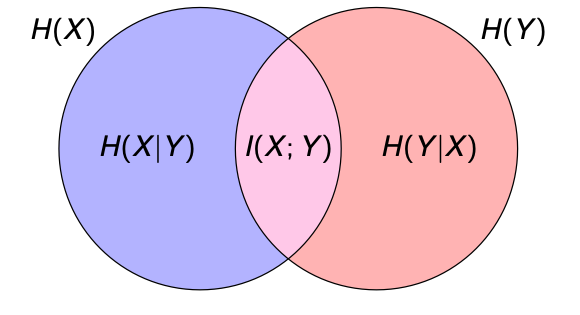
\includegraphics[width=0.6\linewidth]{img/hi_venn.png}
    \caption{Venn diagram illustrating the relationship between entropy and mutual information.}
\end{figure}






In set-theoretic terms, we can extend mutual information to more than two variables. The co-information \( I(X; Y; Z) \) is defined as:
\[
    I(X; Y; Z) = H(X, Y, Z) - H(X, Y) - H(Y, Z) - H(X, Z) + H(X) + H(Y) + H(Z).
\]

\begin{itemize}
    \item Note that co-information \( I(X; Y; Z) \) can be negative depending on how the variables interact. Information, is in fact, a signed measure (an extension of a standard measure in measure theory, which can assign both positive and negative values to sets).
\end{itemize}

\begin{figure}[t]
    \centering
    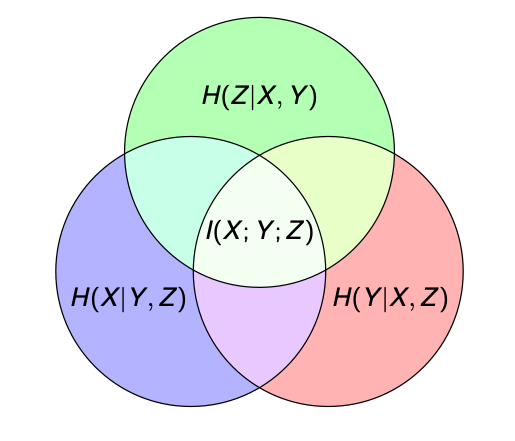
\includegraphics[width=0.6\linewidth]{img/hi_venn_co.png}
    \caption{Venn diagram illustrating three variables and their mutual information}
\end{figure}

\marginnote[-70pt]{
    \refsb{Related Reading}{
        Down \& Mediano. A Logarithmic Decomposition for Information. ISIT 2023.
    }
}

\section{Mutual Information in Gaussian Distributions}

\defb{Mutual Information for Joint Gaussian Variables}{
For two jointly Gaussian random variables \( X \) and \( Y \) with covariance matrix
\[
    \Sigma =
    \begin{pmatrix}
        \sigma_{xx} & \sigma_{xy} \\
        \sigma_{yx} & \sigma_{yy}
    \end{pmatrix} \quad \text{and}\quad  |\Sigma| = \sigma_{xx} \sigma_{yy} - \sigma_{xy}^2
\]
where \( \sigma_{xx} = \mathrm{var}(X) \), \( \sigma_{yy} = \mathrm{var}(Y) \), \(\sigma^2_{y|x} = \sigma^2+y - \sigma^2_{xy}\sigma_x^{-2} \) the mutual information \( I(X; Y) \) can be derived using entropy calculations.
}

See Definition \ref{def:gaussian_entropy} for the entropy of a Gaussian variable. The mutual information \( I(X; Y) \) between \( X \) and \( Y \) can be computed as:
\begin{align*}
    I(X; Y) & = H(X) + H(Y) - H(X, Y)                                                                                            \\
            & = \frac{1}{2} \ln (2 \pi e \sigma_{xx}) + \frac{1}{2} \ln (2 \pi e \sigma_{yy}) - \frac{1}{2} \ln |2 \pi e \Sigma| \\
            & = -\frac{1}{2} \ln \left( \frac{\sigma_{xx} \sigma_{yy} - \sigma_{xy}^2}{\sigma_{xx} \sigma_{yy}} \right)          \\
            & = -\frac{1}{2} \ln \left( 1 - \frac{\sigma_{xy}^2}{\sigma_{xx} \sigma_{yy}} \right)                                \\
            & = -\frac{1}{2} \ln (1 - \rho_{xy}^2) \quad \text{(Correlation)}                                                          \\
            & = \frac{1}{2} \ln \left( \frac{\sigma_{yy}}{\sigma_{y|x}} \right)\quad  \text{(Explained variance)}
\end{align*}
where \( \rho_{xy} = \frac{\sigma_{xy}}{\sqrt{\sigma_{xx} \sigma_{yy}}} \) is the correlation coefficient between \( X \) and \( Y \).

\pagebreak
\subsubsection{Interpretation}
For jointly Gaussian variables, mutual information \( I(X; Y) \) depends only on the correlation \( \rho_{xy} \). As \( \rho_{xy} \) approaches 1 (perfect correlation), \( I(X; Y) \) increases, indicating high shared information. When \( \rho_{xy} = 0 \) (independence), \( I(X; Y) = 0 \), indicating no shared information. This is visualised in Figure \ref{fig:ml_gauss}.



\begin{figure}[h]
    \centering
    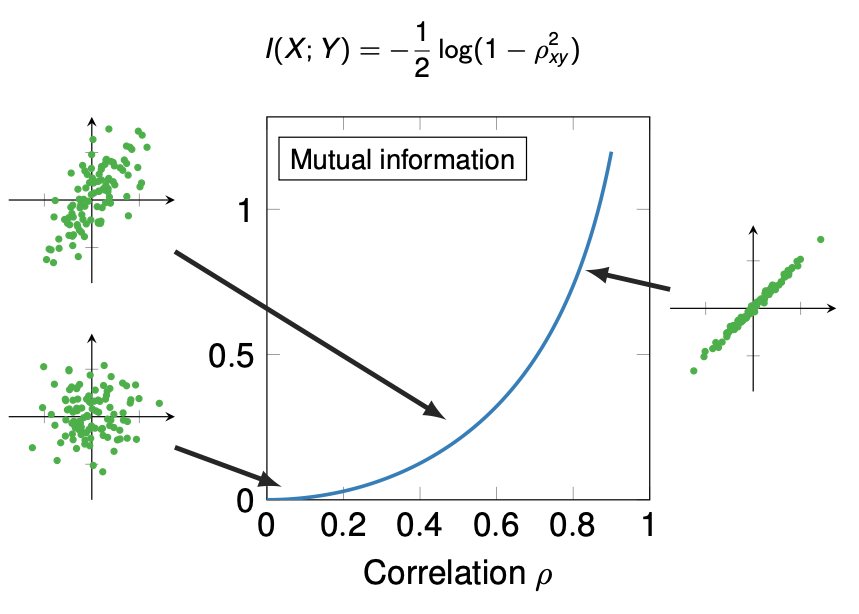
\includegraphics[width=1\linewidth]{img/ml_gauss.png}
    \caption{Maximum Likelihood Estimation for a Gaussian Distribution}
    \label{fig:ml_gauss}
\end{figure}



\begin{itemize}
    \item \textbf{Zero Correlation Does Not Imply Independence}: Two variables can have zero correlation (i.e., no linear relationship) but still be interdependent. See Figure \ref{fig:uncorrelated_interdependent} for examples. Even if \( \rho = 0 \), \( I(X; Y) \) may be greater than zero if there is a dependency that is not linear. 
    \item \textbf{MI as a General Dependency Measure}: Mutual information (MI) is a generalised measure of statistical dependence that captures any form of dependency between two variables, including non-linear relationships (unlike correlation, which only captures linear relationships).
\end{itemize}


\begin{figure}[h]
    \centering
    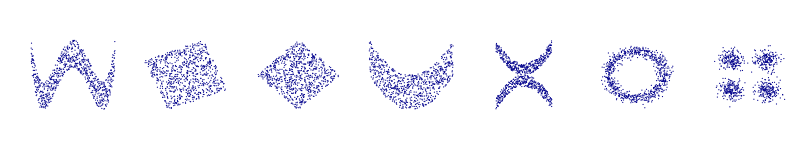
\includegraphics[width=1\textwidth]{img/uncorrelated_interdependent.png}
    \caption{Examples of Distributions where variables are uncorrelated but interdependent}
    \label{fig:uncorrelated_interdependent}
\end{figure}

\section{Mutual Information and Prediction}

In a supervised learning context, mutual information can be used to measure the information about the target variable \( Y \) that is contained in the predictor variable \( X \). Given a dataset with samples \( \{(x_i, y_i)\} \), we can think of mutual information as an upper bound on the predictive performance.

\subsubsection{Applying Gibbs' Inequality}
Consider a parametric family of models \( \mathcal{Q} = \{ q_\theta(y | x) : \theta \in \Theta \} \), where \( q_\theta(y | x) \) is a predictive model (e.g., a neural network or linear model). By applying Gibbs' inequality:
\[
\mathbb{E}_p \left[ \log \frac{p(y | x)}{q_\theta(y | x)} \right] \geq 0,
\]
we obtain:
\begin{align*}
    I(X; Y) & = H(Y) - H(Y | X) \\
            & = H(Y) + \mathbb{E}_{p(x, y)} [\log p(y | x)] \\
            & \geq H(Y) + \underbrace{\mathbb{E}_{p(x, y)} [\log q_\theta(y | x)]}_{\text{Log-likelihood of the predictor on the data}}
\end{align*}

\subsubsection{Implication for Predictive Models}
This shows that if $p(y|x) \in \mathcal{Q}$, 
\[
I(X; Y) \geq \max_{\theta \in \Theta} \left\{ H(Y) + \mathbb{E}_{p(x, y)} [\log q_\theta(y | x)] \right\},
\]
which means that \textbf{mutual information serves as an upper bound on the expected log-likelihood (performance) of the best predictor in the model family} \( \mathcal{Q} \). Therefore, \( I(X; Y) \) represents the maximum achievable performance of any model within this family, making it a useful theoretical benchmark for prediction tasks.

\sn{Summary of Key Points}{
\begin{itemize}
    \item We defined multivariate information quantities, including joint and conditional entropy.
    \item We introduced graphical models and Markov chains as ways to model dependencies between random variables.
    \item \textbf{Mutual Information (MI)} is:
        \begin{itemize}
            \item A generalised measure of statistical interdependence.
            \item Equivalent to explained variance in Gaussian distributions.
            \item An upper bound for the best achievable performance in prediction tasks.
            \item Which is, equivalently, lower-bounded by any regression model. (Any achievable performance from a regression model in terms of predicting $Y$ from $X$ will be less than or equal to the total possible information given by $I(X;Y)$).
        \end{itemize}
    \item Entropy and mutual information both satisfy useful chain rules, which simplify calculations and provide insight into dependency structures.
\end{itemize}
}

\chapter{Channel Coding}

\section{Noisy Channels}

\subsection{The Big Picture}
\begin{itemize}
    \item Previously, we explored source codes under ideal, noiseless conditions.
    \item However, this assumption is often unrealistic in practical communication settings.
    \item This lecture introduces the concept of \textbf{noisy channels}, where communication occurs in the presence of noise, affecting both transmission and reception.
\end{itemize}

\subsection{Discrete Memoryless Channel (DMC)}
\defb{Discrete Memoryless Channel}{
    A \textbf{discrete memoryless channel (DMC)} consists of:
    \begin{itemize}
        \item \textbf{Input alphabet} \( X \)
        \item \textbf{Output alphabet} \( Y \)
        \item \textbf{Conditional probability distribution} \( p(y|x) \), which represents the probability of receiving output \( y \) given input \( x \).
    \end{itemize}
    For longer messages, we consider the \textbf{extended channel} \( p(y^n|x^n) = \prod_{i=1}^{n} p(y_i|x_i) \), where \( n \) independent transmissions occur in parallel.
}

\subsection{Binary Symmetric Channel (BSC)}
\begin{marginfigure}
    \centering
    \begin{tikzpicture}[->, >=stealth, node distance=1cm]
        % Nodes for input and output states, positioned relatively
        \node (x0) {\( x = 0 \)};
        \node (x1) [below=of x0] {\( x = 1 \)};
        \node (y0) [right=of x0] {\( y = 0 \)};
        \node (y1) [right=of x1] {\( y = 1 \)};

        % Arrows for correct transmission with labels
        \draw[->] (x0) -- (y0) node[midway, above] {};
        \draw[->] (x1) -- (y1) node[midway, above] {};

        % Arrows for flip (error) with labels
        \draw[->] (x0) -- (y1) node[midway, right] {};
        \draw[->] (x1) -- (y0) node[midway, left] {};
    \end{tikzpicture}
    \caption{Binary Symmetric Channel}
\end{marginfigure}

\begin{itemize}
    \item A Binary Symmetric Channel (BSC) is a specific type of DMC with binary input and output alphabets, where each transmitted bit has a probability \( f \) of being flipped.
    \item Transmission probabilities:
          \begin{align*}
              P(y = 0 | x = 0) & = 1 - f, & P(y = 1 | x = 0) & = f,     \\
              P(y = 0 | x = 1) & = f,     & P(y = 1 | x = 1) & = 1 - f.
          \end{align*}
\end{itemize}

\ex{BSC of a Coin Flip}{
    \raggedright
    Consider a BSC with input distribution, \( p(X = 0) = p(X = 1) = 0.5 \), and a flip probability \( f \). \bigskip

    We recall the binary entropy function from Section \ref{sec:entropy_coin}, where \( H_2(f) = -f \log_2(f) - (1 - f) \log_2(1 - f) \) is the entropy of a Bernoulli distribution with parameter \( f \).

    \begin{itemize}
        \item We calculate the mutual information \( I(X; Y) \) between the input \( X \) and output \( Y \).
        \item Since conditional distribution \( p(Y | X) \) is Bernoulli and the channel is symmetric, meaning that 
        \[ H(Y | X = 0) = H(Y | X = 1) = H_2(f) \]
        \item We then have
        \[
            H(Y | X) = H_2(f)
        \]
        \item By symmetry, \( p(Y=0) = p(Y=1) = 0.5  \Rightarrow H(Y) = 1\), thus:
        \begin{align*}
            I(X; Y) &= H(Y) - H(Y | X) \\ &= 1 - H_2(f)
        \end{align*}
    \end{itemize}
    Using these results, the mutual information \( I(X; Y) \) is:
    \[
        I(X; Y) = H(Y) - H(Y | X) = 1 - \big(-f \log_2(f) - (1 - f) \log_2(1 - f)\big)
    \]
}



% \chapter{Reference}
% \label{ch:tufte-design}

% \thm{Theorem Name}{
%     This is the statement of the theorem. \\
%     \texttt{\textbackslash thm\{Theorem Name\}\{This is the statement of the theorem.\}}
% }

% \cor{Corollary Name}{
%     This is the statement of the corollary. \\
%     \texttt{\textbackslash cor\{Corollary Name\}\{This is the statement of the corollary.\}}
% }

% \lem{Lemma Name}{
%     This is the statement of the lemma. \\
%     \texttt{\textbackslash lem\{Lemma Name\}\{This is the statement of the lemma.\}}
% }

% \clm{Claim Name}{
%     This is the statement of the claim. \\
%     \texttt{\textbackslash clm\{Claim Name\}\{This is the statement of the claim.\}}
% }

% \ex{Example Name}{
%     This is the explanation of the example. \\
%     \texttt{\textbackslash ex\{Example Name\}\{This is the explanation of the example.\}}
% }

% \marginnote{\sns{Side Note Box}{
%     This is a smaller side note. \\
%     \texttt{\textbackslash sns\{Side Note Box\}\{This is a smaller side note.\}}
% }}

% \sn{Side Note Box}{
%     This is a side note. \\
%     \texttt{\textbackslash sn\{Side Note Box\}\{This is a side note.\}}
% }

% \marginnote{\hls{This is a block of highlighted text that's smaller. \\
%     \texttt{\textbackslash hls\{This is a block of highlighted text that's smaller.\}}
% }}

% \hl{This is a block of highlighted text \\
%     \texttt{\textbackslash hl\{This is a block of highlighted text\}}
% }

% \marginnote{
%   \defsb{Small Def Title}{Example Text \\
%   \texttt{\textbackslash defsb\{Small Def Title\}\{Example Text\}}
%   }
% }

% \defb{Definition Title}{
%   This is an example definition. \\
%   \texttt{\textbackslash defb\{Definition Title\}\{This is an example definition.\}}
% }

% \marginnote{
%   \extrasb{Small Title}{Example Text \\
%   \texttt{\textbackslash extrasb\{Small Title\}\{Example Text\}}
%   }
% }

% \extrab{Extra Title}{
%   This is an example box with extra information. \\
%   \texttt{\textbackslash extrab\{Extra Title\}\{This is an example box with extra information.\}}
% }

% \newpage
% \marginnote{
%   \egsb{Small Title}{
%     Example Text \\
%     \texttt{\textbackslash egsb\{Small Title\}\{Example Text\}} \\
%     \tcblower
%     Answer \\
%     \texttt{\textbackslash tcblower Answer}
%   } 
% }

% \egb{Example Title}{
%   This is an example question. \\
%   \texttt{\textbackslash egb\{Example Title\}\{This is an example question.\}} \\
%   \tcblower
%   Answer here \\
%   \texttt{\textbackslash tcblower Answer here}
% }

% \marginnote{
%   \examsb{1c}{2018}{
%     This is an example exam question, smaller. \\
%     \texttt{\textbackslash examsb\{1c\}\{2018\}\{This is an example exam question, smaller.\}}
%   }
% }

% \examb{1c}{2018}{
%   This is an example exam question. \\
%   \texttt{\textbackslash examb\{1c\}\{2018\}\{This is an example exam question.\}}
% }

% \marginnote{\refsb{Reference Title}{
%     This is an example reference to source material. \\
%     \texttt{\textbackslash refsb\{Reference Title\}\{This is an example reference to source material.\}}
%   }
% }

% \refb{Reference Title}{
%   This is an example reference to source material. \\
%   \texttt{\textbackslash refb\{Reference Title\}\{This is an example reference to source material.\}}
% }

% \marginnote{\intuitsb{Intuition Title}{
%     This is an example of an intuitive explanation, smaller. \\
%     \texttt{\textbackslash intuitsb\{Intuition Title\}\{This is an example of an intuitive explanation, smaller.\}}
%   }
% }

% \intuitb{Intuition Title}{
%   This is an example of an intuitive explanation. \\
%   \texttt{\textbackslash intuitb\{Intuition Title\}\{This is an example of an intuitive explanation.\}}
% }


% \newthought{The front matter} of a book refers to all of the material that
% comes before the main text.  The following table from shows a list of
% material that appears in the front matter of \VDQI, \EI, \VE, and \BE
% along with its page number.  Page numbers that appear in parentheses refer
% to folios that do not have a printed page number (but they are still
% counted in the page number sequence).

% \bigskip
% \begin{minipage}{\textwidth}
%   \begin{center}
%     \begin{tabular}{lcccc}
%       \toprule
%                             & \multicolumn{4}{c}{Books}                                     \\
%       \cmidrule(l){2-5}
%       Page content          & \vdqi                     & \ei       & \ve       & \be       \\
%       \midrule
%       Blank half title page & \hangp{1}                 & \hangp{1} & \hangp{1} & \hangp{1} \\
%       Frontispiece\footnotemark{}
%                             & \hangp{2}                 & \hangp{2} & \hangp{2} & \hangp{2} \\
%       Full title page       & \hangp{3}                 & \hangp{3} & \hangp{3} & \hangp{3} \\
%       Copyright page        & \hangp{4}                 & \hangp{4} & \hangp{4} & \hangp{4} \\
%       Contents              & \hangp{5}                 & \hangp{5} & \hangp{5} & \hangp{5} \\
%       %Blank & -- & \hangp{6} & \hangp{6} & \hangp{6} \\
%       Dedication            & \hangp{6}                 & \hangp{7} & \hangp{7} & 7         \\
%       %Blank & -- & \hangp{8} & -- & \hangp{8} \\
%       Epigraph              & --                        & --        & \hangp{8} & --        \\
%       Introduction          & \hangp{7}                 & \hangp{9} & \hangp{9} & 9         \\
%       \bottomrule
%     \end{tabular}
%   \end{center}
% \end{minipage}
% \vspace{-7\baselineskip}\footnotetext{The contents of this page vary from book to book.  In
%   \vdqi this page is blank; in \ei and \ve this page holds a frontispiece;
%   and in \be this page contains three epigraphs.}
% \vspace{7\baselineskip}

% \bigskip
% The design of the front matter in Tufte's books varies slightly from the
% traditional design of front matter.  First, the pages in front matter are
% traditionally numbered with lowercase roman numerals (\eg, i, ii, iii,
% iv,~\ldots).  Second, the front matter page numbering sequence is usually
% separate from the main matter page numbering.  That is, the page numbers
% restart at 1 when the main matter begins.  In contrast, Tufte has
% enumerated his pages with arabic numerals that share the same page counting
% sequence as the main matter.

% \vspace{-7\baselineskip}\marginnote{
%   \extrasb{On the side note of...}{yeah}

% }
% \vspace{7\baselineskip}

% There are also some variations in design across Tufte's four books.  The
% page opposite the full title page (labeled ``frontispiece'' in the above
% table) has different content in each of the books.  In \VDQI, this page is
% blank; in \EI and \VE, this page holds a frontispiece; and in \BE, this
% page contains three epigraphs.

% The dedication appears on page~6 in \vdqi (opposite the introduction), and
% is placed on its own spread in the other books.  In \ve, an epigraph shares
% the spread with the opening page of the introduction.

% None of the page numbers (folios) of the front matter are expressed except in
% \be, where the folios start to appear on the dedication page.

% \newthought{The full title page} of each of the books varies slightly in
% design.  In all the books, the author's name appears at the top of the
% page, the title it set just above the center line, and the publisher is
% printed along the bottom margin.  Some of the differences are outlined in
% the following table.

% \bigskip
% \begin{center}
%   \footnotesize
%   \begin{tabular}{lllll}
%     \toprule
%     Feature        & \vdqi         & \ei     & \ve     & \be           \\
%     \midrule
%     Author         &               &         &         &               \\
%     \quad Typeface & serif         & serif   & serif   & sans serif    \\
%     \quad Style    & italics       & italics & italics & upright, caps \\
%     \quad Size     & 24 pt         & 20 pt   & 20 pt   & 20 pt         \\
%     \addlinespace
%     Title          &               &         &         &               \\
%     \quad Typeface & serif         & serif   & serif   & sans serif    \\
%     \quad Style    & upright       & italics & upright & upright, caps \\
%     \quad Size     & 36 pt         & 48 pt   & 48 pt   & 36 pt         \\
%     \addlinespace
%     Subtitle       &               &         &         &               \\
%     \quad Typeface & \na           & \na     & serif   & \na           \\
%     \quad Style    & \na           & \na     & upright & \na           \\
%     \quad Size     & \na           & \na     & 20 pt   & \na           \\
%     \addlinespace
%     Edition        &               &         &         &               \\
%     \quad Typeface & sans serif    & \na     & \na     & \na           \\
%     \quad Style    & upright, caps & \na     & \na     & \na           \\
%     \quad Size     & 14 pt         & \na     & \na     & \na           \\
%     \addlinespace
%     Publisher      &               &         &         &               \\
%     \quad Typeface & serif         & serif   & serif   & sans serif    \\
%     \quad Style    & italics       & italics & italics & upright, caps \\
%     \quad Size     & 14 pt         & 14 pt   & 14 pt   & 14 pt         \\
%     \bottomrule
%   \end{tabular}
% \end{center}



% \newthought{The tables of contents} in Tufte's books give us our first
% glimpse of the structure of the main matter.  \VDQI is split into two
% parts, each containing some number of chapters.  His other three books only
% contain chapters---they're not broken into parts.




% \section{Typefaces}\label{sec:typefaces1}\index{typefaces}
% \index{fonts|see{typefaces}}

% Tufte's books primarily use two typefaces: Bembo and Gill Sans.  Bembo is used
% for the headings and body text, while Gill Sans is used for the title page and
% opening epigraphs in \BE.

% Since neither Bembo nor Gill Sans are available in default \LaTeX{}
% installations, the \TL document classes default to using Palatino and
% Helvetica, respectively.  In addition, the Bera Mono typeface is used for
% \texttt{monospaced} type.

% The following font sizes are defined by the \TL classes:

% \begin{table}[h]\index{typefaces!sizes}
%   \footnotesize%
%   \begin{center}
%     \begin{tabular}{lccl}
%       \toprule
%       \LaTeX{} size        & Font size & Leading & Used for                                             \\
%       \midrule
%       \verb+\tiny+         & 5         & 6       & sidenote numbers                                     \\
%       \verb+\scriptsize+   & 7         & 8       & \na                                                  \\
%       \verb+\footnotesize+ & 8         & 10      & sidenotes, captions                                  \\
%       \verb+\small+        & 9         & 12      & quote, quotation, and verse environments             \\
%       \verb+\normalsize+   & 10        & 14      & body text                                            \\
%       \verb+\large+        & 11        & 15      & \textsc{b}-heads                                     \\
%       \verb+\Large+        & 12        & 16      & \textsc{a}-heads, \textsc{toc} entries, author, date \\
%       \verb+\LARGE+        & 14        & 18      & handout title                                        \\
%       \verb+\huge+         & 20        & 30      & chapter heads                                        \\
%       \verb+\Huge+         & 24        & 36      & part titles                                          \\
%       \bottomrule
%     \end{tabular}
%   \end{center}
%   \caption{A list of \LaTeX{} font sizes as defined by the \TL document classes.}
%   \label{tab:font-sizes}
% \end{table}

% \section{Headings}\label{sec:headings1}\index{headings}

% Tufte's books include the following heading levels: parts,
% chapters,\sidenote{Parts and chapters are defined for the \texttt{tufte-book}
%   class only.}  sections, subsections, and paragraphs.  Not defined by default
% are: sub-subsections and subparagraphs.

% \begin{table}[h]
%   \begin{center}
%     \footnotesize%
%     \begin{tabular}{lcr}
%       \toprule
%       Heading    & Style  & Size                 \\
%       \midrule
%       Part       & roman  & \measure{24}{36}{40} \\
%       Chapter    & italic & \measure{20}{30}{40} \\
%       Section    & italic & \measure{12}{16}{26} \\
%       Subsection & italic & \measure{11}{15}{26} \\
%       Paragraph  & italic & 10/14                \\
%       \bottomrule
%     \end{tabular}
%   \end{center}
%   \caption{Heading styles used in \BE.}
%   \label{tab:heading-styles}
% \end{table}

% \paragraph{Paragraph} Paragraph headings (as shown here) are introduced by
% italicized text and separated from the main paragraph by a bit of space.

% \section{Environments}

% The following characteristics define the various environments:


% \begin{table}[h]
%   \begin{center}
%     \footnotesize%
%     \begin{tabular}{lcl}
%       \toprule
%       Environment & Font size            & Notes                                                 \\
%       \midrule
%       Body text   & \measure{10}{14}{26} &                                                       \\
%       Block quote & \measure{9}{12}{24}  & Block indent (left and right) by \unit[1]{pc}         \\
%       Sidenotes   & \measure{8}{10}{12}  & Sidenote number is set inline, followed by word space \\
%       Captions    & \measure{8}{10}{12}  &                                                       \\
%       \bottomrule
%     \end{tabular}
%   \end{center}
%   \caption{Environment styles used in \BE.}
%   \label{tab:environment-styles}
% \end{table}



% \begin{table}
%   \centering
%   \footnotesize
%   \caption{Example table with limited column widths}
%   \begin{tabular}{p{3cm}p{3cm}p{3cm}}
%     \toprule
%     \textbf{Column 1} & \textbf{Column 2} & \textbf{Column 3} \\
%     \midrule
%     \lipsum[1][1-3]   & \lipsum[1][1-3]   & \lipsum[1][1-3]   \\
%     \midrule
%     \lipsum[1][1-3]   & \lipsum[1][1-3]   & \lipsum[1][1-3]   \\
%     \midrule
%     \lipsum[1][1-3]   & \lipsum[1][1-3]   & \lipsum[1][1-3]   \\
%     \bottomrule
%   \end{tabular}
% \end{table}



% \chapter[On the Use of the tufte-book Document Class]{On the Use of the \texttt{tufte-book} Document Class}
% \label{ch:tufte-book}

% The \TL document classes define a style similar to the
% style Edward Tufte uses in his books and handouts.  Tufte's style is known
% for its extensive use of sidenotes, tight integration of graphics with
% text, and well-set typography.  This document aims to be at once a
% demonstration of the features of the \TL document classes
% and a style guide to their use.

% \section{Page Layout}\label{sec:page-layout}
% \subsection{Headings}\label{sec:headings}\index{headings}
% This style provides \textsc{a}- and \textsc{b}-heads (that is,
% \Verb|\section| and \Verb|\subsection|), demonstrated above.

% If you need more than two levels of section headings, you'll have to define
% them yourself at the moment; there are no pre-defined styles for anything below
% a \Verb|\subsection|.  As Bringhurst points out in \textit{The Elements of
%   Typographic Style},\cite{Bringhurst2005} you should ``use as many levels of
% headings as you need: no more, and no fewer.''

% The \TL classes will emit an error if you try to use
% \linebreak\Verb|\subsubsection| and smaller headings.

% % let's start a new thought -- a new section
% \newthought{In his later books},\cite{Tufte2006} Tufte
% starts each section with a bit of vertical space, a non-indented paragraph,
% and sets the first few words of the sentence in \textsc{small caps}.  To
% accomplish this using this style, use the \doccmddef{newthought} command:
% \begin{docspec}
%   \doccmd{newthought}\{In his later books\}, Tufte starts\ldots
% \end{docspec}


% \section{Sidenotes}\label{sec:sidenotes}
% One of the most prominent and distinctive features of this style is the
% extensive use of sidenotes.  There is a wide margin to provide ample room
% for sidenotes and small figures.  Any \doccmd{footnote}s will automatically
% be converted to sidenotes.\footnote{This is a sidenote that was entered
%   using the \texttt{\textbackslash footnote} command.}  If you'd like to place ancillary
% information in the margin without the sidenote mark (the superscript
% number), you can use the \doccmd{marginnote} command.\marginnote{This is a
%   margin note.  Notice that there isn't a number preceding the note, and
%   there is no number in the main text where this note was written.}

% The specification of the \doccmddef{sidenote} command is:
% \begin{docspec}
%   \doccmd{sidenote}[\docopt{number}][\docopt{offset}]\{\docarg{Sidenote text.}\}
% \end{docspec}

% Both the \docopt{number} and \docopt{offset} arguments are optional.  If you
% provide a \docopt{number} argument, then that number will be used as the
% sidenote number.  It will change of the number of the current sidenote only and
% will not affect the numbering sequence of subsequent sidenotes.

% Sometimes a sidenote may run over the top of other text or graphics in the
% margin space.  If this happens, you can adjust the vertical position of the
% sidenote by providing a dimension in the \docopt{offset} argument.  Some
% examples of valid dimensions are:
% \begin{docspec}
%   \ttfamily 1.0in \qquad 2.54cm \qquad 254mm \qquad 6\Verb|\baselineskip|
% \end{docspec}
% If the dimension is positive it will push the sidenote down the page; if the
% dimension is negative, it will move the sidenote up the page.

% While both the \docopt{number} and \docopt{offset} arguments are optional, they
% must be provided in order.  To adjust the vertical position of the sidenote
% while leaving the sidenote number alone, use the following syntax:
% \begin{docspec}
%   \doccmd{sidenote}[][\docopt{offset}]\{\docarg{Sidenote text.}\}
% \end{docspec}
% The empty brackets tell the \Verb|\sidenote| command to use the default
% sidenote number.

% If you \emph{only} want to change the sidenote number, however, you may
% completely omit the \docopt{offset} argument:
% \begin{docspec}
%   \doccmd{sidenote}[\docopt{number}]\{\docarg{Sidenote text.}\}
% \end{docspec}

% The \doccmddef{marginnote} command has a similar \docarg{offset} argument:
% \begin{docspec}
%   \doccmd{marginnote}[\docopt{offset}]\{\docarg{Margin note text.}\}
% \end{docspec}

% \section{References}
% References are placed alongside their citations as sidenotes,
% as well.  This can be accomplished using the normal \doccmddef{cite}
% command.\sidenote{The first paragraph of this document includes a citation.}

% The complete list of references may also be printed automatically by using
% the \doccmddef{bibliography} command.  (See the end of this document for an
% example.)  If you do not want to print a bibliography at the end of your
% document, use the \doccmddef{nobibliography} command in its place.

% To enter multiple citations at one location,\cite[-3\baselineskip]{Tufte2006,Tufte1990} you can
% provide a list of keys separated by commas and the same optional vertical
% offset argument: \\
% \Verb|\cite{Tufte2006,Tufte1990}|.
% \begin{docspec}
%   \doccmd{cite}[\docopt{offset}]\{\docarg{bibkey1,bibkey2,\ldots}\}
% \end{docspec}

% \section{Figures and Tables}\label{sec:figures-and-tables}
% Images and graphics play an integral role in Tufte's work.
% In addition to the standard \docenvdef{figure} and \docenvdef{tabular} environments,
% this style provides special figure and table environments for full-width
% floats.

% Full page--width figures and tables may be placed in \docenvdef{figure*} or
% \docenvdef{table*} environments.  To place figures or tables in the margin,
% use the \docenvdef{marginfigure} or \docenvdef{margintable} environments as follows
% (see figure~\ref{fig:marginfig}):

% \vspace{-7\baselineskip}
% \begin{marginfigure}%

%   \caption{This is a margin figure.  The helix is defined by
%   $x = \cos(2\pi z)$, $y = \sin(2\pi z)$, and $z = [0, 2.7]$.  The figure was
%   drawn using Asymptote (\protect\url{http://asymptote.sf.net/}).}
%   \label{fig:marginfig}
% \end{marginfigure}
% \vspace{7\baselineskip}

% \begin{docspec}
%   \textbackslash begin\{marginfigure\}\\
%   \qquad\textbackslash includegraphics\{helix\}\\
%   \qquad\textbackslash caption\{This is a margin figure.\}\\
%   \qquad\textbackslash label\{fig:marginfig\}\\
%   \textbackslash end\{marginfigure\}\\
% \end{docspec}

% The \docenv{marginfigure} and \docenv{margintable} environments accept an optional parameter \docopt{offset} that adjusts the vertical position of the figure or table.  See the ``\nameref{sec:sidenotes}'' section above for examples.  The specifications are:
% \begin{docspec}
%   \textbackslash{begin\{marginfigure\}[\docopt{offset}]}\\
%   \qquad\ldots\\
%   \textbackslash{end\{marginfigure\}}\\
%   \mbox{}\\
%   \textbackslash{begin\{margintable\}[\docopt{offset}]}\\
%   \qquad\ldots\\
%   \textbackslash{end\{margintable\}}\\
% \end{docspec}

% Figure~\ref{fig:fullfig} is an example of the \docenv{figure*}
% environment and figure~\ref{fig:textfig} is an example of the normal
% \docenv{figure} environment.




% As with sidenotes and marginnotes, a caption may sometimes require vertical
% adjustment. The \doccmddef{caption} command now takes a second optional
% argument that enables you to do this by providing a dimension \docopt{offset}.
% You may specify the caption in any one of the following forms:
% \begin{docspec}
%   \doccmd{caption}\{\docarg{long caption}\}\\
%   \doccmd{caption}[\docarg{short caption}]\{\docarg{long caption}\}\\
%   \doccmd{caption}[][\docopt{offset}]\{\docarg{long caption}\}\\
%   \doccmd{caption}[\docarg{short caption}][\docopt{offset}]%
%   \{\docarg{long caption}\}
% \end{docspec}
% A positive \docopt{offset} will push the caption down the page. The short
% caption, if provided, is what appears in the list of figures/tables, otherwise
% the ``long'' caption appears there. Note that although the arguments
% \docopt{short caption} and \docopt{offset} are both optional, they must be
% provided in order. Thus, to specify an \docopt{offset} without specifying a
% \docopt{short caption}, you must include the first set of empty brackets
% \Verb|[]|, which tell \doccmd{caption} to use the default ``long'' caption. As
% an example, the caption to figure~\ref{fig:textfig} above was given in the form
% \begin{docspec}
%   \doccmd{caption}[Hilbert curves...][6pt]\{Hilbert curves...\}
% \end{docspec}

% Table~\ref{tab:normaltab} shows table created with the \docpkg{booktabs}
% package.  Notice the lack of vertical rules---they serve only to clutter
% the table's data.

% \begin{table}[ht]
%   \centering
%   % \fontfamily{ppl}\selectfont
%   \begin{tabular}{ll}
%     \toprule
%     Margin                    & Length                          \\
%     \midrule
%     Paper width               & \unit[8\nicefrac{1}{2}]{inches} \\
%     Paper height              & \unit[11]{inches}               \\
%     Textblock width           & \unit[6\nicefrac{1}{2}]{inches} \\
%     Textblock/sidenote gutter & \unit[\nicefrac{3}{8}]{inches}  \\
%     Sidenote width            & \unit[2]{inches}                \\
%     \bottomrule
%   \end{tabular}
%   \caption{Here are the dimensions of the various margins used in the Tufte-handout class.}
%   \label{tab:normaltab}
%   %\zsavepos{pos:normaltab}
% \end{table}

% \newthought{Occasionally} \LaTeX{} will generate an error message:\label{err:too-many-floats}
% \begin{docspec}
%   Error: Too many unprocessed floats
% \end{docspec}
% \LaTeX{} tries to place floats in the best position on the page.  Until it's
% finished composing the page, however, it won't know where those positions are.
% If you have a lot of floats on a page (including sidenotes, margin notes,
% figures, tables, etc.), \LaTeX{} may run out of ``slots'' to keep track of them
% and will generate the above error.

% \LaTeX{} initially allocates 18 slots for storing floats.  To work around this
% limitation, the \TL document classes provide a \doccmddef{morefloats} command
% that will reserve more slots.

% The first time \doccmd{morefloats} is called, it allocates an additional 34
% slots.  The second time \doccmd{morefloats} is called, it allocates another 26
% slots.

% The \doccmd{morefloats} command may only be used two times.  Calling it a
% third time will generate an error message.  (This is because we can't safely
% allocate many more floats or \LaTeX{} will run out of memory.)

% If, after using the \doccmd{morefloats} command twice, you continue to get the
% \texttt{Too many unprocessed floats} error, there are a couple things you can
% do.

% The \doccmddef{FloatBarrier} command will immediately process all the floats
% before typesetting more material.  Since \doccmd{FloatBarrier} will start a new
% paragraph, you should place this command at the beginning or end of a
% paragraph.

% The \doccmddef{clearpage} command will also process the floats before
% continuing, but instead of starting a new paragraph, it will start a new page.

% You can also try moving your floats around a bit: move a figure or table to the
% next page or reduce the number of sidenotes.  (Each sidenote actually uses
% \emph{two} slots.)

% After the floats have placed, \LaTeX{} will mark those slots as unused so they
% are available for the next page to be composed.

% \section{Captions}
% You may notice that the captions are sometimes misaligned.
% Due to the way \LaTeX's float mechanism works, we can't know for sure where it
% decided to put a float. Therefore, the \TL document classes provide commands to
% override the caption position.

% \paragraph{Vertical alignment} To override the vertical alignment, use the
% \doccmd{setfloatalignment} command inside the float environment.  For
% example:

% \begin{fullwidth}
%   \begin{docspec}
%     \textbackslash begin\{figure\}[btp]\\
%     \qquad \textbackslash includegraphics\{sinewave\}\\
%     \qquad \textbackslash caption\{This is an example of a sine wave.\}\\
%     \qquad \textbackslash label\{fig:sinewave\}\\
%     \qquad \hlred{\textbackslash setfloatalignment\{b\}\% forces caption to be bottom-aligned}\\
%     \textbackslash end\{figure\}
%   \end{docspec}
% \end{fullwidth}

% \noindent The syntax of the \doccmddef{setfloatalignment} command is:

% \begin{docspec}
%   \doccmd{setfloatalignment}\{\docopt{pos}\}
% \end{docspec}

% \noindent where \docopt{pos} can be either \texttt{b} for bottom-aligned
% captions, or \texttt{t} for top-aligned captions.

% \paragraph{Horizontal alignment}\label{par:overriding-horizontal}
% To override the horizontal alignment, use either the \doccmd{forceversofloat}
% or the \doccmd{forcerectofloat} command inside of the float environment.  For
% example:

% \begin{fullwidth}
%   \begin{docspec}
%     \textbackslash begin\{figure\}[btp]\\
%     \qquad \textbackslash includegraphics\{sinewave\}\\
%     \qquad \textbackslash caption\{This is an example of a sine wave.\}\\
%     \qquad \textbackslash label\{fig:sinewave\}\\
%     \qquad \hlred{\textbackslash forceversofloat\% forces caption to be set to the left of the float}\\
%     \textbackslash end\{figure\}
%   \end{docspec}
% \end{fullwidth}

% The \doccmddef{forceversofloat} command causes the algorithm to assume the
% float has been placed on a verso page---that is, a page on the left side of a
% two-page spread.  Conversely, the \doccmddef{forcerectofloat} command causes
% the algorithm to assume the float has been placed on a recto page---that is, a
% page on the right side of a two-page spread.


% \section{Full-width text blocks}

% In addition to the new float types, there is a \docenvdef{fullwidth}
% environment that stretches across the main text block and the sidenotes
% area.

% \begin{Verbatim}
%   \begin{fullwidth}
%     Lorem ipsum dolor sit amet...
%   \end{fullwidth}
% \end{Verbatim}

% \begin{fullwidth}
%   \small\itshape\lipsum[1]
% \end{fullwidth}

% \section{Typography}\label{sec:typography}

% \subsection{Typefaces}\label{sec:typefaces}\index{typefaces}
% If the Palatino, \textsf{Helvetica}, and \texttt{Bera Mono} typefaces are installed, this style
% will use them automatically.  Otherwise, we'll fall back on the Computer Modern
% typefaces.

% \subsection{Letterspacing}\label{sec:letterspacing}
% This document class includes two new commands and some improvements on
% existing commands for letterspacing.

% When setting strings of \allcaps{ALL CAPS} or \smallcaps{small caps}, the
% letter\-spacing---that is, the spacing between the letters---should be
% increased slightly.\cite[][p.32]{Bringhurst2005} The \doccmddef{allcaps} command has proper letterspacing for
% strings of \allcaps{FULL CAPITAL LETTERS}, and the \doccmddef{smallcaps} command
% has letterspacing for \smallcaps{small capital letters}.  These commands
% will also automatically convert the case of the text to upper- or
% lowercase, respectively.

% The \doccmddef{textsc} command has also been redefined to include
% letterspacing.  The case of the \doccmd{textsc} argument is left as is,
% however.  This allows one to use both uppercase and lowercase letters:
% \textsc{The Initial Letters Of The Words In This Sentence Are Capitalized.}



% \section{Document Class Options}\label{sec:options}

% \index{class options|(}
% The \doccls{tufte-book} class is based on the \LaTeX\ \doccls{book}
% document class.  Therefore, you can pass any of the typical book
% options.  There are a few options that are specific to the
% \doccls{tufte-book} document class, however.

% The \docclsoptdef{a4paper} option will set the paper size to \smallcaps{A4} instead of
% the default \smallcaps{US} letter size.

% The \docclsoptdef{sfsidenotes} option will set the sidenotes and title block in a
% \textsf{sans serif} typeface instead of the default roman.

% The \docclsoptdef{twoside} option will modify the running heads so that the page
% number is printed on the outside edge (as opposed to always printing the page
% number on the right-side edge in \docclsoptdef{oneside} mode).

% The \docclsoptdef{symmetric} option typesets the sidenotes on the outside edge of
% the page.  This is how books are traditionally printed, but is contrary to
% Tufte's book design which sets the sidenotes on the right side of the page.
% This option implicitly sets the \docclsopt{twoside} option.

% The \docclsoptdef{justified} option sets alldocclsoptdef
% and right).  The default is to set the text ragged right.
% The body text of Tufte's books are set ragged right.  This prevents
% needless hyphenation and makes it easier to read the text in the slightly
% narrower column.

% The \docclsoptdef{bidi} option loads the \docpkg{bidi} package which is used with
% \tXeLaTeX\ to typeset bi-directional text.  Since the \docpkg{bidi}
% package needs to be loaded before the sidenotes and cite commands are defined,
% it can't be loaded in the document preamble.

% The \docclsoptdef{debug} option causes the \TL classes to output debug
% information to the log file which is useful in troubleshooting bugs.  It will
% also cause the graphics to be replaced by outlines.

% The \docclsoptdef{nofonts} option prevents the \TL classes from
% automatically loading the Palatino and Helvetica typefaces.  You should use
% this option if you wish to load your own fonts.  If you're using \tXeLaTeX, this
% option is implied (\ie, the Palatino and Helvetica fonts aren't loaded if you
% use \tXeLaTeX).

% The \docclsoptdef{nols} option inhibits the letterspacing code.  The \TL\
% classes try to load the appropriate letterspacing package (either pdf\TeX's
% \docpkg{letterspace} package or the \docpkg{soul} package).  If you're using
% \tXeLaTeX\ with \docpkg{fontenc}, however, you should configure your own
% letterspacing.

% The \docclsoptdef{notitlepage} option causes \doccmd{maketitle} to generate a title
% block instead of a title page.  The \doccls{book} class defaults to a title
% page and the \doccls{handout} class defaults to the title block.  There is an
% analogous \docclsoptdef{titlepage} option that forces \doccmd{maketitle} to
% generate a full title page instead of the title block.

% The \docclsoptdef{notoc} option suppresses \TL's custom table of contents
% (\textsc{toc}) design.  The current \textsc{toc} design only shows unnumbered
% chapter titles; it doesn't show sections or subsections.  The \docclsopt{notoc}
% option will revert to \LaTeX's \textsc{toc} design.

% The \docclsoptdef{nohyper} option prevents the \docpkg{hyperref} package from
% being loaded.  The default is to load the \docpkg{hyperref} package and use the
% \doccmd{title} and \doccmd{author} contents as metadata for the generated
% \textsc{pdf}.

% \index{class options|)}



% \chapter[Customizing Tufte-LaTeX]{Customizing \TL}
% \label{ch:customizing}

% The \TL document classes are designed to closely emulate Tufte's book
% design by default.  However, each document is different and you may encounter
% situations where the default settings are insufficient.  This chapter explores
% many of the ways you can adjust the \TL document classes to better fit
% your needs.

% \section{File Hooks}
% \label{sec:filehooks}

% \index{file hooks|(}
% If you create many documents using the \TL classes, it's easier to
% store your customizations in a separate file instead of copying them into the
% preamble of each document.  The \TL classes provide three file hooks:
% \docfilehook{tufte-common-local.tex}{common}, \docfilehook{tufte-book-local.tex}{book}, and
% \docfilehook{tufte-handout-local.tex}{handout}.\sloppy

% \begin{description}
%   \item[\docfilehook{tufte-common-local.tex}{common}]
%     If this file exists, it will be loaded by all of the \TL document
%     classes just prior to any document-class-specific code.  If your
%     customizations or code should be included in both the book and handout
%     classes, use this file hook.
%   \item[\docfilehook{tufte-book-local.tex}{book}]
%     If this file exists, it will be loaded after all of the common and
%     book-specific code has been read.  If your customizations apply only to the
%     book class, use this file hook.
%   \item[\docfilehook{tufte-common-handout.tex}{handout}]
%     If this file exists, it will be loaded after all of the common and
%     handout-specific code has been read.  If your customizations apply only to
%     the handout class, use this file hook.
% \end{description}

% \index{file hooks|)}

% \section{Numbered Section Headings}
% \label{sec:numbered-sections}
% \index{headings!numbered}

% While Tufte dispenses with numbered headings in his books, if you require them,
% they can be anabled by changing the value of the \doccounter{secnumdepth}
% counter.  From the table below, select the heading level at which numbering
% should stop and set the \doccounter{secnumdepth} counter to that value.  For
% example, if you want parts and chapters numbered, but don't want numbering for
% sections or subsections, use the command:
% \begin{docspec}
%   \doccmd{setcounter}\{secnumdepth\}\{0\}
% \end{docspec}

% The default \doccounter{secnumdepth} for the \TL document classes is $-1$.

% \begin{table}
%   \footnotesize
%   \begin{center}
%     \begin{tabular}{lr}
%       \toprule
%       Heading level                         & Value \\
%       \midrule
%       Part (in \doccls{tufte-book})         & $-1$  \\
%       Part (in \doccls{tufte-handout})      & $0$   \\
%       Chapter (only in \doccls{tufte-book}) & $0$   \\
%       Section                               & $1$   \\
%       Subsection                            & $2$   \\
%       Subsubsection                         & $3$   \\
%       Paragraph                             & $4$   \\
%       Subparagraph                          & $5$   \\
%       \bottomrule
%     \end{tabular}
%   \end{center}
%   \caption{Heading levels used with the \texttt{secnumdepth} counter.}
% \end{table}

% \section{Changing the Paper Size}
% \label{sec:paper-size}

% The \TL classes currently only provide three paper sizes: \textsc{a4},
% \textsc{b5}, and \textsc{us} letter.  To specify a different paper size (and/or
% margins), use the \doccmd[geometry]{geometrysetup} command in the preamble of your
% document (or one of the file hooks).  The full documentation of the
% \doccmd{geometrysetup} command may be found in the \docpkg{geometry} package
% documentation.\cite[-1em][p.33]{pkg-geometry}


% \section{Customizing Marginal Material}
% \label{sec:marginal-material}

% Marginal material includes sidenotes, citations, margin notes, and captions.
% Normally, the justification of the marginal material follows the justification
% of the body text.  If you specify the \docclsopt{justified} document class
% option, all of the margin material will be fully justified as well.  If you
% don't specify the \docclsopt{justified} option, then the marginal material will
% be set ragged right.

% You can set the justification of the marginal material separately from the body
% text using the following document class options: \docclsopt{sidenote},
% \docclsopt{marginnote}, \docclsopt{caption}, \docclsopt{citation}, and
% \docclsopt{marginals}.  Each option refers to its obviously corresponding
% marginal material type.  The \docclsopt{marginals} option simultaneously sets
% the justification on all four marginal material types.

% Each of the document class options takes one of five justification types:
% \begin{description}
%   \item[\docclsopt{justified}] Fully justifies the text (sets it flush left and
%     right).
%   \item[\docclsopt{raggedleft}] Sets the text ragged left, regardless of which
%     page it falls on.
%   \item[\docclsopt{raggedright}] Sets the text ragged right, regardless of
%     which page it falls on.
%   \item[\doccls{raggedouter}] Sets the text ragged left if it falls on the
%     left-hand (verso) page of the spread and otherwise sets it ragged right.
%     This is useful in conjunction with the \docclsopt{symmetric} document class
%     option.
%   \item[\docclsopt{auto}] If the \docclsopt{justified} document class option
%     was specified, then set the text fully justified; otherwise the text is set
%     ragged right.  This is the default justification option if one is not
%     explicitly specified.
% \end{description}

% \noindent For example,
% \begin{docspec}
%   \doccmdnoindex{documentclass}[symmetric,justified,marginals=raggedouter]\{tufte-book\}
% \end{docspec}
% will set the body text of the document to be fully justified and all of the
% margin material (sidenotes, margin notes, captions, and citations) to be flush
% against the body text with ragged outer edges.

% \newthought{The font and style} of the marginal material may also be modified using the following commands:

% \begin{docspec}
%   \doccmd{setsidenotefont}\{\docopt{font commands}\}\\
%   \doccmd{setcaptionfont}\{\docopt{font commands}\}\\
%   \doccmd{setmarginnotefont}\{\docopt{font commands}\}\\
%   \doccmd{setcitationfont}\{\docopt{font commands}\}
% \end{docspec}

% The \doccmddef{setsidenotefont} sets the font and style for sidenotes, the
% \doccmddef{setcaptionfont} for captions, the \doccmddef{setmarginnotefont} for
% margin notes, and the \doccmddef{setcitationfont} for citations.  The
% \docopt{font commands} can contain font size changes (e.g.,
% \doccmdnoindex{footnotesize}, \doccmdnoindex{Huge}, etc.), font style changes (e.g.,
% \doccmdnoindex{sffamily}, \doccmdnoindex{ttfamily}, \doccmdnoindex{itshape}, etc.), color changes (e.g.,
% \doccmdnoindex{color}\texttt{\{blue\}}), and many other adjustments.

% If, for example, you wanted the captions to be set in italic sans serif, you could use:
% \begin{docspec}
%   \doccmd{setcaptionfont}\{\doccmdnoindex{itshape}\doccmdnoindex{sffamily}\}
% \end{docspec}

% \chapter{Compatibility Issues}
% \label{ch:compatibility}

% When switching an existing document from one document class to a \TL document class, a few changes to the document may have to be made.

% \section{Converting from \doccls{article} to \doccls{tufte-handout}}

% The following \doccls{article} class options are unsupported: \docclsopt{10pt}, \docclsopt{11pt}, \docclsopt{12pt}, \docclsopt{a5paper}, \docclsopt{b5paper}, \docclsopt{executivepaper}, \docclsopt{legalpaper}, \docclsopt{landscape}, \docclsopt{onecolumn}, and \doccls{twocolumn}.

% The following headings are not supported: \doccmd{subsubsection} and \doccmd{subparagraph}.

% \section{Converting from \doccls{book} to \doccls{tufte-book}}

% The following \doccls{report} class options are unsupported: \docclsopt{10pt}, \docclsopt{11pt}, \docclsopt{12pt}, \docclsopt{a5paper}, \docclsopt{b5paper}, \docclsopt{executivepaper}, \docclsopt{legalpaper}, \docclsopt{landscape}, \docclsopt{onecolumn}, and \doccls{twocolumn}.

% The following headings are not supported: \doccmd{subsubsection} and \doccmd{subparagraph}.



% \chapter{Troubleshooting and Support}
% \label{ch:troubleshooting}

% \section{\TL Website}\label{sec:website}
% The website for the \TL packages is located at
% \url{http://code.google.com/p/tufte-latex/}.  On our website, you'll find
% links to our \smallcaps{svn} repository, mailing lists, bug tracker, and documentation.

% \section{\TL Mailing Lists}\label{sec:mailing-lists}
% There are two mailing lists for the \TL project:

% \paragraph{Discussion list}
% The \texttt{tufte-latex} discussion list is for asking questions, getting
% assistance with problems, and help with troubleshooting.  Release announcements
% are also posted to this list.  You can subscribe to the \texttt{tufte-latex}
% discussion list at \url{http://groups.google.com/group/tufte-latex}.

% \paragraph{Commits list}
% The \texttt{tufte-latex-commits} list is a read-only mailing list.  A message
% is sent to the list any time the \TL code has been updated.  If you'd like to
% keep up with the latest code developments, you may subscribe to this list.  You
% can subscribe to the \texttt{tufte-latex-commits} mailing list at
% \url{http://groups.google.com/group/tufte-latex-commits}.

% \section{Getting Help}\label{sec:getting-help}
% If you've encountered a problem with one of the \TL document classes, have a
% question, or would like to report a bug, please send an email to our
% mailing list or visit our website.

% To help us troubleshoot the problem more quickly, please try to compile your
% document using the \docclsopt{debug} class option and send the generated
% \texttt{.log} file to the mailing list with a brief description of the problem.



% \section{Errors, Warnings, and Informational Messages}\label{sec:tl-messages}
% The following is a list of all of the errors, warnings, and other messages generated by the \TL classes and a brief description of their meanings.
% \index{error messages}\index{warning messages}\index{debug messages}

% % Errors
% \docmsg{Error: \doccmd{subparagraph} is undefined by this class.}{%
%   The \doccmd{subparagraph} command is not defined in the \TL document classes.
%   If you'd like to use the \doccmd{subparagraph} command, you'll need to redefine
%   it yourself.  See the ``Headings'' section on page~\pageref{sec:headings} for a
%   description of the heading styles availaboe in the \TL document classes.}

% \docmsg{Error: \doccmd{subsubsection} is undefined by this class.}{%
%   The \doccmd{subsubsection} command is not defined in the \TL document classes.
%   If you'd like to use the \doccmd{subsubsection} command, you'll need to
%   redefine it yourself.  See the ``Headings'' section on
%   page~\pageref{sec:headings} for a description of the heading styles availaboe
%   in the \TL document classes.}

% \docmsg{Error: You may only call \doccmd{morefloats} twice. See the\par\noindent\ \ \ \ \ \ \ \ Tufte-LaTeX documentation for other workarounds.}{%
%   \LaTeX{} allocates 18 slots for storing floats.  The first time
%   \doccmd{morefloats} is called, it allocates an additional 34 slots.  The second
%   time \doccmd{morefloats} is called, it allocates another 26 slots.

%   The \doccmd{morefloats} command may only be called two times.  Calling it a
%   third time will generate this error message.  See
%   page~\pageref{err:too-many-floats} for more information.}

% % Warnings
% \docmsg{Warning: Option `\docopt{class option}' is not supported -{}- ignoring option.}{%
% This warning appears when you've tried to use \docopt{class option} with a \TL
% document class, but \docopt{class option} isn't supported by the \TL document
% class.  In this situation, \docopt{class option} is ignored.}

% % Info / Debug messages
% \docmsg{Info: The `\docclsopt{symmetric}' option implies `\docclsopt{twoside}'}{%
%   You specified the \docclsopt{symmetric} document class option.  This option automatically forces the \docclsopt{twoside} option as well.  See page~\pageref{clsopt:symmetric} for more information on the \docclsopt{symmetric} class option.}


% \section{Package Dependencies}\label{sec:dependencies}
% The following is a list of packages that the \TL document
% classes rely upon.  Packages marked with an asterisk are optional.
% \begin{multicols}{2}
%   \begin{itemize}
%     \item xifthen
%     \item ifpdf*
%     \item ifxetex*
%     \item hyperref
%     \item geometry
%     \item ragged2e
%     \item chngpage \emph{or} changepage
%     \item paralist
%     \item textcase
%     \item soul*
%     \item letterspace*
%     \item setspace
%     \item natbib \emph{and} bibentry
%     \item optparams
%     \item placeins
%     \item mathpazo*
%     \item helvet*
%     \item fontenc
%     \item beramono*
%     \item fancyhdr
%     \item xcolor
%     \item textcomp
%     \item titlesec
%     \item titletoc
%   \end{itemize}
% \end{multicols}





%%
% The back matter contains appendices, bibliographies, indices, glossaries, etc.









\backmatter

% \bibliography{sample-handout}
% \bibliographystyle{plainnat}


\printindex

\end{document}
